\nocite{*} %wszystkie wpisy trafią do bibliografii
\lstset{language=Java, tabsize=2,  basicstyle=\footnotesize\ttfamily, keywordstyle=\underbar}
\newgeometry{tmargin=3cm, bmargin=3cm, lmargin=2cm, rmargin=2cm}

\thispagestyle {empty}

\begin{center}
	%logo uczelni
	
\includegraphics[scale=0.4]{img/pw}
	
	\vspace{0.5cm}
	
	{\fontsize{20}{20}\selectfont POLITECHNIKA WARSZAWSKA}
	
	\vspace{1.0cm}
	
	\textbf{{\fontsize{14}{14}\selectfont Wydział Mechatroniki}}
	
	\vspace{1.5cm}
	
	\textbf{{\fontsize{14}{14}\selectfont Praca magisterska}}

	\vspace{2.0cm}
	
	{\fontsize{14}{14}\selectfont Ireneusz Szulc}
	
	\vspace{1cm}
	
	{\fontsize{28}{28}\selectfont Planowanie bezkolizyjnych tras dla zespołu robotów mobilnych}
	
	\vspace{1cm}
	\begin{flushright}
		{\fontsize{14}{14}\selectfont Opiekun pracy: \\ 
		prof. nzw. dr hab. Barbara Siemiątkowska
		}
	
		\vspace{1cm}
		
		\vspace{3cm}
		% {\fontsize{14}{14}\selectfont Konsultant pracy: \\ 
		% mgr inż. }
		
	\end{flushright}
	
	\vspace{1cm}
	
	{\fontsize{12}{12}\selectfont Warszawa, 2018}
	
	%\cleardoublepage %nie działa
	
	%\clearpage\mbox{}\clearpage
\end{center}
\clearpage{\pagestyle{empty}\cleardoublepage}
\clearpage
\phantomsection
\addcontentsline{toc}{chapter}{Spis treści}
\tableofcontents
\clearpage
\phantomsection
\addcontentsline{toc}{chapter}{Spis rysunków}
\listoffigures
\clearpage

\chapter{Wstęp}
\label{ch:wstep}
Ostatnie lata przynoszą intensywny rozwój robotyki mobilnej. Roboty znajdują zastosowanie w coraz większej liczbie dziedzin, takich jak transport, przemysł czy wojsko. Niemniej jednak, koszt budowy robota mobilnego pozostaje wysoki, zaś znaczny ułamek kosztu urządzenia stanowią układy sensoryczne. 

Z drugiej strony zauważamy równie intensywny rozwój i rozpowszechnienie technologii bezprzewodowych takich jak Bluetooth czy Wi-Fi, które są obecnie dostępnie w niemal każdym obiekcie, zaś koszt zaimplementowania tych technologii na robocie jest relatywnie niewielki. Dlatego coraz częściej pojawiaja się pomysły, aby wykorzystać technologie bezprzewodowe do lokalizacji robotów mobilnych, szczególnie, że lokalizacja satelitarna (GPS, GLONASS) jest niedostępna w pomieszczeniach zamkiętych.

Do najpopularniejszych metod lokalizacji należą m. in:
\begin{itemize}
 \item lokalizacja w oparciu o wizualne znaczniki i system ich rozpoznawania
 \item lokalizacja na podstawie stereowizji
 \item odometria
 \item lokalizacja na podstawie odległości od znaczników (radiowych, akustycznych itp)
 \item lokalizacja w oparciu o skaner laserowy
\end{itemize}

Jedną z najpopularniejszych i najbardziej skutecznych spośród ww. metod jest lokalizacja w oparciu o skaner laserowy. Jednakże koszt takiego skanera wynosi ok. 2500 zł, podczas gdy zestaw znaczników radiowych działających w technologii Bluetooth wraz z kartą Wi-Fi / Bluetooth ze złączem PCI-E kosztuje ok. 200 zł (ceny na rok 2017 wg sklepu Kamami.pl). Ponadto, lokalizacja w oparciu o skaner laserowy posiada szereg wad, z których najpoważniejszą jest tzw. problem porwanego robota. Jeśli robot lokalizowany za pomocą skanera zostanie przeniesiony w inne miejsce, w którym skan laserowy daje podobny kontur, robot nie będzie w stanie stwierdzić, że został przeniesiony. Jest to szczególnie poważny problem dla robotów pracujących w budynkach posiadających wiele podobnych pomieszczeń. 

Biorąc pod uwagę powyższe rozważania, celem niniejszej pracy jest zbadanie przydatności znaczników radiowych wykorzystujących technologię Bluetooth w lokalizacji robota. Praca obejmuje następujące aspekty:
\begin{itemize}
 \item Analizę teoretyczną i eksperymentalną zależności siły sygnału radiowego w zależności od odległości między odbiornikiem a nadajnikiem,
 \item Przegląd możliwych technik lokalizacji z wykorzystaniem znaczników radiowych,
 \item Implementację i analizę eksperymentalną wybranych algorytmów lokalizacji,
 \item Implementację i analizę eksperymentalną systemu wspomagania lokalizacji laserowej za pomocą znaczników radiowych. 
\end{itemize}


W dalszej części rozdziału pokrótce przedstawiono lokalizację w oparciu o skaner laserowy, jej wady oraz zalety. W rozdziale drugim przedstawiono zarys teoretyczny problemu propagacji fal radiowych w pomieszczeniu, metody obliczania odległości w oparciu o siłę sygnału radiowego oraz dokonano przeglądu najpopularniejszych technologii radiowych pasma ISM. Rozdział trzeci jest poświęcony metodom lokalizacji, jakie są możliwe do zrealizowania za pomocą danych ze znaczników radiowych. W rozdziale czwartym opisano zrealizowany system lokalizacji, natomiast rozdział piąty zawiera wyniki testów i pomiarów systemu. Ostatni rozdział przedstawia interpretację i wnioski płynące z eksperymentów.  

\section{Metody lokalizacji w oparciu o odometrię i skaner laserowy}
Sensory odometryczne oraz skanery laserowe (tzw. lidary) to obecnie jedne z najpopularniejszych sensorów wykorzystywanych do lokalizowania robotów mobilnych. Poniżej przedstawiono ich charakterystykę oraz główne wady i zalety. 
\subsection{Odometria}
Odometria polega na pośrednim pomiarze położenia robota na podstawie jego przemieszczeń. Przemieszczenia są wyznaczane na podstawie pomiaru kątu obrotu kół robota za pomocą enkoderów inkrementalnych. Podstawowym elementem takiego sensora jest tarcza kodowa z podziałką w postaci kresek na przemian odbijających i nieodbijających światła (lub przepuszczających i nieprzepuszczających, rys. \ref{fig:encoder}). Tarcza obraca się razem z napędem robota, zaś podziałka jest oświetlana za pomocą diody podczerwonej. Optyczny układ odczytowy zlicza impulsy świetle które odbiły się od odbijających kresek na tarczy. Znając kinematykę robota, na podstawie zliczonych impulsów można wyznaczyć kąt o jaki obróciły się koła oraz drogę jaką robot przebył. Odometria należy do metod zliczeniowych, tzn. położenie robota jest wyznaczane poprzez zliczanie impulsów. Aby to położenie było wyznaczone dokładnie, muszą być spełnione pewne założenia:
\begin{itemize}
 \item średnice oraz rozstaw kół są znane,
 \item koła są współosiowe,
 \item styk kół z podłożem jest punktowy,
 \item nie zachodzi poślizg kół.  
\end{itemize}

Niespełnienie powyższych założeń jest podstawowym źródłem błędu pomiaru odometrii, który kumuluje się z czasem. Dlatego odometria nie sprawdza się w lokalizacji na dłuższych dystansach. Natomiast radzi sobie bardzo dobrze w pomiarze przyrostu położenia, wykorzystywanym przez algorytmy lokalizacji oparte na filtrach bayesowskich \cite{preskrypt}. Jej kolejną zaletą jest niska cena, prosta budowa i powszechna dostępność w większości dostępnych w sprzedaży platfom mobilnych.

\begin{figure}[H]
\centering
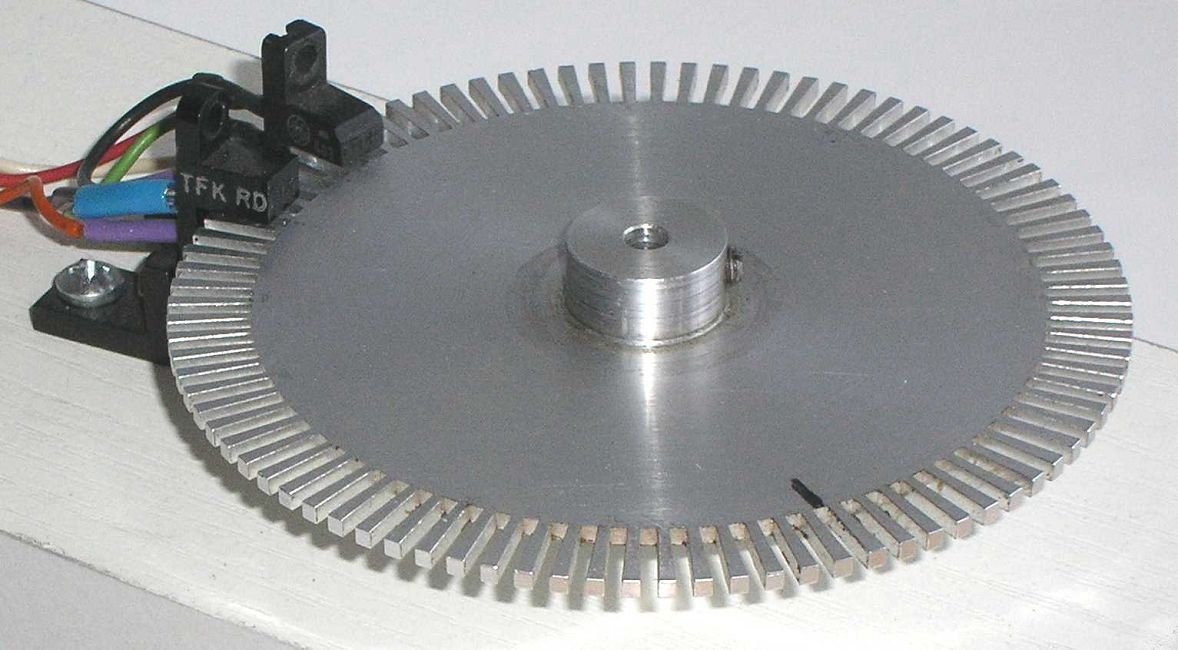
\includegraphics[width=0.7\textwidth]{img/encoder.png}
\caption{Enkoder inkrementalny wykorzystywany w odometrii}
\label{fig:encoder}
\end{figure}

\subsection{Skaner laserowy}
Współcześnie wykorzystywane dalmierze laserowe z funkcją skanowania wykorzystują metodę \textit{time of flight}, polegającą na wysłaniu impulsu świetlnego w danym kierunku i mierzeniu czasu, który upływa do powrotu impulsu odbitego od przeszkody. Na podstawie wartości tego czasu, znając prędkość światła, można wyznaczyć odległość od przeszkody. Aby osiągnąć pełny skan pomieszczenia, taki pomiar jest powtarzany w stałym interwale kątowym, np. $\Delta \phi = 0.50 \degree$ w zakresie 180 $\degree$ lub większym. Zasadę działania skanera zobrazowano na rys. \ref{fig:lidar}. Wynikiem działania skanera jest zbiór par $(r_i, \phi_i)$, określających odległosć od przeszkody i kąt skanowania. Czas wykonania pełnego skanu jest rzędu 10 ms, zaś dokładność pomiaru odległości - rzędu 10 mm.

Skany pomieszczenia w połączeniu z danymi odometrycznymi mogą zostać wykorzystane do zbudowania mapy otoczenia za pomocą algorytmu SLAM (ang. Simultaneouos Localization and Mapping, \textit{Jednoczesna Lokalizacja i Mapowanie}). Mapowanie z użyciem map SLAM polega na dopasowaniu skanu laserowego do konturu mapy i wyliczeniu translacji i rotacji pomiędzy konturem reprezentowanym przez skan laserowy, a konturem mapy, co pozwala na zlokalizowanie robota. Istnieje szereg algorytmów dopasowania skanu do mapy, opisanych szerzej w książce \cite{probabilistic_robotics}. Połączenie danych ze skanera laserowego i odometrii za pomocą filtra cząsteczkowego pozwala na bardzo dobre lokalizowanie robota, zarówno w sytuacji nieznanej mapy (za pomocą SLAM) jak i przy wykorzystaniu już posiadanej mapy.
\begin{figure}[]
\centering
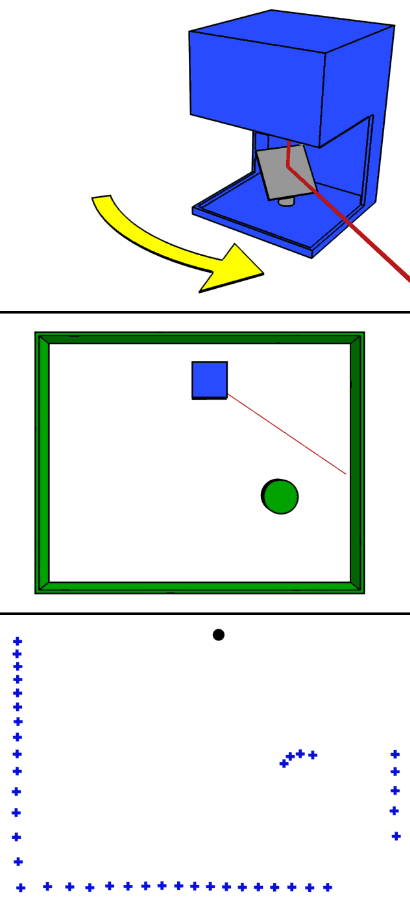
\includegraphics[width=0.5\textwidth]{img/lidar.png}
\caption{Zasada działania skanera laserowego. Od góry: 1. Kierowanie wiązki świetlnej. 2. Skanowane pomieszczenie. 3. Wynikowy zbiór punktów.}
\label{fig:lidar}
\end{figure}

\subsection{Problem porwanego robota}
Problemem porwanego robota nazywamy sytuację, w której robot lokalizowany za pomocą odometrii i/lub skanera losowego zostanie zabrany i przeniesiony do innego otoczenia. Ponieważ takiemu przemieszczeniu robota nie towarzyszy żaden obrót kół, odometria nie jest w stanie go zarejestrować. Natomiast jeśli robot zostanie przeniesiony np. z pomieszczenia o prostokątnym rozkładzie ścian do innego pomieszczenia o identycznym rozkładzie, również skaner laserowy nie będzie w stanie zdeterminować położenia robota. W wypadku lokalizacji za pomocą filtra cząsteczkowego będzie to skutkowało powstaniem dwóch (lub więcej, jeśli jest więcej podobnych pomieszczeń) skupisk cząsteczek, z których nie można jednoznacznie wybrać właściwego położenia. Podobna niejednoznaczność zachodzi często zaraz po uruchomieniu robota, kiedy jego pozycja w globalnym układzie współrzędnych pozostanie nieznana. W takiej sytuacji, dopóki robot nie wykona przejazdu, podczas którego zostaną zarejestrowane punkty charakterystyczne, nie jest możliwe określenie jego lokalizacji. 

Pomocą w takich sytuacjach może okazać się lokalizacja za pomocą znaczników radiowych. Choć jej dokładność jest niższa niż w wypadku skanera laserowego, to zgrubne wskazanie położenia na mapie może rozwiązać niejednoznaczności opisane powyżej i w rezultacie rozwiązać problem porwanego robota. 
\clearpage{\pagestyle{empty}\cleardoublepage}

\chapter{Zastosowanie znaczników radiowych do mierzenia odległości}
\label{ch:radio}
Systemy nawigacji satelitarnej takie jak GPS czy GLONASS, jak i systemy lokalizacji za pomocą sieci komórkowej nie znajdują zastosowania w lokalizacji wewnątrz pomieszczeń. Podstawowymi problemami, na jakie natrafiają te systemy, jest brak zasięgu wewnątrz pomieszczeń i związana z tym zbyt mała dokładność.
Jednocześnie popularyzacja sieci Wi-Fi i standardu komunikacji bezprzewodowej Bluetooth spowodowała, że urządzenia wykorzystujące te standardy są szeroko dostępne i przystępne cenowo. Sieci Wi-Fi i standard Bluetooth operują paśmie ISM (Industrial, Scientific and Medical, częstotliwości rzędu 2.4 GHz). Dobra dostępność tych technologii skłania do wykorzystania ich także w robotyce. 

W niniejszym rozdziale przedstawiono podstawy teoretyczne modelu propagacji fal radiowych w pomieszczeniu, następnie opisano problem modelowania relacji odległość - siła sygnału i możliwe jego rozwiązania. Przedstawiono także najpopularniejsze technologie radiowe pasma ISM, z naciskiem na technologię Bluetooth, wybraną do implementacji rozwiązania. 

\section{Propagacja sygnału radiowego w pomieszczeniu zamkniętym}
Do szacowania poziomu sygnału w modelach propagacyjnych wprowadza się parametr zwany współczynnikiem tłumienności trasy. Opisuje on zmniejszenie poziomu sygnału odbieranego w stosunku do mocy sygnału nadawanego w skutek przejścia fal radiowych przez środowisko propagacyjne wprowadzające pewne tłumienie. Transmisję sygnału radiowego opisuje schemat przedstawiony na rys. \ref{fig:propagacja-fal}. Przez $P_{TX}$ oznaczono moc nadajnika, $G_{TX}$ - zysk anteny nadawczej, $G_{RX}$ - zysk anteny odbiorczej, $L$ - współczynnik tłumienności trasy (ang. \textit{path loss index}), zaś $P_{RX}$ - moc sygnału odebranego \cite{rssi}. 

Współczynnik $L$ opisuje własności propagacyjne środowiska, w którym przekazywany jest sygnał. Obejmuje zatem czynniki takie jak tłumienność trasy, obecność ścian budynków lub innych przeszkód terenowych, obecność innych źródeł promieniowania. Związane z wymienionymi czynnikami zjawiska odbicia, dyfrakcji i interferencji sygnału powodują, że zagadnienie wyznaczenia współczynnika tłumienności jest niezwykle trudne. W związku z tą trudnością, najczęściej stosowane są modele empiryczne, a zatem oparte na pomiarach siły sygnału w danym środowisku. 

Relację mocy sygnału nadanego i mocy odebranej przez odbiornik można wyrazić następująco: 
\begin{equation}
\label{eq:L}
 L = P_{TX} - P_{RX}
\end{equation}

Do obliczenia odległości na podstawie siły sygnału RSSI (ang. \textit{Received Signal Strength Indicator}, wskaźnik siły sygnału sygnału odebranego) należy posłużyć się modelem propagacji:
\begin{equation}
\label{eq:model_propag}
 P_{RX} = P_{TX}+G_{TX}+G_{RX} + 20\log(\lambda) - 20\log(4\pi) -10n\log(d)
\end{equation}

W równaniu \ref{eq:model_propag} przez $d$ oznaczono odległość między transmiterem a odbiornikiem, $\lambda$ oznacza długość fali, zaś współczynnik $n$ określa wpływ przeszkód takich jak ściany. Należy zaznaczyć, że wartości mocy nadajnika $P_{TX}$, zysków anten $G_{RX}$ i $G_{TX}$, długości fali $\lambda$ oraz współczynnika $n$ na ogół nie są znane, podczas gdy moc sygnału odebranego $P_{RX}$ jest zwykle możliwa do określenia, jako że implementacje protokołów radiowych przewidują dołączenie jej wartości do zdekodowanych ramek danych. 

Ponadto, wyznaczenie analityczne współczynnika $n$ jest niemożliwe. Zależy on bowiem bardzo silnie od architektury pomieszczenia, położenia nadajnika względem ścian, podłogi i stropu, a także od zakłóceń. Jako podstawowe źródła zakłóceń sygnału można wyróżnić:

\begin{itemize}
 \item odbiorniki elektryczne dużej mocy, np. kuchenki lub silniki elektryczne,
 \item silne źródła promieniowania, takie jak kuchenki mikrofalowe,
 \item inne nadajniki radiowe korzystające z danego pasma, szczególnie bardzo popularne punkty dostępowe sieci Wi-Fi.
\end{itemize}

Obecność ścian, przedmiotów a także obiektów ruchomych, np. przemieszczających się ludzi, powoduje występowanie odbić i rozproszeń fali radiowej. Pod pewnymi względami może zajść także tzw. efekt falowodowy, wskutek którego fala pokonuje znacznie większą odległość bez tłumienia (dzieje się tak np. w długich korytarzach). Powyższe zjawiska skutkują wzrostem zjawiska wielokrotnego obicia, czyli docierania fali do odbiornika wieloma drogami (np. bezpośrednio z nadajnika i po odbiciu od ściany). To zjawisko jest szczególnie poważną przeszkodą do zastosowania pomiaru siły sygnału RSSI do wyznaczenia odległości. 

\begin{figure}[H]
\centering
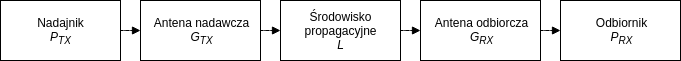
\includegraphics[width=0.7\textwidth]{img/propagacja-fal.png}
\caption{Schemat propagacji fal radiowych}
\label{fig:propagacja-fal}
\end{figure}

\section{Wyznaczanie odległości na podstawie siły sygnału RSSI}
\label{sec:rssi-odleglosc}
Zgodnie z zależnością \ref{eq:model_propag}, wraz ze wzrostem odległości nadajnika i odbiornika, wartość RSSI powinna spadać. Jednakże z powodu zjawisk wymienionych w poprzedniej sekcji, ta zależność nie zawsze jest zachowana. Dla odbiornika pozostającego w stałej odległości od nadajnika, wartość RSSI nie pozostaje stała, co obrazują wyniki eksperymentalne (wykres na rys. \ref{fig:rssi-stacjonarne}). 

\begin{figure}[H]
\centering
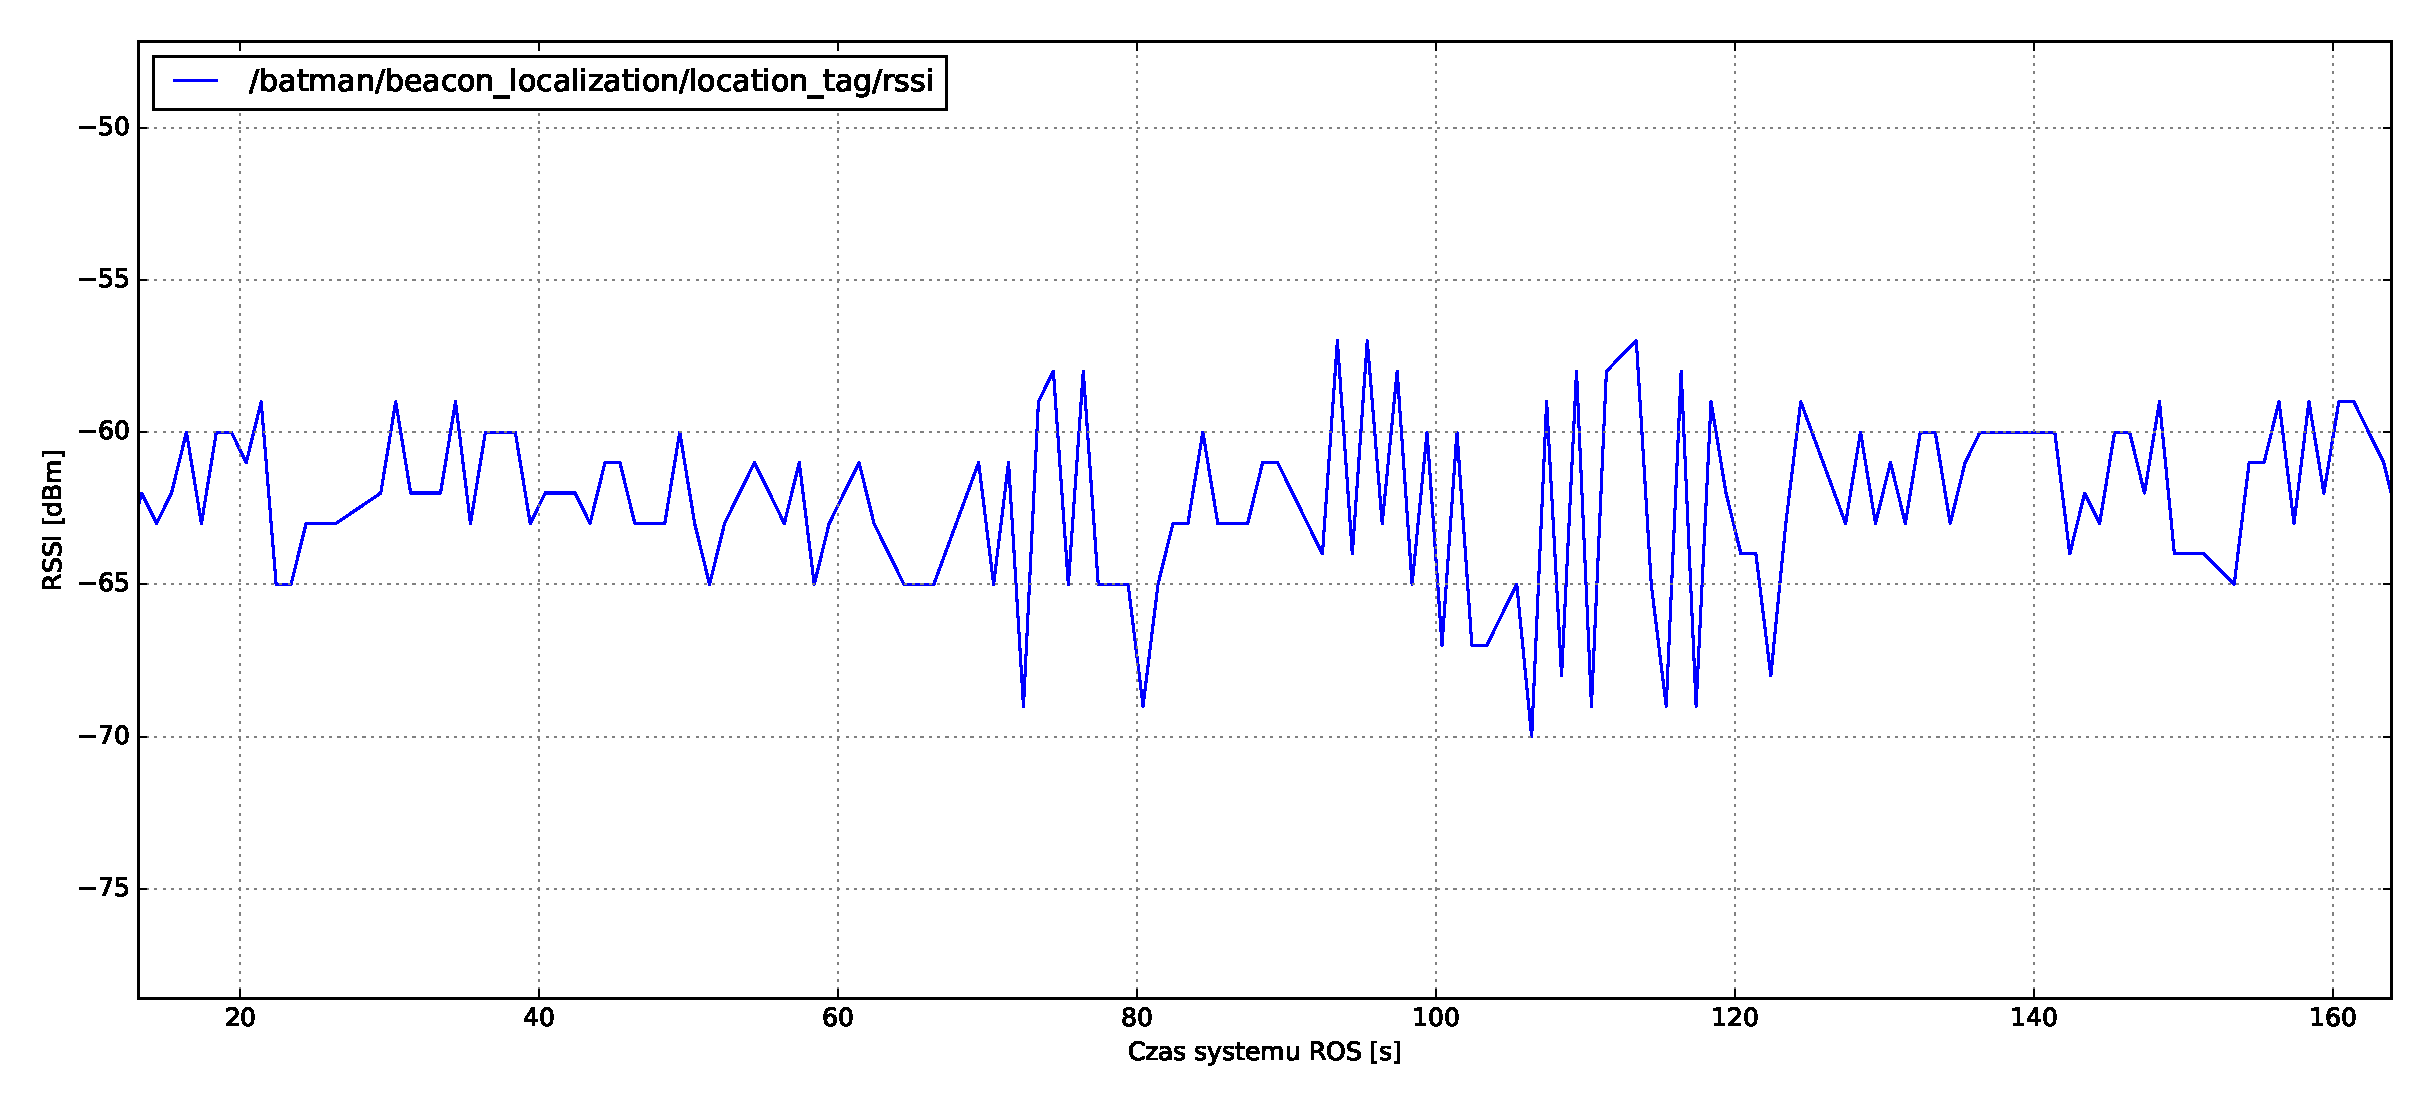
\includegraphics[width=0.85\textwidth]{img/rssi_stacjonarne.eps}
\caption{Przebieg wartości RSSI dla stacjonarnego odbiornika będącego w odległości 70 cm od nadajnika (znacznik BLE). Pominięto pierwsze 15 sekund pomiaru ze względu na stan nieustalony systemu ROS.}
\label{fig:rssi-stacjonarne}
\end{figure}

Jak widać z wykresu \ref{fig:rssi-stacjonarne}, nawet dla nieruchomego odbiornika występują wahania RSSI rzędu 10 dBm. Dlatego konieczne jest zastosowanie filtra wygładzającego. Do wygładzenia wartości RSSI można wykorzystać następujące narzędzia:
\begin{itemize}
 \item filtr oparty o średnią ruchomą prostą lub ważoną,
 \item filtr dolnoprzepustowy,
 \item filtr Kalmana, uwzględniający wiedzę na temat ruchu odbiornika.
\end{itemize}

Projektując filtr RSSI, należy zwrócić szczególną uwagę na bezwładność, jaką wprowadza on do pomiaru, a która utrudnia lub nawet uniemożliwia pomiar odległości dla odbiornika pozostającego w ruchu. W tym kontekście, szczególnie użyteczny jest filtr Kalmana, który może wykorzystać informację o ruchu odbiornika radiowego pochodzącą np. z systemu lokalizacji robota. Szczegóły dotyczące filtracji sygnału RSSI zostały szerzej omówione w rozdziale \ref{ch:metody-lokalizacji}, gdzie opisano proponowany algorytm lokalizacji robota.

Kolejnym problemem związanym z pomiarem odległości za pomocą siły sygnału RSSI jest wyznaczenie zależności siły sygnału RSSI od odległości $P_{RX}(d)$. Wzór \ref{eq:model_propag} zawiera parametry nadajnika i odbiornika oraz medium transmisyjnego, które na ogół nie są znane. Z pomocą przychodzą metody empiryczne. Wykonując serię pomiarów siły sygnału w różnych odległościach od nadajnika i w różnych miejscach pomieszczenia, otrzymuje się zbiór danych który pozwala na wyznaczenie aproksymacji zależności $P_{RX}(d)$. W dalszej części rozdziału opisano podstawowe metody otrzymywania tej aproksymacji.

\subsection{Aproksymacja za pomocą krzywych wielomianowych}
Pierwszym możliwym rozwiązaniem jest dopasowanie krzywej wielomianowej do punktów pomiarowych, proponowane przez autorów artykułu \cite{rssi}. Aproksymowana funkcja ma postać:
\begin{equation}
\label{eq:approx_poly}
  y_{P_{RX}} = a_0 + a_1 d_x + a_2 d_x^2 + ... + a_n d_x^n
\end{equation}

gdzie $a_0, ..., a_n$ są współczynnikami wielomianu stopnia $n$, aproksymującego zależność. Mając $N$ punktów pomiarowych $(d_{xi}, y{P_{RX}i})$, gdzie $i = 1,2, ..., N$, błąd aproksymacji $e_i$ wynosi

\begin{equation}
\label{eq:approx_poly_e}
  e_i = y_{P_{RX}} -( a_0 + a_1 d_x + a_2 d_x^2 + ... + a_n d_x^n )
\end{equation}

Współczynniki $a_0, ..., a_n$ wyznacza się rozwiązując zadanie minimalizacji błędu średniokwadratowego:

\begin{equation}
\label{eq:approx_poly_mse}
  S = \sum_{i=1}^{N} e_i^2
\end{equation}

Wyniki przedstawione w artykule \cite{rssi} wskazują, że najlepsze wyniki dają aproksymacje wielomianami niskiego rzędu $n=2, n=3$

\subsection{Interpolacja}
Kolejną metodą aproksymowania zależności $P_{RX}(d)$ proponowaną przez \cite{rssi} jest interpolacja. Pozwala ona na wyeliminowanie niewiadomych składników równania. Rozważmy dwa wybrane pomiary. Oznaczając je indeksami 1 i 2 oraz podstawiając do równania \ref{eq:model_propag} otrzymujemy:

\begin{equation}
\label{eq:interpol_podst1}
 P_{RX1} = P_{TX}+G_{TX}+G_{RX} + 20\log(\lambda) - 20\log(4\pi) -10n\log(d_1)
\end{equation}
\begin{equation}
\label{eq:interpol_podst2}
 P_{RX2} = P_{TX}+G_{TX}+G_{RX} + 20\log(\lambda) - 20\log(4\pi) -10n\log(d_2),
\end{equation}
gdzie $P_{RX}$ jest mocą odebranego sygnału, $P_{TX}$ - mocą sygnału nadawanego, $G_{RX}$ i $G_{TX}$ odpowiednio wzmocnieniem anteny odbiorczej i nadawczej, $\lambda$ - długością fali sygnału radiowego, zaś $d$ - odległością odbiornika od nadajnika. 

Odjęcie powyższych równań stronami pozwala wyeliminować niewiadome zależne od sprzętowych aspektów nadajnika i odbiornika, a następnie wyprowadzić zależność interpolowaną postaci:
\begin{equation}
\label{eq:interpol}
 P_{RX} = (P_{RX1}-P_{RX2}) \frac{\log{d} - \log{d_2}}{\log{d_1} - \log{d_2}} + P_{RX2}
\end{equation}

Wykorzystując dwa punkty pomiarowe i zależność \ref{eq:interpol} można otrzymać aproksymację zależności RSSI od odległości. Punkty do interpolacji należy dobrać eksperymentalnie, aby osiągnąć optymalne wyniki. 

\subsection{Dopasowanie krzywej logarytmicznej lub wykładniczej}
Łatwo zauważyć, że w równaniu \ref{eq:model_propag} część składników jest stała i zależy od uwarunkowań sprzętowych nadajnika i odbiornika, bądź warunków środowiskowych. Grupując składniki stałe można napisać:

\begin{equation}
\label{eq:logfit}
 P_{RX} = A + B \log(d)
\end{equation}

gdzie:

\begin{equation}
\label{eq:logfitA}
A = P_{TX}+G_{TX}+G_{RX} + 20\log(\lambda) - 20\log(4\pi)
\end{equation}

\begin{equation}
\label{eq:logfitB}
B = -10n
\end{equation}

Wykorzystując narzędzia optymalizacyjne, dostarczane przez pakiety takie jak MATLAB lub bibliotekę SciPy można wykonać dopasowanie krzywej logarytmicznej do punktów pomiarowych, aby otrzymać zależność postaci \ref{eq:logfit} \cite{scipy}. Dokonując odpowiednich przekształceń, można łatwo wyznaczyć także zależność odwrotną, faktycznie potrzebną w zadaniu lokalizacji. Ma ona postać:

\begin{equation}
\label{eq:logfit_d}
d = 10 ^ {\frac{P_{RX}-A}{B}}
\end{equation}

W dalszej części rozdziału opisano popularne technologie radiowe, możliwe do wykorzystania w lokalizacji robota mobilnego. 

\section{Protokół Wi-Fi}
\label{sec:wifi}
Nazwa Wi-Fi (ang. Wireless Fidelity, \textit{Bezprzewodowa wierność}) jest potocznym określeniem zestawu standardów określających budowę bezprzewodowych sieci komputerowych, w szczególności sieci WLAN, czyli bezprzewodowych sieci lokalnych. Wi-Fi wykorzystuje częstotliwości pasma ISM: 2.4 GHz oraz 5.8 GHz. Warstwa fizyczna oraz podwarstwa MAC jest opisywana przez grupę standardów IEEE 802.11. Duża popularność sieci Wi-Fi w budynkach sprawia, że rozwiązanie to dobrze nadaje się do zastosowania w lokalizacji. Istnieje szereg opracowań naukowych wykorzystujących technologię Wi-Fi do lokalizacji wewnątrz pomieszczeń (\cite{fingerprinting}), nie tylko w robotyce, ale także m. in. do lokalizowania osób posiadających telefon komórkowy (\cite{rssi}). Zasilanie sieciowe punktów dostępych pozwala na szybkość transmisji danych znacznie większą niż w innych technologiach radiowych. Jednakże, wadą rozwiązania jest duże zużycie energii, szczególnie po stronie odbiornika który często zasilany jest bateryjnie, oraz koszt urządzeń i ich instalacji większy niż w wypadku opisanego dalej Bluetooth. 


\section{Protokół Bluetooth}
\label{sec:bluetooth}
Bluetooth jest standardem komunikacji bezprzewodowej, zaprojektowanym do wymiany danych na krótkie dystanse, korzystający z fal krótkich UHF pasma ISM (częstotliwości rzędu 2.4 GHz). Standard Bluetooth jest zarządzany przez organizację Bluetooth Special Interest Group (SIG), będącą zrzeszeniem firm z branż komunikacyjnej, sieciowej, informatycznej i elektronicznej \cite{ble}. 

Pasmo ISM (ang. \emph{Industrial, Scientific and Medical}, Przemysłowe, Naukowe i Medyczne) wykorzystywane przez Bluetooth jest nielicencjonowane. Dla zapewnienia odporności na zakłócenia, Bluetooth wykorzystuje technologię rozpraszania widma FHSS (ang. \emph{Frequency Hopping Spread Spectrum}) polegającą na "skakaniu" po częstotliwościach dostępnych w paśmie w kolejnych odstępach czasu. Protokół Bluetooth jest oparty o pakiety, ze strukturą master-slave \cite{ble}. 

\subsection{Bluetooth Low Energy}
\label{sec:ble}
Bluetooth Low Energy, znane także pod nazwą handlową Bluetooth Smart, jest czwartą wersją specyfikacji standardu Bluetooth. Standard ten został zorientowany na zapewnienie transmisji o minimalnym koszcie energetycznym. Podstawowe cechy BLE to: 
\begin{itemize}
 \item niskie zużycie energii, pozwalające urządzeniom operować przez długi (rzędu roku) czas na jednej baterii guzikowej,
 \item mały rozmiar i koszt urządzeń,
 \item kompatybilność z popularnymi urządzeniami obecnymi na rynku (smartfony, tablety, laptopy).
\end{itemize}

Dla osiągnięcia efektywności energetycznej BLE wykorzystuje odmienny w stosunku do klasycznego Bluetooth model komunikacji. Występują dwa tryby pracy:
\begin{itemize}
 \item tryb rozgłoszeniowy (ang. \emph{advertising mode}),
 \item tryb połączenia (ang. \emph{connection mode}).
\end{itemize}

W trybie rozgłoszeniowym urządzenie wysyła pakiety nieskierowane do żadnego odbiornika w stałym interwale czasowym. Pomiędzy nadawaniem procesor oraz radio urządzenia mogą pozostawać w stanie uśpienia, co pozwala na znaczną oszczędność energii. Pojedynczy pakiet rozgłoszeniowy zawiera 31 bajtów użytecznych danych i może być odebrany przez dowolne urządzenie w trybie nasłuchu (ang. \emph{scan mode}). 
Nasłuchujące odbiorniki, po przechwyceniu pakietu rozgłoszeniowego i tym samym odkryciu urządzenia nadawczego, mogą nawiązać z nim połączenie. Tryb połączenia, podobnie jak w klasycznym Bluetooth, jest nawiązywany pomiędzy dwoma urządzeniami i służy do wymiany danych pomiędzy nimi. Przebywając w trybie rozgłoszeniowym, średnie zużycie prądu przez urządzenie Bluetooth może pozostawać na poziomie $\mathbf{\mu}$A, co pozwala osiągnąć wspomniane wcześniej długie czasy pracy na baterii. Ma to szczególne znaczenie w robotyce mobilnej, gdzie roboty na ogół pracują na zasilaniu akumulatorowym. 





\clearpage{\pagestyle{empty}\cleardoublepage}

\chapter{Metody lokalizacji na podstawie znaczników radiowych}
\label{ch:metody-lokalizacji}

Znaczniki radiowe, rozmieszczone w ustalonych miejscach środowiska pracy robota, pozwalają na podjęcie zadania lokalizacji na kilka różnych sposobów. W niniejszym rozdziale przedstawiono podstawowe metody lokalizacji.

\section{Fingerprinting}
Metoda fingerprintingu (ang.\textit{fingerprint} - odcisk palca) opiera się na zbiorze punktów referencyjnych. Punkty referencyjne zbiera się w fazie off-line, zapisując w bazie danych położenie danego punktu w przestrzeni oraz referencyjny wektor RSSI postaci $P_{ref} = [ P_{ref \ 1} \cdots P_{ref  \ N}]$, gdzie $N$ jest liczbą znaczników w środowisku, zaś $P_{ref \ i}$ oznacza siłę sygnału RSSI z $i$-tego znacznika \cite{fingerprinting}. Przykładowe rozmieszczenie znaczników i punktów referencyjnych pokazuje schemat na rys. \ref{fig:fingerprinting}.


\begin{figure}[H]
\centering
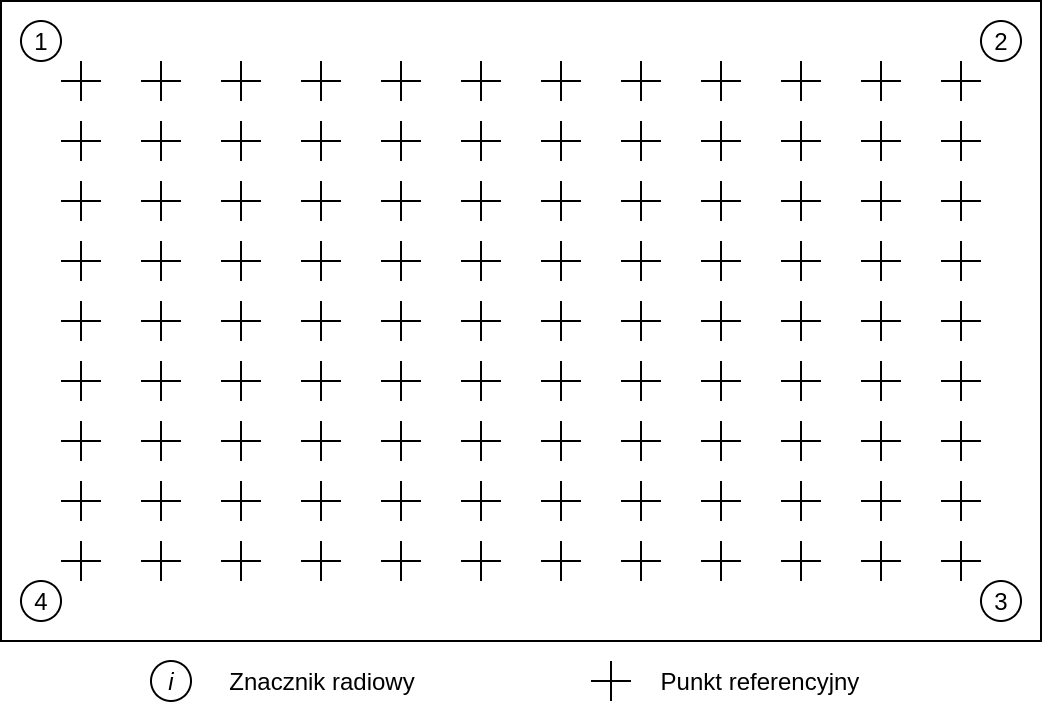
\includegraphics[width=0.7\textwidth]{img/fingerprinting.png}
\caption{Rozmieszczenie znaczników radiowych i punktów referencyjnych w metodzie fingerprintingu. Znaczniki radiowe oznaczono kółkami z cyfrą, punkty referencyjne }
\label{fig:fingerprinting}
\end{figure}

W fazie on-line lokalizowany odbiornik rejestruje wektor siły sygnału $P = [ P_{RX \ 1} \cdots P_{RX \ n}]$ dla danego położenia, następnie obliczana jest odległość wektora $P$ od wektorów referencyjnych $P_{ref}$ według metryki euklidesowej \cite{fingerprinting2}:


\begin{equation}
\label{eq:fingerprinting_odleglosc}
 D(Z, Z_i) = \sqrt{\sum_{j=1}^{N} (P_{ref \ i \ j}-P_{RX \ j})^2}.
\end{equation}

Z odległością \ref{eq:fingerprinting_odleglosc} jako kryterium, można wyszukać K najbliższych sąsiadów wektora $P_{RX}$ w zbiorze punktów referencyjnych $P_{ref}$. Publikacja \cite{fingerprinting2} proponuje następujące podejścia:
\begin{enumerate}
 \item $K = 1$ - za wynik lokalizacji przyjmowany jest najbliższy punkt referencyjny,
 \item $K > 1$ - za wynik lokalizacji przyjmowany jest środek ciężkości najbliższych $K$ punktów referencyjnych.
\end{enumerate}

Wyszukiwanie sąsiadów można prowadzić na pełnym zbiorze punktów referencyjnych lub tylko na jego części, ograniczonej np. do pewnego promienia wokół poprzedniej pozycji. Pozwala to na przyspieszenie wyszukiwania \cite{fingerprinting}. Jakość lokalizacji można dodatkowo poprawić wykorzystując metody probabilistyczne takie jak filtr Bayesa lub cząsteczkowy \cite{fingerprinting2}.

Niewątpliwą zaletą lokalizacji w oparciu o fingerprinting jest to, iż uwzględnia ona nieizotropowy rozkład siły sygnału RSSI w zależności od położenia odbiornika. Ponadto nie jest konieczne wyznaczanie modelu propagacji radiowej do przeliczania RSSI na odległość. Jeśli siatka punktów referencyjnych jest odpowiednio gęsta, fingerprinting jest w stanie zapewnić zadowalające rezultaty. Z drugiej strony, lokalizacja tą metodą wymaga przeprowadzenia dość złożonej kalibracji w fazie off-line (budowanie zbioru punktów referencyjnych), ponadto konieczne jest zapewnienie metody wydajnego przeszukiwania zbioru referencyjnego, zaś jeśli zbiór ten zawiera mało punktów, jakość lokalizacji może być niezadowalająca. 


\section{Trilateracja}
\label{sec:trilateracja}
Trilateracja, obok triangulacji, jest jedną z metod geometrycznych wyznaczania położenia obiektu za pomocą pomiaru kąta lub odległości względem ustalonego węzła. Triangulacja opiera się na pomiarze kątów, natomiast trilateracja - odległości. Dzięki temu możliwe jest zastosowanie jej w lokalizacji w oparciu o pomiar siły sygnału RSSI, związanej z odległością. 

Zadanie trilateracji polega na wyznaczeniu położenia lokalizowanego obiektu, znając odległości tego obiektu od 3 (przypadek dwuwymiarowy) lub 4 (przypadek trójwymiarowy) punktów referencyjnych o znanym położeniu. W dalszej części pracy rozważany będzie tylko przypadek dwuwymiarowy. Oznaczmy $i$-ty punkt referencyjny przez $O_i(x_i, y_i)$. Odległość punktu referencyjnego od lokalizowanego obiektu znajdującego się w punkcie $P(x,y)$ wynosi $R_i$ (rys. \ref{fig:trilateracja-ideal}). O ile punkty $O_i$ nie są współliniowe, punkt $P$ znajduje się na przecięciu okręgów $(O_1, R_1)$, $(O_2, R_2)$, $(O_3, R_3)$. Dlatego rozwiązanie zadania trilateracji można zapisać następująco \cite{trilat_przeglad}:

\begin{equation}
\label{eq:trilateracja1}
 (x - x_1)^2 + (y-y_1)^2 = R_1^2
\end{equation}
\begin{equation}
 (x - x_2)^2 + (y-y_2)^2 = R_2^2
\end{equation}
\begin{equation}
\label{eq:trilateracja3}
 (x - x_3)^2 + (y-y_3)^2 = R_3^2
\end{equation}

Jest to układ równań nieliniowych. Ponieważ liczba punktów referencyjnych może być większa od 3, możemy mieć do czynienia z układem nadokreślonym. Do rozwiązania takiego układu można wykorzystać metodę macierzy pseudo-odwrotnych \cite{trilat_particle}. Generalnie, analityczne rozwiązanie takiego układu równań przedstawia znaczne trudności lub jest niemożliwe \cite{trilat_przeglad}, natomiast rozwązanie numeryczne jest obarczone znacznym błędem \cite{trilat_particle}. Ponadto, w realistycznym przypadku, okręgi nie będą przecinać się w jednym punkcie. Możliwe jest, że będzie więcej punktów przecięcia (rys. \ref{fig:trilateracja-real1}) lub okręgi nie będą się przecinać (rys. \ref{fig:trilateracja-real2}). W obu tych przypadkach powyższy układ równań nie będzie miał rozwiązań. 


\begin{figure}[h]
\centering
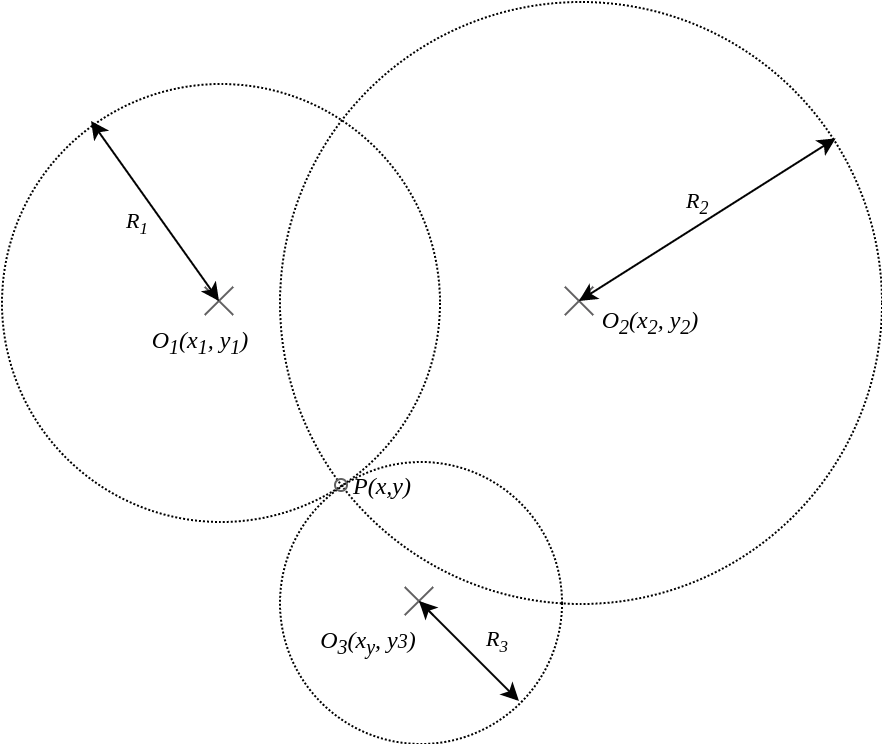
\includegraphics[width=0.6\textwidth]{img/trilateracja-okregi1.png}
\caption{Trilateracja - przypadek idealny}
\label{fig:trilateracja-ideal}
\end{figure}

\begin{figure}[h]
\centering
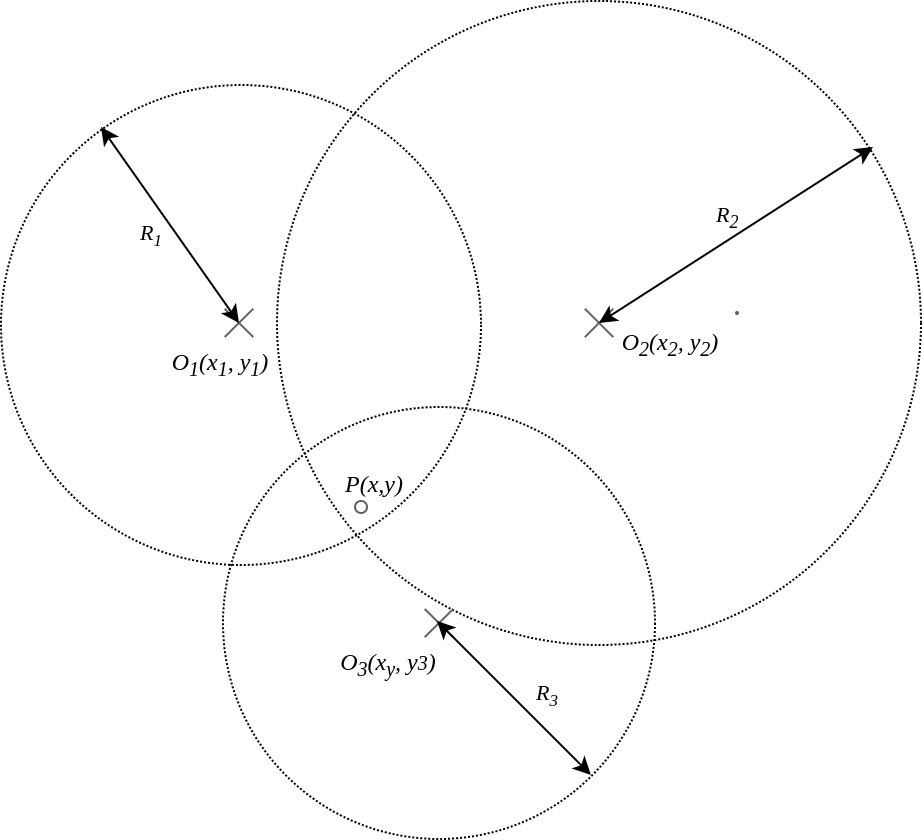
\includegraphics[width=0.6\textwidth]{img/trilateracja-okregi2.png}
\caption{Trilateracja - przypadek rzeczywisty - okręgi nakładają się}
\label{fig:trilateracja-real1}
\end{figure}

\begin{figure}[h]
\centering
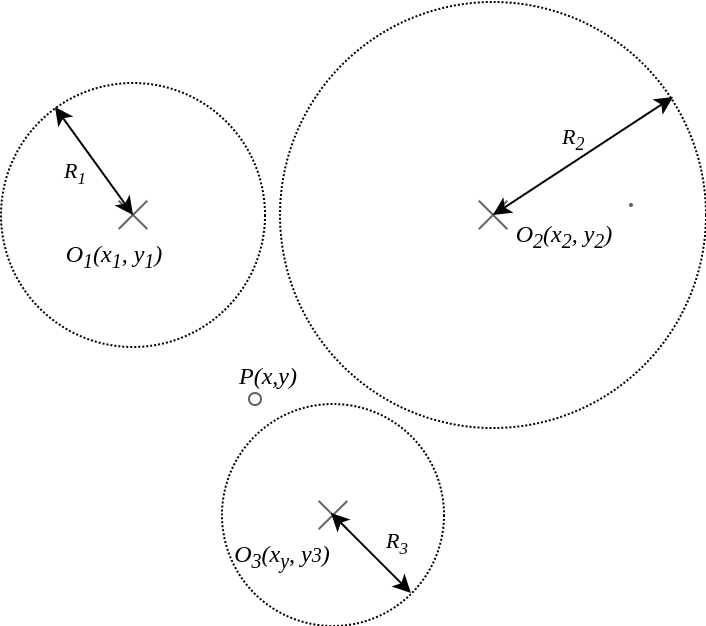
\includegraphics[width=0.6\textwidth]{img/trilateracja-okregi3.png}
\caption{Trilateracja - przypadek rzeczywisty - okręgi wogóle się nie przecinają}
\label{fig:trilateracja-real2}
\end{figure}


W celu osiągnięcia dobrego rozwiązania numerycznego zadania trilateracji, można posłużyć się algorytmem iteracyjnym \cite{trilat_iter}. Algorytm wymaga, żeby znane były położenia co najmniej 3 punktów referencyjnych $(x_i, y_i)$, oraz zmierzone odległości lokalizowanego obiektu od tych punktów $R_i$, oraz początkowa estymata rozwiązania $(x_e, y_e)$. W każdej iteracji obliczana jest różnica między zmierzoną, a estymowaną odległością obiektu od każdego punktu referencyjnego:

\begin{equation}
\label{eq:trilateracja_iter_f}
f_i = | d_i - \sqrt{(x_i - x_e)^2 + (y_i-y_e)^2}|
\end{equation}


Oznaczając przez $\vec R_ {k}$ estymatę rozwiązania w $k$-tej iteracji:
\begin{equation}
\vec R_ {k} = \left( \begin{array}{c} 
x_{e} \\
y_{e} \\
\end{array} \right)
\end{equation}

i posługując się metodą Newtona \cite{trilat_przeglad} możemy przedstawić równanie następnej iteracji:

\begin{equation}
\label{eq:trilateracja_iter}
\vec R_ {k+1} = \vec R_ {k} - (\mathbf{J}_{k}^T \mathbf{J}_{k})^{-1} \mathbf{J}_{k}^T \vec f_{k}
\end{equation}

gdzie:

\begin{equation}
\label{eq:f_wektor}
\vec f_{k} = \left( \begin{array}{c} 
f_{1} \\
f_{2} \\
\vdots \\
f_{n} \\
\end{array} \right) ,
\end{equation}

zaś przez $\mathbf{J}_{k}$ oznaczamy macierz Jakobiego funkcji $f$:

\begin{equation}
\label{eq:J_wektor}
\mathbf{J}_{k} = 
\left( \begin{array}{cc} 
  \frac{\partial f_{1} }{\partial x} & \frac{\partial f_{1} }{\partial y} \\
  \frac{\partial f_{2} }{\partial x} & \frac{\partial f_{2} }{\partial y} \\
  \vdots & \vdots \\	
  \frac{\partial f_{n} }{\partial x} & \frac{\partial f_{n} }{\partial y} \\
\end{array} \right) = 
\left( \begin{array}{cc} 
  \frac{(x_1 - x_e) }{\sqrt{(x_i - x_e)^2 + (y_i-y_e)^2}} & \frac{(y_1 - y_e) }{\sqrt{(x_i - x_e)^2 + (y_i-y_e)^2}} \\
  \frac{(x_2 - x_e) }{\sqrt{(x_i - x_e)^2 + (y_i-y_e)^2}} & \frac{(y_2 - y_e)  }{\sqrt{(x_i - x_e)^2 + (y_i-y_e)^2}} \\
  \vdots & \vdots \\	
  \frac{(x_3 - x_e)}{\sqrt{(x_i - x_e)^2 + (y_i-y_e)^2}} & \frac{(y_n - y_e)  }{\sqrt{(x_i - x_e)^2 + (y_i-y_e)^2}} \\
\end{array} \right).
\end{equation}

Aby wyznaczyć rozwiązanie zadania trilateracji, należy wykonywać kolejne iteracje metody Newtona zgodnie z równaniem \ref{eq:trilateracja_iter}. Jako estymatę początkową można przyjąć np. rozwiązanie zlinearyzowanego układu równań \ref{eq:trilateracja1} - \ref{eq:trilateracja3}.

W porównaniu do fingerprintingu, trilateracja nie wymaga złożonej fazy off-line. Z drugiej strony, jeśli do pomiaru odległości wykorzystywana jest siła sygnału RSSI, pomiar jest obarczony wszystkimi błędami opisanymi w rozdziale \ref{ch:radio}, w szczególności nie ma możliwości, aby uwzględnić nieizotropowy rozkład siły sygnału w pomieszczeniu. 

\section{Filtr cząsteczkowy}
\label{sec:filtr-czasteczkowy}
Filtr cząsteczkowy, należący do metod Monte Carlo, jest bardzo popularnym narzędziem w robotyce mobilnej. Jest to nieparametryczny, quasi-bayesowski filtr probabilistyczny, pozwalający na reprezentowanie stanu robota w postaci funkcji gęstości prawdopodobieństwa, radzący sobie z nie-gaussowskimi i nieliniowymi modelami pomiaru. Poniżej przedstawiono podstawy teorii filtrów cząsteczkowych oraz możliwe zastosowanie w lokalizacji na podstawie odległości od znaczników radiowych. 

W filtrze cząsteczkowym stan robota jest traktowany jako zmienna losowa $x \in X$. Dla robota poruszającego się na płaszczyźnie lokalizacja opisywana jest przez trzy współrzędne:  $ x = (x, y, \theta)$, gdzie $x$, $y$ są współrzędnymi pojazdu w układze współrzędnych związanym z środowiskiem pracy, zaś $\theta$ jest orientacją robota w tym układzie. Rozkład gęstości prawdopodobieństwa położenia robota $p(x_k | z_k)$ w chwili $k$  jest reprezentowany przez dyskretny zbiór $N_p$ cząsteczek, z których każda reprezentuje hipotezę na temat położenia robota $x_i$ oraz przypisaną jej wagę $w_i$, opisującą stopień potwierdzenia tej hipotezy \cite{preskrypt}, \cite{probabilistic_robotics}:

\begin{equation}
 \label{eq:pf_sk}
 S_{k} = \{ x_i, w_i \}, i = 0, 1, \cdots, N_p, 0 \leq w_i \leq 1,
\end{equation}

Algorytm filtra cząsteczkowego składa się z kilku etapów: 
\begin{enumerate}
 \item \textit{Faza predykcji.} Obliczany jest rozkład gęstości a posteriori w chwili $k$:  $p(x_{k} | x_{k-1}, u_{k-1})$ na podstawie rozkładu gęstości prawdopodobieństwa położenia robota w chwili poprzedniej $p(x_{k-1} | z_{k-1})$ oraz wektora sterowań $u_{k-1}$. Uwzględniany jest model ruchu robota -najczęściej wykorzystywane są sensory odometryczne. Akcja sterowania $u_{k-1} $ jest aplikowana dla każdej cząsteczki ze zbioru $S_{k-1}$. W wyniku powyższej operacji otrzymujemy uaktualniony zbiór cząsteczek:
 \begin{equation}
 \label{eq:pf_sk2}
 S'_{k} = \{ x'_i, w'_i \}, i = 0, 1, \cdots, N_p.
\end{equation}

\item \textit{Pomiar.} Na podstawie pomiaru każdej cząsteczce ze zbioru $S'_{k}$ przypisywana jest nowa waga $w_i$. Wagi są wyznaczane na podstawie rozkładu gęstości prawdopodobieństwa pomiaru: $p(z_{k} | x_{k} )$. Wynikiem jest nowy zbiór $S_{k}$, którego wagi są normalizowane:
\begin{equation}
 w_i = \frac{w_i}{\sum_{j=1}^{N_p} w_j}
\end{equation}

Wagi cząsteczek w nowym zbiorze $S_{k}$ estymują rozkład gęstości prawdopodobieństwa położenia robota $p(x_{k} | z_{k})$.

\item \textit{Resampling}. Po kilku iteracjach wg. punktów 1 i 2, większość cząsteczek miała by pomijalnie małe wagi, przez co estymacja gęstości prawdopodobieństwa $p(x_{k} | z_{k})$ byłaby mało dokładna (estymowana małą ilością cząsteczek). Stąd konieczność dokonania resamplingu cząsteczek (ang. ponowne próbkowanie). Cząsteczki o największych wartościach wag $w_i$ są powielane w zbiorze, natomiast cząsteczki o małych wagach są usuwane ze zbioru \cite{preskrypt}. Resampling jest zagadnieniem złożonym i istnieje kilka różnych algorytmów do wykonania tego zadania \cite{trilat_particle}, \cite{particle_pl}.

\item \textit{Wyznaczenie położenia robota.} Na podstawie zbioru cząsteczek $S_{k}$ należy wyznaczyć położenie robota, będące wynikiem działania filtra. Jako położenie robota można przyjąć położenie reprezentowane przez cząsteczkę o największej wadze, lub średnią ważoną cząsteczek (lub średnią ważoną cząsteczek w pewnym otoczeniu cząsteczki o największej wadze) \cite{preskrypt}:

\begin{equation}
 x_{k} = \sum_{j=0}^{N_p} w_j \cdot x_j
\end{equation}

\end{enumerate}

\subsection{Filtr cząsteczkowy dla robota wyposażonego w sensor odometryczny i system pomiaru odległości od znaczników}
Rozważmy robota o napędzie różnicowym, wyposażonego w sensory odometryczne oraz system wyznaczania odległości od znaczników znajdujących się w ustalonych miejscach środowiska pracy robota, np. system działający w oparciu o znaczniki radiowe. Stan robota jest opisywany przez wektor $x$ postaci:

\begin{equation}
\label{eq:x_wektor}
x_{k} = \left( \begin{array}{c} 
x \\
y \\
\theta \\
\end{array} \right) 
\end{equation}.

\subsubsection{Model ruchu}

Ruch robota, rozumiany jako względna różnica dwóch położeń $x_{k-1} = (x \ y \ \theta)^T$ oraz $x_k = (x' \ y' \ \theta')^T$, może być zamodelowany jako złożenie trzech ruchów prostych: obrotu o kąt  $\delta_{rot1}$, przemieszczenia prostoliniowego o długość $\delta_{trans}$ oraz obrotu o kąt $\delta_{rot2}$. Mając dane dwa wektory położenia robota, $x_{k-1}$ oraz $x_k$, parametry tych ruchów prostych można wyznaczyć następująco \cite{probabilistic_robotics}:
\begin{equation}
 \delta_{rot1} = \mathrm{atan2} (y' - y, x'-x) - \theta,
\end{equation}
\begin{equation}
 \delta_{trans} = \sqrt{(x-x')^2+(y-y')^2},
\end{equation}
\begin{equation}
 \delta_{rot2} = \theta' - \theta - \delta_{rot1}.
\end{equation}
Aby uwzględnić błąd wyznaczenia przemieszczenia, należy uwzględnić szum pomiarowy $\varepsilon_b$ o rozkładzie normalnym, zerowej wartości średniej i wariancji $b$:
\begin{equation}
 \hat \delta_{rot1} = \delta_{rot1} - \varepsilon_{\alpha_1 |\delta_{rot1}|+\alpha_2 |\delta_{trans}|},
\end{equation}
\begin{equation}
 \hat \delta_{trans} = \delta_{trans} - \varepsilon_{\alpha_3 |\delta_{trans}|+\alpha_4 |\delta_{rot1} + \delta_{rot2}|},
\end{equation}
\begin{equation}
 \hat \delta_{rot2} = \delta_{rot2} - \varepsilon_{\alpha_1 |\delta_{rot2}|+\alpha_2 |\delta_{trans}|}.
\end{equation}
Parametry $\alpha_1, \cdots, \alpha_4$ są zależne od budowy robota.

Ostatecznie, równanie uaktualnienia ze stanu $x_{k-1}$ do stanu $x_{k}$ wygląda następująco \cite{probabilistic_robotics}:
\begin{equation}
\label{eq:particle_update}
x_{k} = \left( \begin{array}{c} 
x' \\
y' \\
\theta' \\
\end{array} \right) = \left( \begin{array}{c} 
x \\
y \\
\theta \\
\end{array} \right) + \left( \begin{array}{c} 
\hat \delta_{trans} \cos (\theta + \hat \delta_{rot1}) \\
\hat \delta_{trans} \sin (\theta + \hat \delta_{rot1}) \\
\theta + \hat \delta_{rot1} \hat \delta_{rot2} \\
\end{array} \right)
\end{equation}
To równanie jest używane do predykcji stanu robota w kroku 1 algorytmu filtra cząsteczowego. 

\subsubsection{Model pomiaru}
Zadaniem modelu pomiaru w lokalizacji Monte Carlo jest estymowanie rozkładu gęstości prawdopodobieństwa położenia robota na podstawie mapy otoczenia i pomiarów. Zakładamy, że w otoczeniu robota znajdują się znaczniki (ang. \textit{landmarks}) które można jednoznacznie rozróżnić, zaś ich położenie na mapie jest dokładnie znane. Znacznik taki jest opisywany przez trójkę $(x, y, b)$, gdzie $x, y$ to położenie znacznika w środowisku pracy robota, zaś $b$ jest unikalną wartością dyskretną, identyfikującą znacznik. Mapa środowiska robota jest wtedy wektorem \cite{landmarks}:
\begin{equation}
 M = (m_1,  ..., m_n) = \left( 
  \left( \begin{array}{c} 
x_1 \\
y_1 \\
b_1 \\
\end{array} \right),
\cdots,
  \left( \begin{array}{c} 
x_n \\
y_n \\
b_n \\
\end{array} \right)
\right)
\end{equation}
Obserwowany znacznik jest nazywany cechą (ang. \textit{feature}) i jest reprezentowany przez parę $(r, b)$, gdzie $r$ jest zmierzoną odległością od znacznika, zaś $b$ jego identyfikatorem. W danej chwili czasu $k$ pomiar opisywany przez wektor obserwowanych cech \cite{landmarks}:
\begin{equation}
 f(z) = (f_1,  ..., f_n) = \left( 
  \left( \begin{array}{c} 
r_1 \\
b_1 \\
\end{array} \right),
  \left( \begin{array}{c} 
r_2 \\
b_2 \\
\end{array} \right),
\cdots
\right)
\end{equation}
Każda z cech odnosi się do konkretnego znacznika. Wprowadźmy funkcję dopasowującą, która na podstawie cechy i mapy przypisuje cechę do znacznika: $c(f_i, M)$. W rozpatrywanym przypadku, funkcja dopasowująca odnajduje znacznik na podstawie jego identyfikatora $b$. Następnie wyznaczmy odległość (euklidesową) pomiędzy hipoteczną pozycją robota $\hat p$ a zaobserwowanym znacznikiem $m$:
\begin{equation}
 \label{eq:hatri}
 \hat r_i = \sqrt{(m_x - \hat p_x)^2 + (m_y - \hat p_y)^2}
\end{equation}
oraz różnicę międy zmierzoną odległością od znacznika, a odległością wynikłą z hipotetycznej pozycji $\hat p$ (równanie \ref{eq:hatri}):
\begin{equation}
\Delta r_i = r_i - \hat r_i 
\end{equation}
Do zastosowania w filtrze cząsteczowym potrzebny jest rozkład prawdopodobieństwa wystąpienia wektora pomiarów $f(z)$ dla danej hipotetycznej pozycji $\hat p$ i mapy $M$. Wynika on ze złożenia rozkładów prawdopodobieństwa zaobserwowania poszczególnych cech. Ponieważ zaobserwowanie poszczególnych cech to zdarzenia niezależne, można napisać:
\begin{equation}
 p(f(z) | \hat p, M) = \prod_i p(f_i | \hat p, M)
\end{equation}
Rozkład prawdopodobieństwa danej cechy jest złożeniem prawdopodobieństw zaobserwowania znacznika w danej odległości i o danym identyfikatorze. Po raz kolejny słuszne jest założenie niezależności tych obserwacji. Ponadto, można założyć że system pomiarowy wyznacza identyfikator znacznika w sposób pewny: $p(b | \hat p, M) = 1$. To prowadzi do ostatecznego równania na wiarygodność pomiaru:
\begin{equation}
p(f_i | \hat p, M) = p(r_i | \hat p, M)
\end{equation}
Wiarygodność pomiaru odległości można zamodelować np. rozkładem normalnym o odchyleniu standardowym $\sigma$ :
\begin{equation}
 p(r_i | \hat p, M) = \frac{1}{\sigma \sqrt{2\pi}} \mathrm{exp} \left( \frac{- \Delta r_i}{2\sigma^2} \right)
\end{equation}
Tak wyznacznoną wiarygodność można wykorzystać w kroku 2 filtra cząsteczkowego do uaktualnienia wag cząsteczek zgodnie z wynikiem pomiaru. 




\clearpage{\pagestyle{empty}\cleardoublepage}

\chapter{Projekt systemu lokalizacji robota}
\label{ch:system}

W niniejszym rozdziale przedstawiono projekt systemu lokalizacji robota, opartego na znacznikach radiowych. Jego zadaniem jest akwizycja i filtrowanie danych ze znaczników radiowych, konwersja wartości siły sygnału RSSI na odległość, oraz rozwiązywanie zadania lokalizacji na podstawie zebranych danych. 

System akwizycji danych został zaprojektowany w taki sposób, aby możliwe było eksperymentalne porównanie różnych metod lokalizacji. 

\section{Platforma sprzętowa}
\label{sec:hardware}
\subsection{Znacznik radiowy}
\label{subsec:znacznik}

\subsubsection{Protokół}
Znacznik radiowy do wykorzystania w systemie lokalizacji robota winien spełniać szereg wymagań: 
\begin{itemize}
\item \textit{Mały rozmiar} - urządzenie powinno być zwarte i małych rozmiarów, aby możliwe było łatwe umieszczenie go w miejscu pracy robota
 \item \textit{Zasilanie bateryjne} - aby zapewnić swobodę rozmieszczenia, urządzenie powinno być zasilane. Ponadto, aby zapewnić bezobsługowość systemu, czas pracy na baterii powinien wynosić co najmniej 1 rok
 \item \textit{Niski koszt jednostkowy} - system lokalizacji wymaga co najmniej 3 znaczników aby był użyteczny, stąd istotny jest koszt jednostkowy znacznika
\end{itemize}

Do zbioru technologii, jakie pozwalają wypełnić powyższe wymagania, należą m. in. Wi-Fi (por. rozdział \ref{sec:wifi}), ZigBee, Bluetooth wraz z niskoenergetyczną odmianą Bluetooth Low Energy (por. rozdział \ref{sec:bluetooth}). Wszystkie wymienione technologie korzystają z nielicencjonowanego pasma ISM. Technologia ZigBee jest jednak mało popularna, a co za tym idzie - droższa. Technologia Wi-Fi zapewnia duży zasięg, jednakże za cenę wysokiego zużycia energii. 

Protokół Bluetooth w wersji powyżej 4.0, znany pod nazwą Bluetooth Low Energy lub Bluetooth Smart, zapewnia zasięg rzędu 20 metrów przy zachowaniu bardzo niskiego zużycia energii. Istotną zaletą jest to, że układy radiowe BLE są obecne w większości współczesnych smartfonów i laptopów, zaś koszt jednostkowy podstawowego urządzenia BLE wynosi ok 30 zł. Ponadto, istnieją już opracowania dotyczące lokalizacji za pomocą znaczników wykorzystujących Wi-Fi \cite{trilat_iter} oraz klasyczny Bluetooth \cite{trilat_particle}. Wybranie BLE jako protokołu do implementacji pozwala na eksperymentalne sprawdzenie przydatności tego protokołu do lokalizacji, przy jednoczesnym wypełnieniu postawionych wymagań. 

\subsubsection{Moduł BLE}
Do implementacji znacznika wybrano mikrokontroler Nordic Semiconductor nRF51. Jest on oparty o 32-bitowy rdzeń ARM Cortex M0+. W ramach pojedynczego układu scalonego, oprócz procesora, zintegrowano radio 2,4 GHz oraz szereg peryferiów, takich jak liczniki, zegary, interfejsy komunikacyjne czy sprzętowy układ szyfrujący wg algorytmu AES128. Procesor jest taktowany z częstotliwością 16 MHz, ponadto dysponuje oscylatorem o częstotliwości 32 kHz do precyzyjnego mierzenia czasu. Wykorzystany w projekcie wariant mikrokontrolera posiada 32 kB pamięci RAM oraz 256 kB pamięci flash, wykorzystywanej do przetrzymywania programu oraz do dyspozycji aplikacji. 

Podstawową zaletą mikrokontrolera nRF51 jest bardzo niski pobór prądu. W trakcie pracy radia pobiera on ok. 8 mA, natomiast w stanie uśpienia zużycie prądu spada do 2,6 $\mathbf{\mu}$A. Ponieważ czas pracy radia jest o rząd wielkości krótszy od czasu, który procesor spędza w uśpieniu, średnie zużycie prądu wynosi ok 5$\mathbf{\mu}$A i waha się w zależności od skonfigurowanego interwału rozgłaszania \cite{nordic}. 

Jako że niniejsza praca skupia się na zaprojektowaniu oprogramowania i przeprowadzeniu eksperymentów, a nie budowaniu platformy sprzętowej, do projektu wykorzystano gotowy moduł z procesorem oferowany przez sklep Botland (rys. \ref{fig:plytka}). Posiada on, oprócz procesora nRF51822, wszystkie elementy do rozwoju aplikacji Bluetooth, tj. 2 oscylatory kwarcowe, antenę, układ BALUN (BALancer-UNbalancer, konwerter sygnału dla anteny) oraz wyprowadzenie wszystkich nóżek procesora na złącza typu goldpin. Moduł posiada interfejs SWO do programowania i debugowania. Po dołączeniu zasilania (np. koszyczka na baterię CR2032) moduł działa jako samodzielny znacznik (beacon) BLE. Koszt takiego modułu wynosi ok. 30 zł.

Do programowania modułu wykorzystano programator J-Link znajdujący się na płytce rozwojowej nRF52 Developement Kit. 
\begin{figure}
\centering
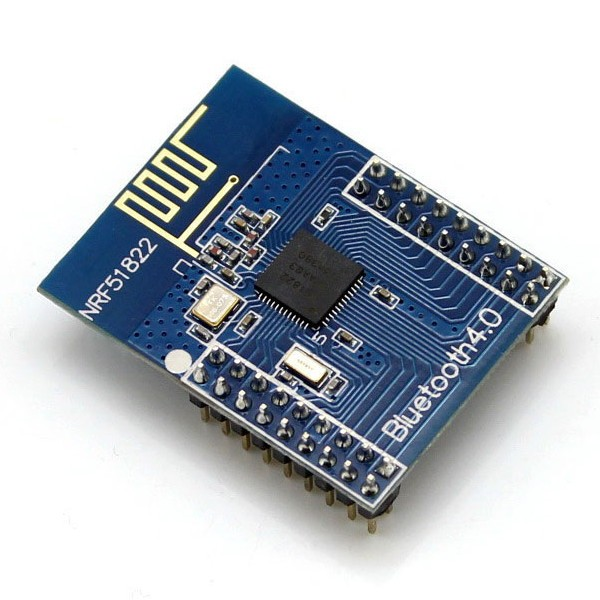
\includegraphics[width=0.7\textwidth]{img/board.jpg}
\caption{Moduł BLE z procesorem nRF51}
\label{fig:plytka}
\end{figure}

\subsubsection{Oprogramowanie znacznika radiowego}
W implementacji oprogramowania znacznika zrealizowano następujące funkcjonalności:
\begin{itemize}
 \item praca w trybie rozgłoszeniowym z interwałem 100 ms,
 \item zawartość pakietu rozgłoszeniowego pozwalająca odróżnić beacon systemu od ewentualnych innych urządzeń BLE w okolicy,
 \item zawartość pakietu rozgłoszeniowego pozwalająca rozróżnić poszczególne beacony wchodzące w skład systemu,
 \item możliwość konfiguracji zawartości pakietu rozgłoszeniowego za pomocą aplikacji mobilnej.
\end{itemize}

Należy zaznaczyć, że zasadnicza funkcjonalność znacznika tj. przekazywanie siły sygnału RSSI jest dostępna dla każdej konfiguracji rozgłaszania, ponieważ jest elementem wbudowanym w stos Bluetooth.

Tabela \ref{tab:adv} opisuje strukturę pakietu rozgłoszeniowego znacznika. Specyfikacja protokołu BLE przewiduje, że w ramce rozgłoszeniowej znajdą się pola reprezentujące poszczególne informacje \cite{ble}. Pole składa się z 2 + N bajtów: pierwszy bajt zawiera długość pola, drugi określa typ informacji, pozostałe zawierają daną informację. Łączny rozmiar wszystkich pól nie może przekroczyć 31 bajtów. Należy także nadmienić, że do długości pola wlicza się bajt typu. Specyfikacja przewiduje typy takie jak nazwa, klasa urządzenia, lista dostępnych serwistów itp.

W ramce znacznika wykorzystano następujące typy (por. tab. \ref{tab:adv}): 
\begin{description}
 \item[Flagi] - pole to jest obowiązkowe w każdej ramce. Zawiera jednobajtowe pole bitowe z flagami określającymi m.in. widoczność urządzenia.
 \item[Nazwa] - pole to zawiera nazwę urządzenia, wyświetlaną przez urządzenia nasłuchujące rozgłaszania (np. smartfon). Nazwa urządzenia to ,,locationTAG''
 \item[Zawartość producenta] - pole to jest przeznaczone do dowolnego wykorzystania przez producenta urządzenia. Zawarto w nim główną informacyjną treść ramki.
\end{description}

Pole ``Zawartość producenta'' zawiera następujące informacje (por. tab. \ref{tab:adv}):
\begin{description}
 \item[Kod producenta] - obowiązkowy kod producenta. Dla producentów niezarejestrowanych w Bluetooth SIG jego wartość wynosi FFFFh
 \item[Identyfikator grupy] - 4-bajtowa liczba całkowita (unsigned int32), służąca do odróżniania grup beaconów (np. zebranych w jednym pomieszczeniu)
 \item[Identyfikator znacznika] - 6-bajtowy identyfikator indywidualny dla znacznika. Jest on równy adresowi fizycznemu MAC znacznika. 
\end{description}


\begin{table}[]
\centering
\caption{Struktura pakietu rozgłoszeniowego}
\label{tab:adv}
\begin{tabular}{|l|l|l|l|l|l|l|l|l|l|l|l|}
\hline
\multicolumn{12}{|c|}{\centering Ramka rozgłoszeniowa [31B]}                                                                                                                         \\ \hline
\multicolumn{3}{|c|}{Flagi [3B]} & \multicolumn{3}{c|}{Nazwa [13B]} & \multicolumn{6}{c|}{Zawartość [15B]}                                                 \\ \hline
\rotatebox{90}{ \textit{Długość} [1B]}   & \rotatebox{90}{\textit{Typ} [1B]}  & \rotatebox{90}{Flagi [1B]}   & \rotatebox{90}{ \textit{Długość} [1B]}      & \rotatebox{90}{\textit{Typ} [1B]}    & \rotatebox{90}{Nazwa [11B]}    & \rotatebox{90}{ \textit{Długość} [1B]}  & \rotatebox{90}{\textit{Typ} [1B]} & \rotatebox{90}{Kod producenta [2B]} & \rotatebox{90}{Identyfikator grupy [4B]} & \rotatebox{90}{Identyfikator znacznika [6B]} & \rotatebox{90}{Wyrównanie [1B]} \\ \hline
\end{tabular}
\end{table}

\subsection{Robot}
W projekcie wykorzystano robota Pioneer 3-AT, będącego na wyposażeniu Laboratorium Robotyki Mobilnej Instututu Automatyki i Robotyki (rys \ref{fig:robot}). Jest to czterokołowy robot o napędzie różnicowym, zaprojektowany jako platforma edukacyjna z szerokimi możliwościami dalszej rozbudowy. Robot w laboratorium został wyposażony w komputer jednopłytkowy Nvidia Jetson TK1, charakteryzujący się dużą mocą obliczeniową i wsparciem przetwarzania równoległego dzięki technologii CUDA. Komputer działa pod kontrolą systemu operacyjnego Ubuntu Linux i wykorzystuje platformę ROS.

Komputer jest połączony z niskopoziomowymi sterownikami sensorów oraz aktuatorów robota za pomocą interfejsu szeregowego RS-232. Ponadto robot posiada kartę Intel Wireless-AC 7260, zapewniającą łączność Wi-Fi oraz Bluetooth, w tym także Bluetooth Low Energy. Układ sensoryczny robota obejmuje enkodery kół, sonar, kamerę USB oraz skaner laserowy Hokuyo URG-04LX-UG01. Do teleoperacyjnego sterowania robotem wykorzystywany jest kontroler z konsoli do gier Xbox \cite{daniel}.

\begin{figure}
\centering
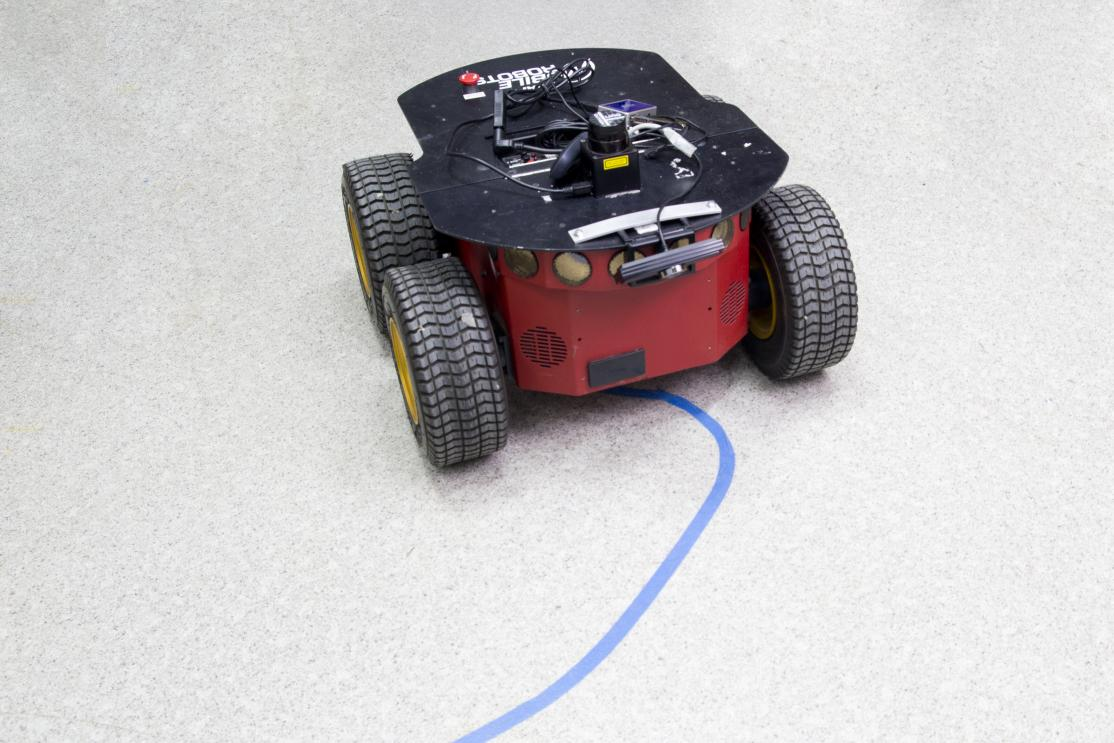
\includegraphics[width=0.7\textwidth]{img/robot.jpg}
\caption{Robot Pioneer 3-AT \cite{daniel}}
\label{fig:robot}
\end{figure}

\section{Oprogramowanie}
Ponieważ robot Pioneer, jak wspomniano powyżej, działa pod kontrolą systemu ROS, zdecydowano zaimplementować oprogramowanie nasłuchujące jako aplikacje ROS. 

ROS umożliwia pisanie aplikacji w trzech językach programowania \cite{roswiki} \cite{learning_ros}: 
\begin{itemize}
 \item C++
 \item Python
 \item JavaScript (Node.js)
\end{itemize}

Język C++ pozwala na napisanie programu bardzo wydajnego obliczeniowo, ponieważ jest to język kompilowany. Jednakże przygotowanie programu i jego zmiany wymagają relatywnie dużego nakładu pracy. 
Język Python, jako język interpretowany, znacznie gorzej radzi sobie w zadaniach obliczeniowych, jednak programy są łatwiejsze do napisania i utrzymania ze względu na prostą składnię, wysokopoziomowość i bogaty zasób bibliotek. Język JavaScript podobnie jak Python, ma przeciętną wydajność obliczeniową. Jednak biblioteki ROS w języku JavaScript zostały zaimplementowane stosunkowo niedawno i można się spodziewać, że zbiór bibliotek jest niekompletny lub niestabilny. 

Ostatecznie, do implementacji aplikacji nasłuchującej wybrano język Python. Wydajność obliczeniowa nie jest problemem, ponieważ aplikacja nie wykonuje żadnych złożonych obliczeń na dużych zbiorach danych. Natomiast elastyczność języka Python pozwoliła na zaprojektowanie aplikacji w taki sposób, aby możliwe było łatwe jej modyfikowanie i rozszerzanie, przy relatywnie niewielkim nakładzie pracy. 


\subsection{Gromadzenie danych ze znaczników}
Gromadzenie danych ze znaczników radiowych jest zadaniem aplikacji nasłuchującej. Nasłuch sensu stricto jest realizowane przez sterowniki stosu Bluetooth systemu operacyjnego. Jednakże zastosowanie danych ze znaczników do lokalizacji wymaga postawienia pewnych dodatkowych założeń:
\begin{itemize}
 \item \textit{Nasłuch ciągły} - większość interfejsów do sterowników Bluetooth udostępnia możliwość skanowania w poszukiwaniu rozgłaszających beaconów przez pewien określony czas, po czym skanowanie jest przerywane. Tymczasem system lokalizacji wymaga, aby skanowanie przeprowadzać w sposób ciągły. Optymalnie, powinno być możliwe przechwycenie każdego pakietu rozgłoszeniowego.
 \item \textit{Filtrowanie urządzeń} -  w środowisku pracy systemu potencjalnie mogą się znaleźć inne urządzenia BLE. Aplikacja nasłuchująca powinna je odfiltrować.
 \item \textit{Interfejsy do dalszego przetwarzania} - zebrane w postaci pakietów rozgłoszeniowych dane powinny być udostępnione do dalszego przetwarzania poprzez odpowiedni interfejs.
\end{itemize}

\subsubsection{Integracja z API Bluetooth}
Ponieważ oprogramowanie ROS działa w systemie operacyjnym Linux, konieczne jest zintegrowanie aplikacji ROS ze sterownikiem Bluetooth.  W większości dystrybucji systemu Linux, Bluetooth działa pod kontrolą stosu BlueZ, będącego oficjalną implementacją stosu Bluetooth dla systemów Linux. 

Do integracji aplikacji w języku Python z API Bluetooth konieczne jest zastosowanie dodatkowej biblioteki. Ponieważ implementacja takiej biblioteki jest zadaniem złożonym i wykraczającym poza zakres niniejszej pracy, wykorzystano bibliotekę bluepy autorstwa Iana Harvey'a. Biblioteka ta stanowi interfejs API BlueZ w języku C do języka Python \cite{pybluez}.

\subsubsection{Architektura aplikacji nasłuchującej}
Tor przetwarzania aplikacji rozłożony jest na dwa wątki wymieniające dane za pomocą chronionej struktury danych. 

API biblioteki BlueZ jest zaprojektowane jako synchroniczne. Oznacza to, że funkcja odpowiedzialna za wykonanie skanowania BLE zwraca dopiero po zakończeniu skanowania. Dlatego, aby zapewnić responsywność programu, skanowanie jest uruchamiane w oddzielnym wątku. Funkcja jest wywoływana w pętli, wykonując skanowanie o zadanej długości. Pętla może być przerwana przez odpowiednią funkcję i wtedy wątek kończy pracę. 
Każde znalezione podczas skanowania urządzenie jest dodawane do kontenera. Kontener jest oparty na mapie (w języku Python nazywanej słownikiem, ang. \textit{dictionary}), w której kluczem jest adres fizyczny MAC beacona, zaś wartością - obiekt przechowujący informacje odebrane z rozgłaszania. Kontener został wzbogacony o dwa dodatkowe mechanizmy: 
\begin{itemize}
 \item \textit{Usuwanie starych wpisów} - wpisy, reprezentujące pakiety rozgłoszeniowe, starsze niż zadana wartość mogą zostać usunięte z kontenera.
 \item \textit{Ochrona dostępu} - dla zapewnienia bezpiecznej synchronizacji między wątkami, każdy dostęp do danych w kontenerze (odczyt, pobranie całej zawartości, dodanie nowego wpisu) jest chroniony za pomocą obiektu \textit{Lock}, zapewniającego atomowość dostępu.
\end{itemize}

W wątku głównym programu prowadzone jest publikowanie wiadomości zawierających dane rozgłoszeniowe. W tym celu aplikacja wykorzystuje obiekt opakowujący klasę \textit{Publisher} biblioteki ROS \cite{agitr}. Jego rolą jest odfiltrowanie urządzeń nienależących do systemu oraz posiadających nieprawidłowy identyfikator grupy (por. \ref{subsec:znacznik}). 

Ustalono, że wszystkie aplikacje systemu będą działać w przestrzeni nazw składającej się z nazwy robota oraz członu \textit{beacon{\_}localization}. Aplikacja nasłuchująca działa pod nazwą \textit{beacon{\_}listener}. Znalezione urządzenia są publikowane do tematu o nazwie \textit{location{\_}tag}. 

\subsection{Filtracja i konwersja danych RSSI na odległość}
\label{subsec:filtracja_rssi}

Jak wspomniano w rozdziale \ref{ch:radio}, wartość siły sygnału RSSI podlega wahaniom nawet w wypadku, gdy nadajnik i odbiornik są nieruchome względem siebie. Ponadto, wahania wartości są dość duże, rzędu 5 dBm. Takie wahanie przekładałoby się bezpośrednio na wahanie przeliczonej odległości i znacznie osłabiało jakość lokalizacji. Dlatego konieczne jest wprowadzenie filtracji wartości siły sygnału, takiej, aby wahania stanu stacjonarnego zostały wygładzone. Jednocześnie bezwładność wprowadzana przez filtr nie może być zbyt duża, ponieważ odbiłoby się to negatywnie na lokalizacji podczas ruchu robota. 

Filtracja i konwersja na odległość jest realizowana przez oddzielną aplikację ROS, noszącą nazwę \textit{rssi2distance}. Aplikacja ta subskrybuje temat \textit{location{\_}tag}, zaś przefiltrowane i skonwertowane dane publikuje w tematach \textit{distances/}$<$nazwa filtra$>$ . Ten sam wynik działania aplikacji jest dostępny również za pomocą usługi ROS działającej pod tą samą nazwą. Dane wynikowe są publikowane w postaci tablicy, zawierającej wszystkie znaczniki radiowe będące aktualnie w zasięgu, łącznie z przefiltrowaną wartością RSSI, przeliczoną odległością oraz pozycją znacznika w układze współrzędnych mapy pomieszczenia.

\subsubsection{Filtracja}
Zaimplementowano następujące filtry (kursywą podano nazwy filtrów używane do nazywania wynikowych tematów i usług):
\begin{enumerate}
 \item \textit{recent} - brak filtra. Filtr zwraca najnowszą znaną wartość RSSI. Jest to najprostsza strategia, używania głównie do testów podczas rozwoju oprogramowania.
 \item \textit{moving{\_}average} - średnia krocząca. Filtr zwraca średnią kroczącą prostą z 5 ostatnich pomiarów:
      \begin{equation}
       \bar P_{k} = \frac{ P_{k} + P_{k-1} + \cdots + P_{k-4} }{5}
      \end{equation}
 \item \textit{probabilistic} - prosty filtr probabilistyczny. Opiera się on na założeniu, że zmiana odległości od znacznika ze stałą prędkością będzie skutkować stałą zmianą wartości RSSI. Działanie filtra można podzielić na fazy estymacji i predykcji \cite{trilat_iter}. Równania estymacji:
 \begin{equation}
  \hat P_{est k } = \hat P_{pred k } + a (P_{k } - \hat P_{pred k })
 \end{equation}
 \begin{equation}
  \hat V_{est k } = \hat V_{pred k } + \frac{b}{T_s} (P_{k } - \hat P_{pred k })
 \end{equation}
 Równania predykcji:
 \begin{equation}
  \hat P_{pred \{k+1\} } = \hat P_{est k } + \hat V_{est k } T_s
 \end{equation}
 \begin{equation}
  \hat V_{pred \{k+1\} } = \hat V_{est k }
 \end{equation}
 
  W powyższych równaniach $\hat P_{est k }$ jest wynikiem działania filtra - wygładzoną wartością RSSI, $V_{est k }$ i $V_{pred k }$ to wartość estymowanego tempa zmiany RSSI, $a$ i $B$ są stałymi strojącymi filtr, zaś $T_s$ jest okresem próbkowania RSSI. 

\end{enumerate}

\subsubsection{Konwersja RSSI na odległość}
Model propagacji, służący do przeliczania RSSI na odległość, również został zaimplementowany na podstawie wzorca Strategii. Model realizuje równanie \ref{eq:logfit_d}.

\subsubsection{Mapa znaczników}
Mapa znaczników jest publikowana przez dodatkową aplikację o nazwie \textit{beacon{\_}tf{\_}publisher}. Pobiera ona konfigurację mapy w postaci koordynatów i odpowiadających im identyfikatorów znacznika z pliku YAML, następnie publikuje w postaci transformacji z układu współrzędnych mapy do układów poszczególnych znaczników, wykorzystując bibliotekę \textit{tf}. 


\subsection{Trilateracja}
Dysponując oprogramowaniem do zbierania danych ze znaczników i konwersji siły sygnału RSSI na odległość, przystąpiono do projektowania właściwych aplikacji lokalizujących. Pierwsza z nich wykorzystuje technikę trilateracji. 
Strukturę aplikacji rozwiązującej zadanie trilateracji oparto na pętli wykonującej się z określonym interwałem. W każdej iteracji wykonywane jest zapytanie do usługi ROS udostępnianej przez aplikację \textit{rssi2distance}. W odpowiedzi otrzymywana jest lista znaczników znajdujących się w zasięgu, wraz z przefiltrowaną wartością RSSI, przeliczoną wartością odległości i pozycją znacznika w układzie mapy. Możliwy jest wybór metody filtracji za pomocą odpowiedniego parametru na serwerze parametrów ROS. 

Jeśli w danej iteracji w zasięgu znajdowało się co najmniej trzy znaczniki, wykonywane jest rozwiązanie zadania trilateracji. Dostępne są dwie, bardzo zbliżone metody trilateracji:
\begin{enumerate}
 \item \textit{metoda Newtona} - opisana w rozdziale \ref{sec:trilateracja}
 \item \textit{metoda L-BFGS (Limited-Memory Broyden–Fletcher–Goldfarb–Shanno } - jest to metoda minimalizacji należąca do rodziny metod quasi-Newtonowskich, implementowana przez bilbiotekę \textit{scipy}
\end{enumerate}
Metoda trilateracji również może być wybierana za pomocą serwera parametrów. 

Wynik obliczeń jest konwertowany na wiadomość typu \textit{geometry{\_}msgs/Pose}), reprezentującą pozycję i orientację obiektu w przestrzeni trójwymiarowej. Jest to typowa konwencja w systemie ROS, nawet jeśli lokalizacja ogranicza się do dwóch wymiarów. Wynik jest publikowany w temacie \textit{beacon{\_}localization/bl{\_}pose} oraz jako transformacja z układu mapy do układu robota. 


\section{Filtr cząsteczkowy}
Ponieważ algorytm trilateracji wykorzystuje tylko dane ze znaczników, jest wrażliwy na zakłócenia wynikłe z ich działania, np. rozrzut wartości RSSI w stanie ustalonym. Dlatego następnym krokiem było zaprojektowanie aplikacji lokalizującej robota w oparciu nie tylko o dane ze znaczników, ale także z sensorów odometrycznych. W celu zintegrowania tych danych wykorzystano filtr cząsteczkowy, co do teorii opisany w rozdziale \ref{sec:filtr-czasteczkowy}.
Filtr cząsteczkowy zaimplementowano w oparciu o implementację autorstwa Dakoty Nelsona dostępną na licencji MIT. Źródłowa implementacja dotyczyła filtra cząsteczkowego wykorzystującego skaner laserowy oraz sensor odometryczny. Aplikacja subskrybuje do tematu \textit{distances/}$<$nazwa filtra$>$, gdzie publikowane są tablice znajdujących się w zasięgu znaczników, wraz z ich pozycjami na mapie. Aby ograniczyć obciążenie komputera obliczeniami, algorytm filtra jest wykonywany tylko jeśli przemieszczenie kątowe lub liniowe robota wynikłe z pomiaru odometrycznego przekroczyło pewien konfigurowalny próg. Jako metodę resamplingu wykorzystano algorytm SRR (\textit{Sequential Random Resampling}, ang. sekwencyjny losowy resampling) \cite{jupyter}.
\clearpage{\pagestyle{empty}\cleardoublepage}

\chapter{Badania eksperymentalne} 
\label{ch:testy}



\section{Wykorzystane narzędzia}
Do rozwoju i testowania oprogramowania wykorzystano przede wszystkim narzędzia dostępne w systemie ROS. Przygotowano jednak także kilka dodatkowych narzędzi.

\subsubsection{RViz}
Program RViz (\textit{ROS Visualization}) jest należącym do systemu ROS narzędziem wizualizacji danych. Posiada szereg integracji, pozwalających m. in. na:
\begin{itemize}
 \item wyświetlanie mapy pomieszczenia wyznaczonej metodą SLAM lub inną,
 \item wyświetlanie układów współrzędnych i ich wzajemnych relacji (integracja z biblioteką \textit{tf}),
 \item subskrypcję i wizualizację niektórych typów wiadomośći dotyczących geometrii robota, m. in. \textit{Pose}, \textit{PoseWithCovariance},
 \item wizualizację danych ze skanera laserowego,
 \item interakcję z robotem np. poprzez zadawanie celu nawigacji.
\end{itemize}

\begin{figure}[H]
\centering
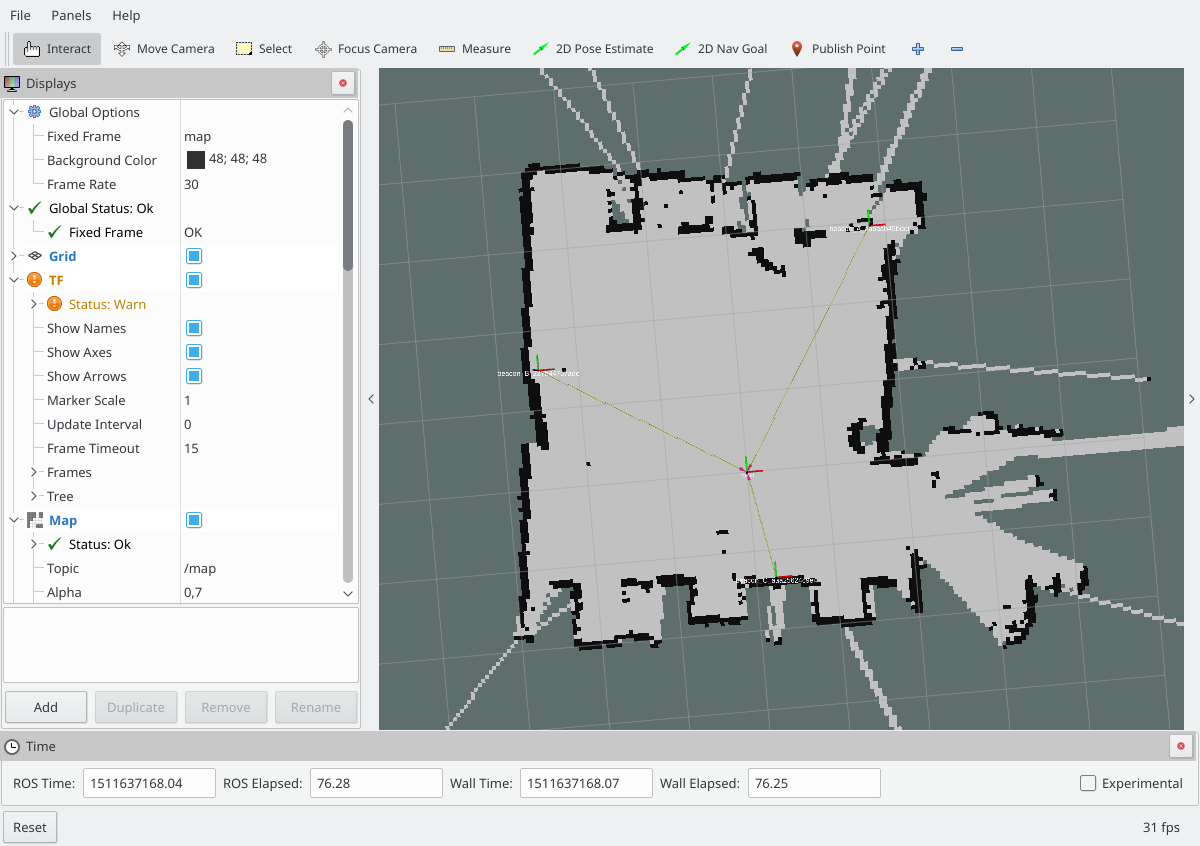
\includegraphics[width=0.8\textwidth]{img/rviz.png}
\caption{Okno programu RViz}
\label{fig:rviz}
\end{figure}

\subsubsection{Gmapping}
Gmapping jest narzędziem należącym do pakietu OpenSLAM, służącym do budowania dwuwymiarowych map pomieszczeń za pomocą SLAM (Simultaneous Localization And Mapping, ang. \textit{Jednoczesna Lokalizacja i Mapowanie}). Program wykorzystuje pomiar ze skanera laserowego oraz odometrię. 

\subsubsection{Rosbag}
Program Rosbag pozwala na zapisywanie do pliku danych publikowanych w wybranych tematach wraz z ich znacznikami czasowymi, celem późniejszego odtworzenia. Narzędzie to pozwoliło na nagranie szeregu testowych przejazdów robota, celem późniejszego zbudowania mapy pomieszczenia i wykonania pomiarów. Zaawansowane funkcjonalności manipulowania zegarem systemu ROS pozwalają na integrowanie danych odtwarzanych za pomocą Rosbag z danymi generowanymi w czasie rzeczywistym.

\subsubsection{Dodatkowe skrypty}
W ramach testów systemu przygotowano także szereg dodatkowych skryptów w języku Python:
\begin{itemize}
 \item skrypt do zbierania danych RSSI do pliku tekstowego, celem dalszej obróbki,
 \item skrypt do dopasowania modelu \ref{eq:logfit_d} do danych pomiarowych.
\end{itemize}


\section{Zmienność wartości siły sygnału RSSI}
\label{sec:zmiennosc}
\subsection{Metodyka badań}
Przedmiotem niniejszego eksperymentu było zbadanie przebiegu wartości RSSI w czasie dla sytuacji, w której nadajnik i odbiornik są nieruchome. Dodatkowo, wyznaczono histogramy wartości RSSI celem aproksymowania dystrybucji prawdopobieństwa wartości RSSI. 

Wykorzystano znacznik opisany w rozdziale \ref{subsec:znacznik} oraz odbiornik Wi-Fi/Bluetooth Intel 7260, zamontowany w laptopie Lenovo Y50 działającego pod kontrolą systemu Linux Mint 18. 

Testy przeprowadzono w pomieszczeniu o wymiarach 1.5 x 20 m (korytarz).Pomieszczenie to charakteryzował wysoki poziom zakłóceń radiowych w paśmie ISM (liczne punkty dostępowe Wi-Fi i odbiorniki elektryczne). Znacznik radiowy i odbiornik znajdowały się na wysokości 70 cm nad podłogą. Przeprowadzono pomiar dla odległości 1 m i 5 m. Pomiar polegał na zebraniu 100 wartości siły sygnału RSSI. Tak zebrane dane obrazowano w postaci wykresu czasowego i histogramu. 

\subsection{Wyniki}

Z wykresów \ref{fig:rssi-1m} i \ref{fig:rssi-5m} widać, że siła sygnału RSSI waha się znacznie nawet dla stanu ustalonego. Amplituda wahań dla odległości 1 m jest średnio rzędu 7 dBm. Dla odległości 5 m jest znacznie większa, rzędu 7 m. Stanowi to poważną przeszkodę dla pomiaru odległości za pomocą RSSI - kumulują się bowiem dwa negatywne czynniki: po pierwsze zależność RSSI od odległości jest w zakresie powyżej 2 m niemal płaska, po drugie - występują duże wahania wartości RSSI, które w tym zakresie będą się przekładać na znaczne wahania odległości. 

Wykresy \ref{fig:rssi-1m-hist} i \ref{fig:rssi-5m-hist} zawierają histogramy wygenerowane z danych pomiarowych. Dla odległości 1 m rozkład wyników pomiarów jest zbliżony do Gaussowskiego, jednak dla 5 m obserwujemy wyraźną asymetrię w kierunku niższych wartości siły sygnału. Jest to wynik wymienionych w rozdziale \ref{ch:radio} zakłóceń, szczególnie wielokrotnych odbić od ścian pomieszczenia. Także szerokość rozkładu jest większa niż w wypadku odległości 1 m. 

\begin{figure}[H]
\centering
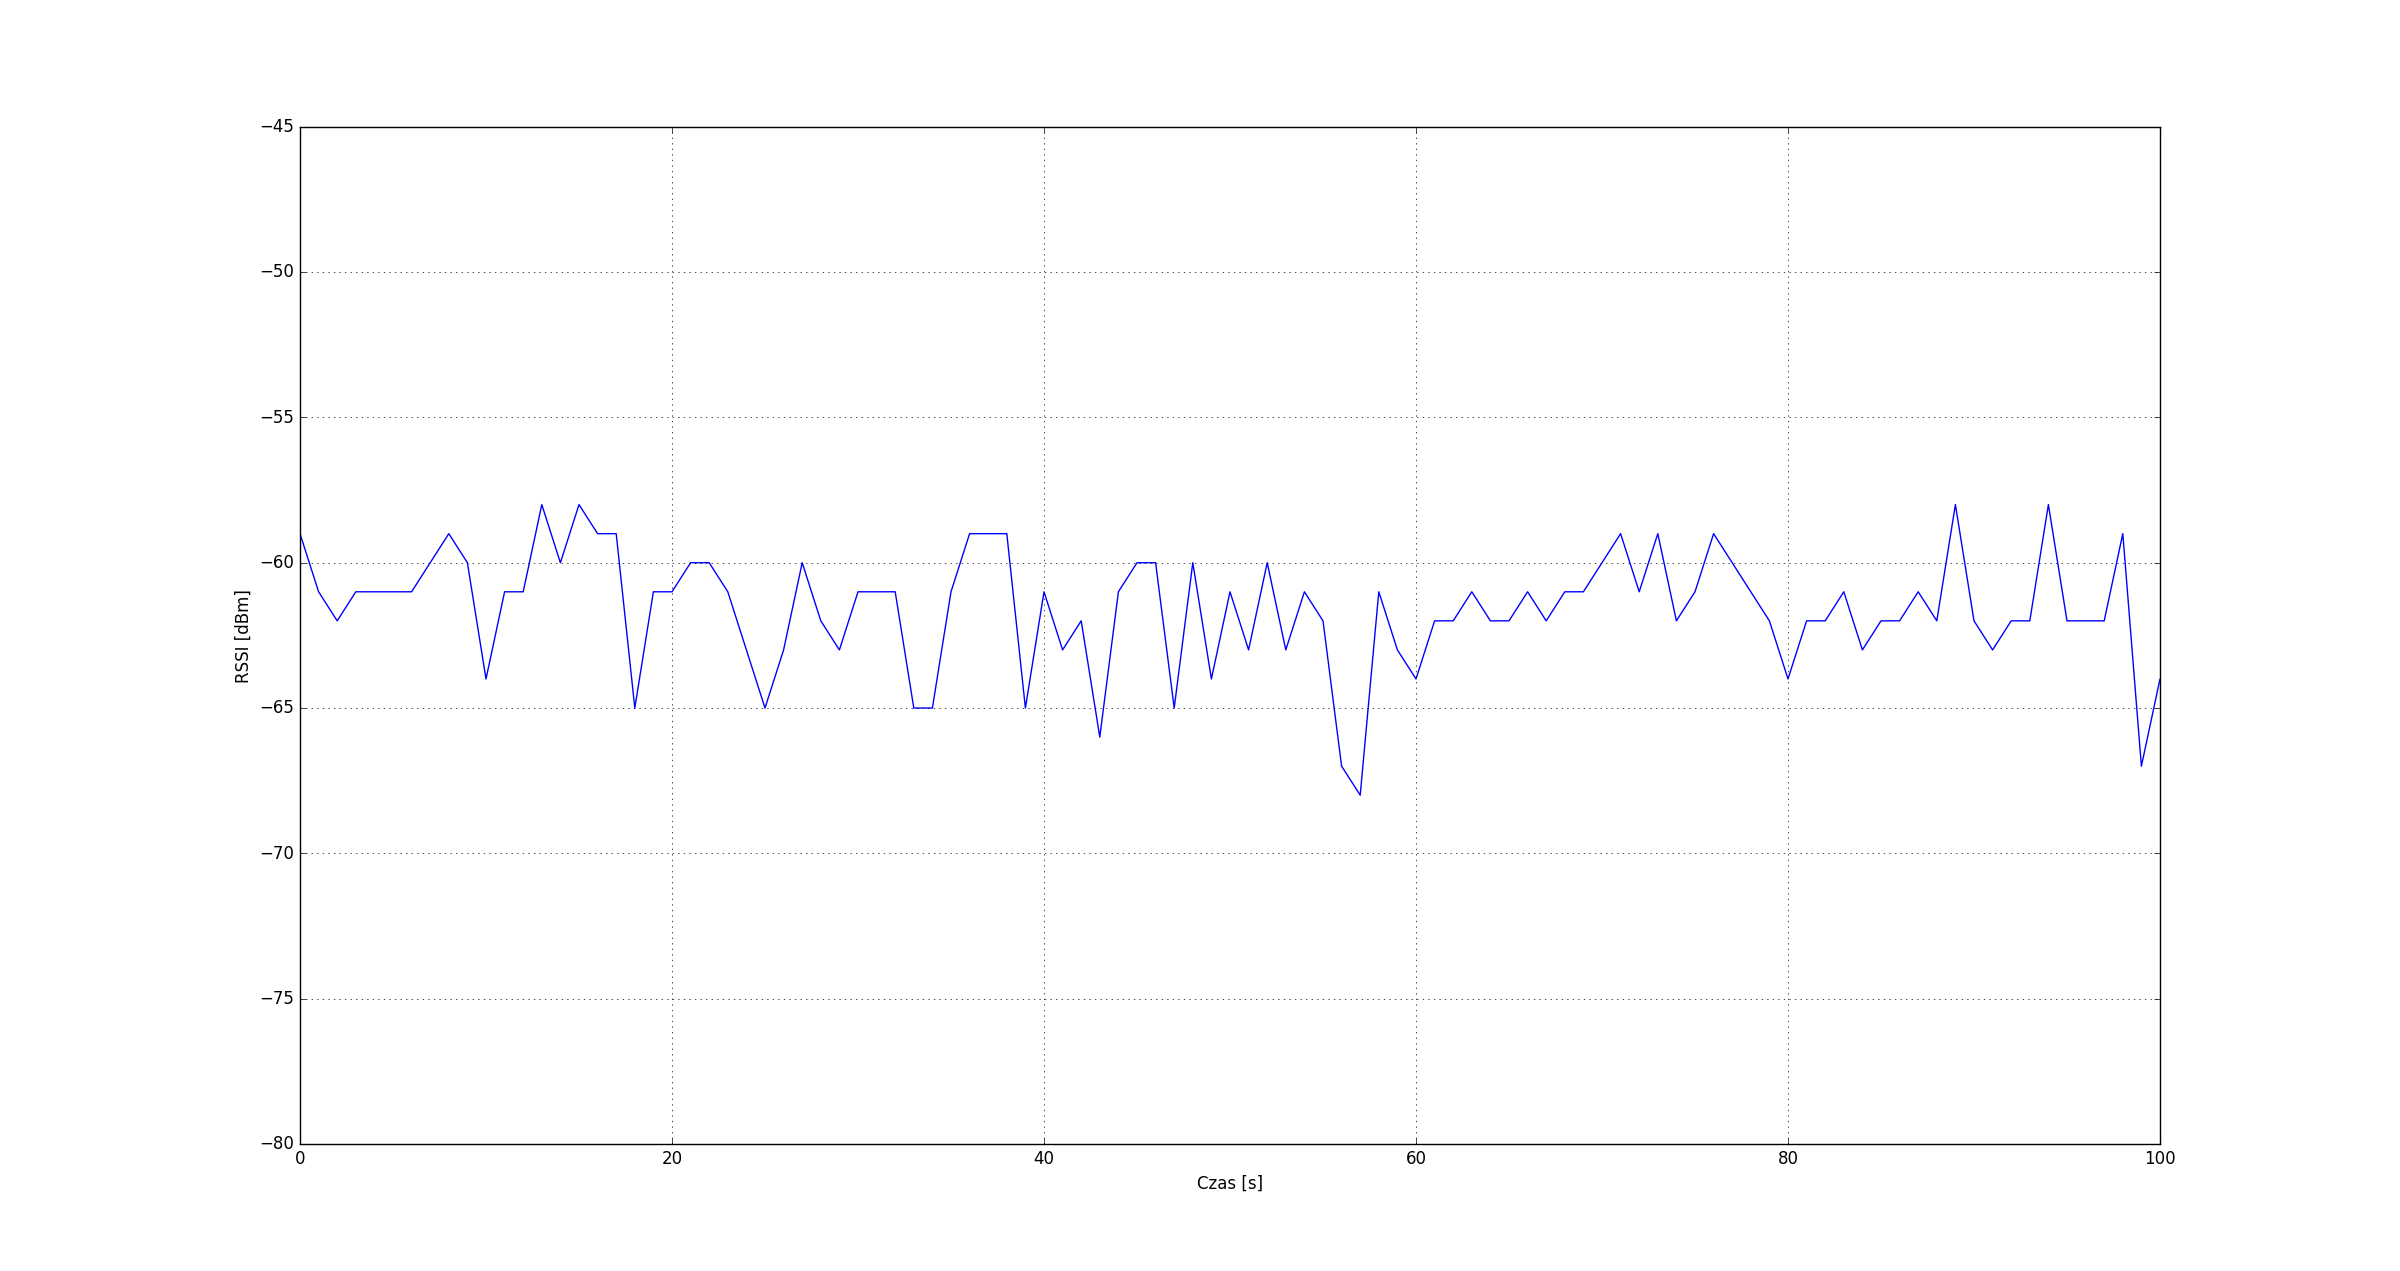
\includegraphics[width=1\textwidth]{img/1m.png}
\caption{Przebieg wartości siły sygnału RSSI w czasie dla odległości odbiornika od nadajnika równej 1 m}
\label{fig:rssi-1m}
\end{figure}

\begin{figure}[H]
\centering
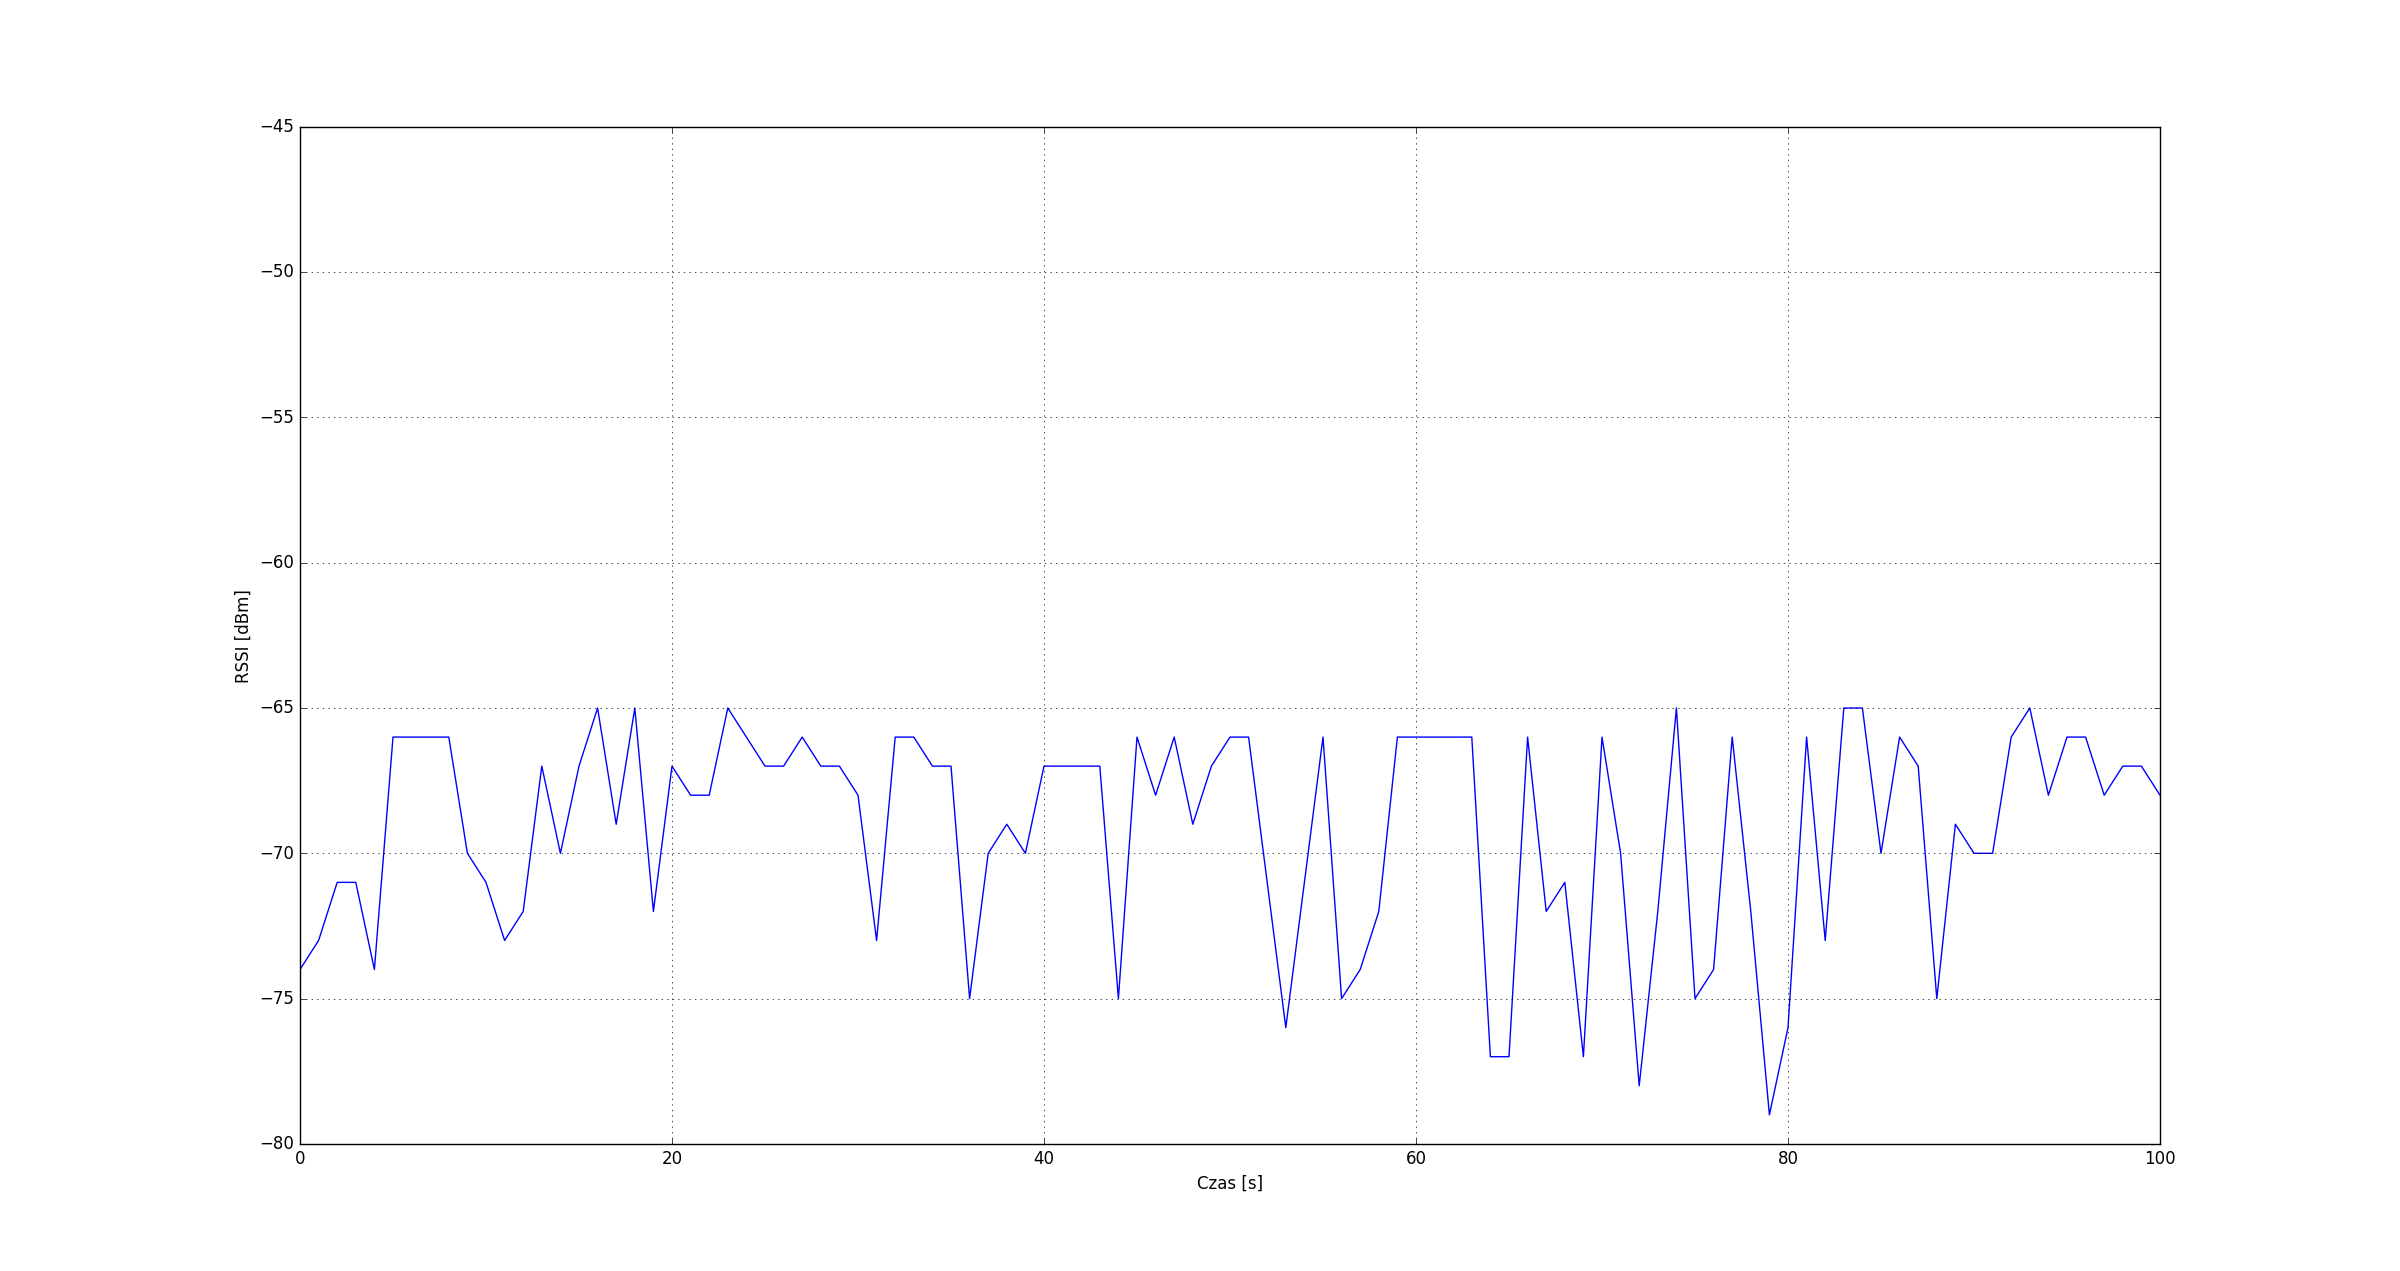
\includegraphics[width=1\textwidth]{img/5m.png}
\caption{Przebieg wartości siły sygnału RSSI w czasie dla odległości odbiornika od nadajnika równej 1 m}
\label{fig:rssi-5m}
\end{figure}

\begin{figure}[H]
\centering
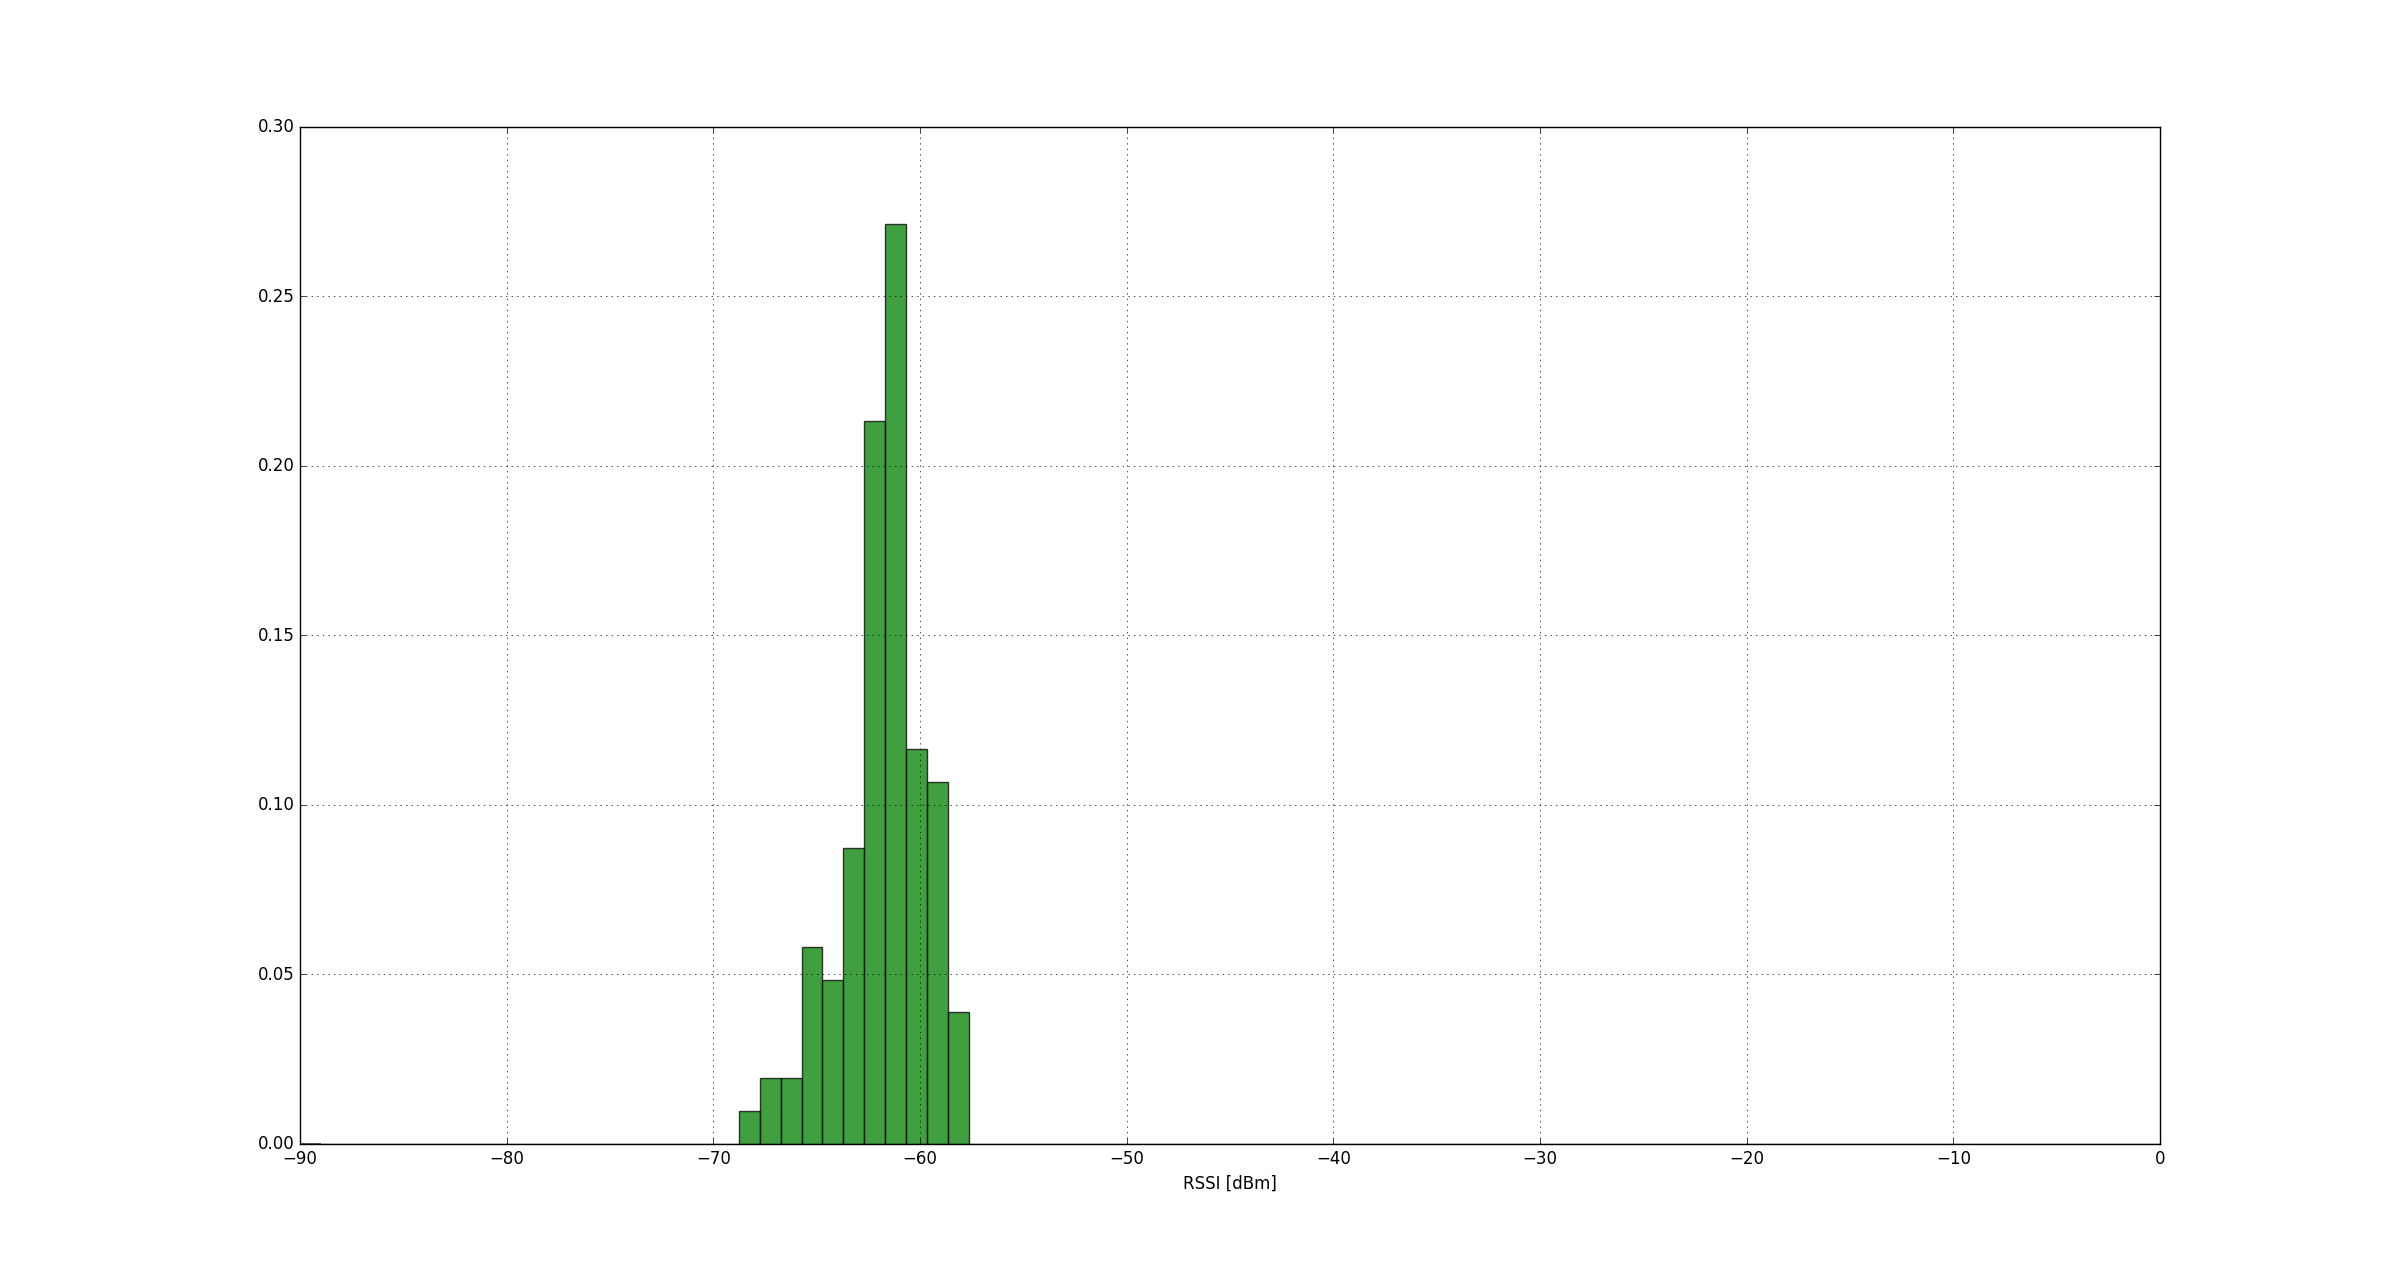
\includegraphics[width=1\textwidth]{img/1m-hist.png}
\caption{Histogram siły sygnału RSSI w czasie dla odległości odbiornika od nadajnika równej 1 m}
\label{fig:rssi-1m-hist}
\end{figure}

\begin{figure}[H]
\centering
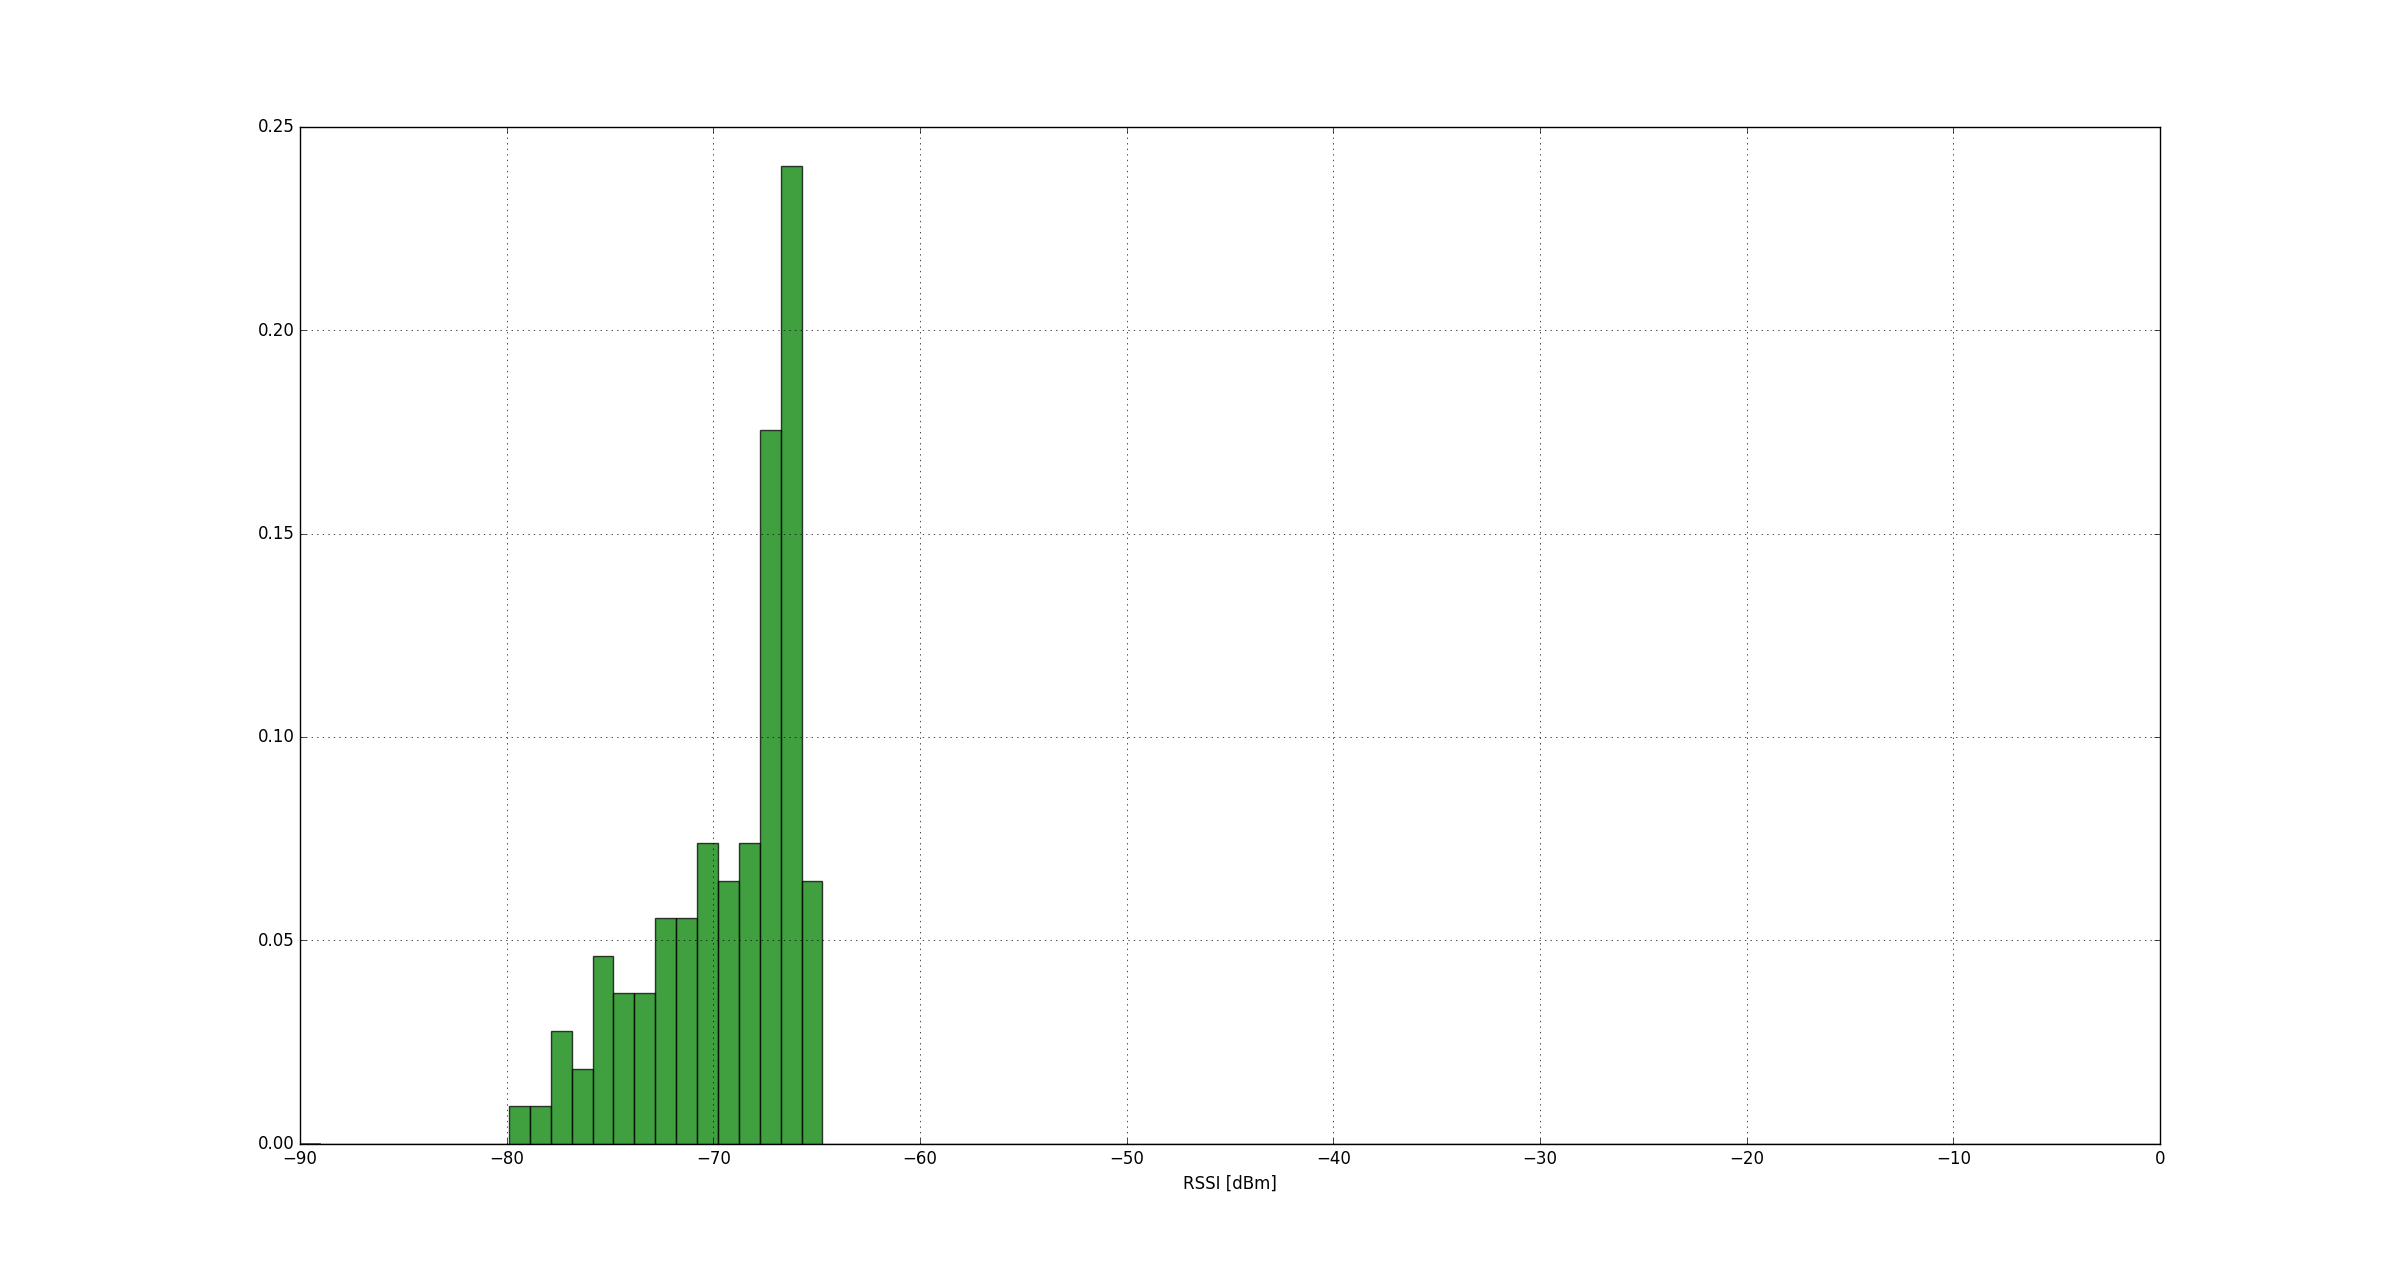
\includegraphics[width=1\textwidth]{img/5m-hist.png}
\caption{Histogram siły sygnału RSSI w czasie dla odległości odbiornika od nadajnika równej 1 m}
\label{fig:rssi-5m-hist}
\end{figure}


\section{Zależność siły sygnału RSSI od odległości}

\subsection{Metodyka badań}
Celem niniejszego eksperymentu jest zweryfikowanie modelu przedstawionego w rozdziale \ref{ch:radio}. Środowisko testowe było identyczne jak w punkcie \ref{sec:zmiennosc}. W każdym punkcie pomiarowym zebrano 30 próbek RSSI, które następnie uśredniono i wyznaczono odchylenie standardowe. Następnie wykonano dopasowanie krzywych logarytmicznych według metody interpolacji oraz dopasowania krzywej (por. rozdział \ref{sec:rssi-odleglosc}).

\subsection{Wyniki}

Na wykresie \ref{fig:odleglosc-rssi} widać logarytmiczną zależność pomiędzy odległością, a wartością siły sygnału RSSI, zgodną z oczekiwaniami teoretycznymi opisanymi w \ref{eq:model_propag}. Jednocześnie wraz ze wzrostem odległości od nadajnika, wzrasta odchylenie standardowe pomiarów, co oznacza że wahania wartości RSSI były większe. 

W odległości 3.5m oraz 5 m obserwujemy niewielki wzrost siły sygnału RSSI, co może wskazywać, że w tych miejscach środowiska testowego zachodziły warunki powodujące lokalne wzmocnienie fali. 
Należy zwrócić uwagę, iż w zakresie odległości powyżej 2 m wartość RSSI pozostaje na stałym poziomie, wahając się w granicach 10 dBm. Z tego powodu jakość pomiaru odległości za pomocą RSSI w tym zakresie będzie bardzo słaba. 

Wykres \ref{fig:odleglosc-rssi-fit} ukazuje dopasowane do wyników pomiaru krzywe: metodą interpolacji (\ref{eq:interpol}) i poprzez dopasowanie krzywej \ref{eq:logfit_d} za pomocą funkcji \textit{curve{\_}fit} z bilbioteki \textit{scipy} dla języka Python. Należy zwrócić uwage, iż w porównaniu z wykresem \ref{fig:odleglosc-rssi} zamienione zostały osie układu współrzędnych, tj. wykres \ref{fig:odleglosc-rssi-fit} przedstawia problem z perspektywy przeliczania RSSI na odleglość. 

Funkcja \textit{curve{\_}fit} uwzględnia wszystkie punkty pomiarowe wraz z ich niepewnościami, dlatego zapewnia lepsze dopasowanie od interpolacji, biorącej pod uwagę tylko dwa punkty pomiarowe. Jednakże, aby osiągnąć zadowalające dopasowanie, trzeba albo ręcznie wybrać dwa optymalne punkty do dopasowania interpolacyjnego, albo usunąć punkty zbyt odstające od pozostałych dla metody dopasowania krzywej. 

\begin{figure}[ht]
\centering
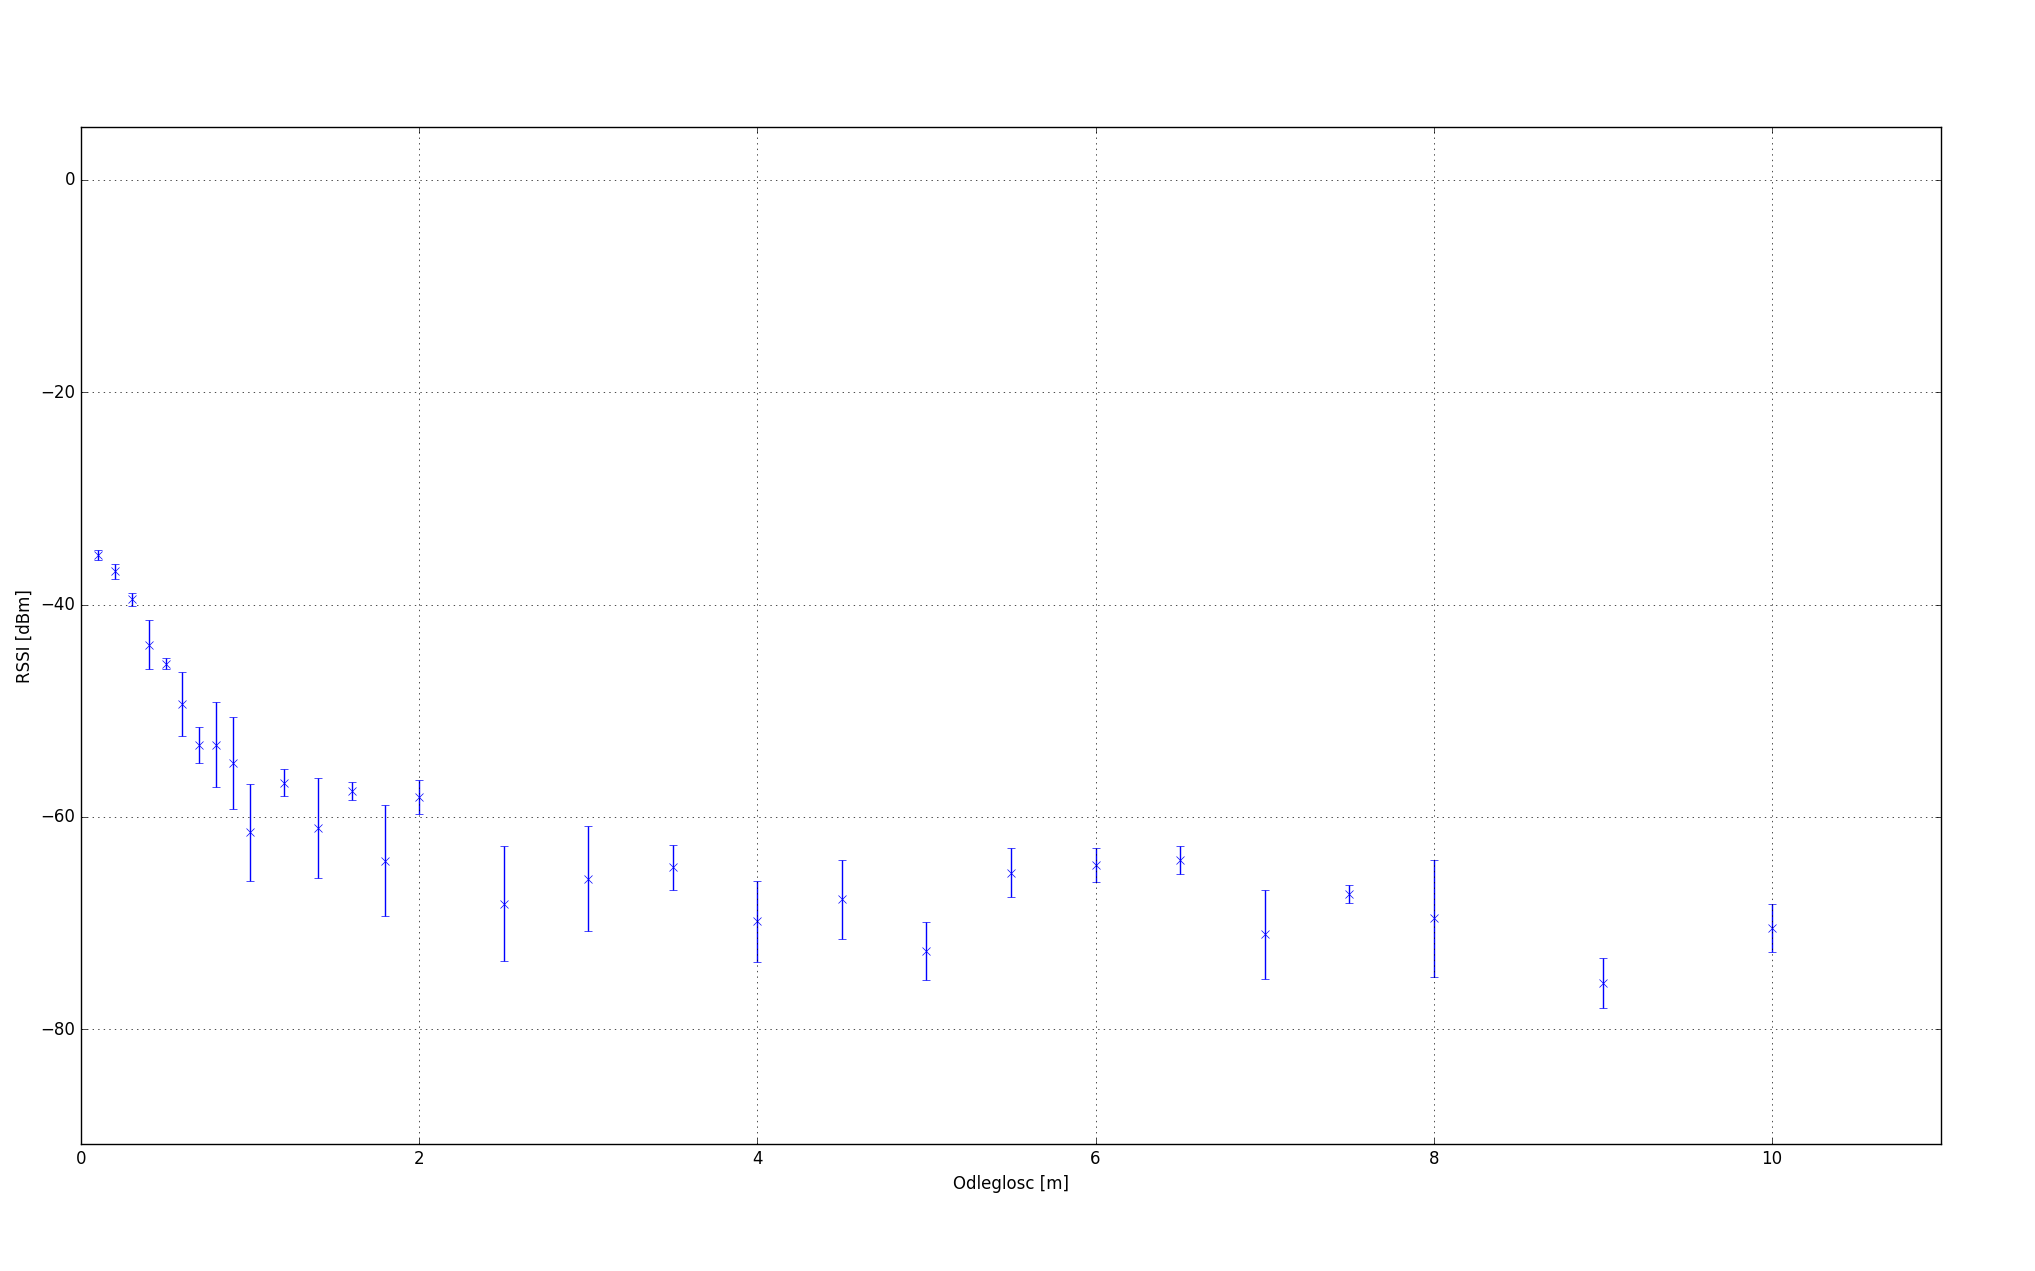
\includegraphics[width=1\textwidth]{img/odleglosc-rssi.png}
\caption{Wykres wartości siły sygnału RSSI w zależności odległości}
\label{fig:odleglosc-rssi}
\end{figure}


\begin{figure}[ht]
\centering
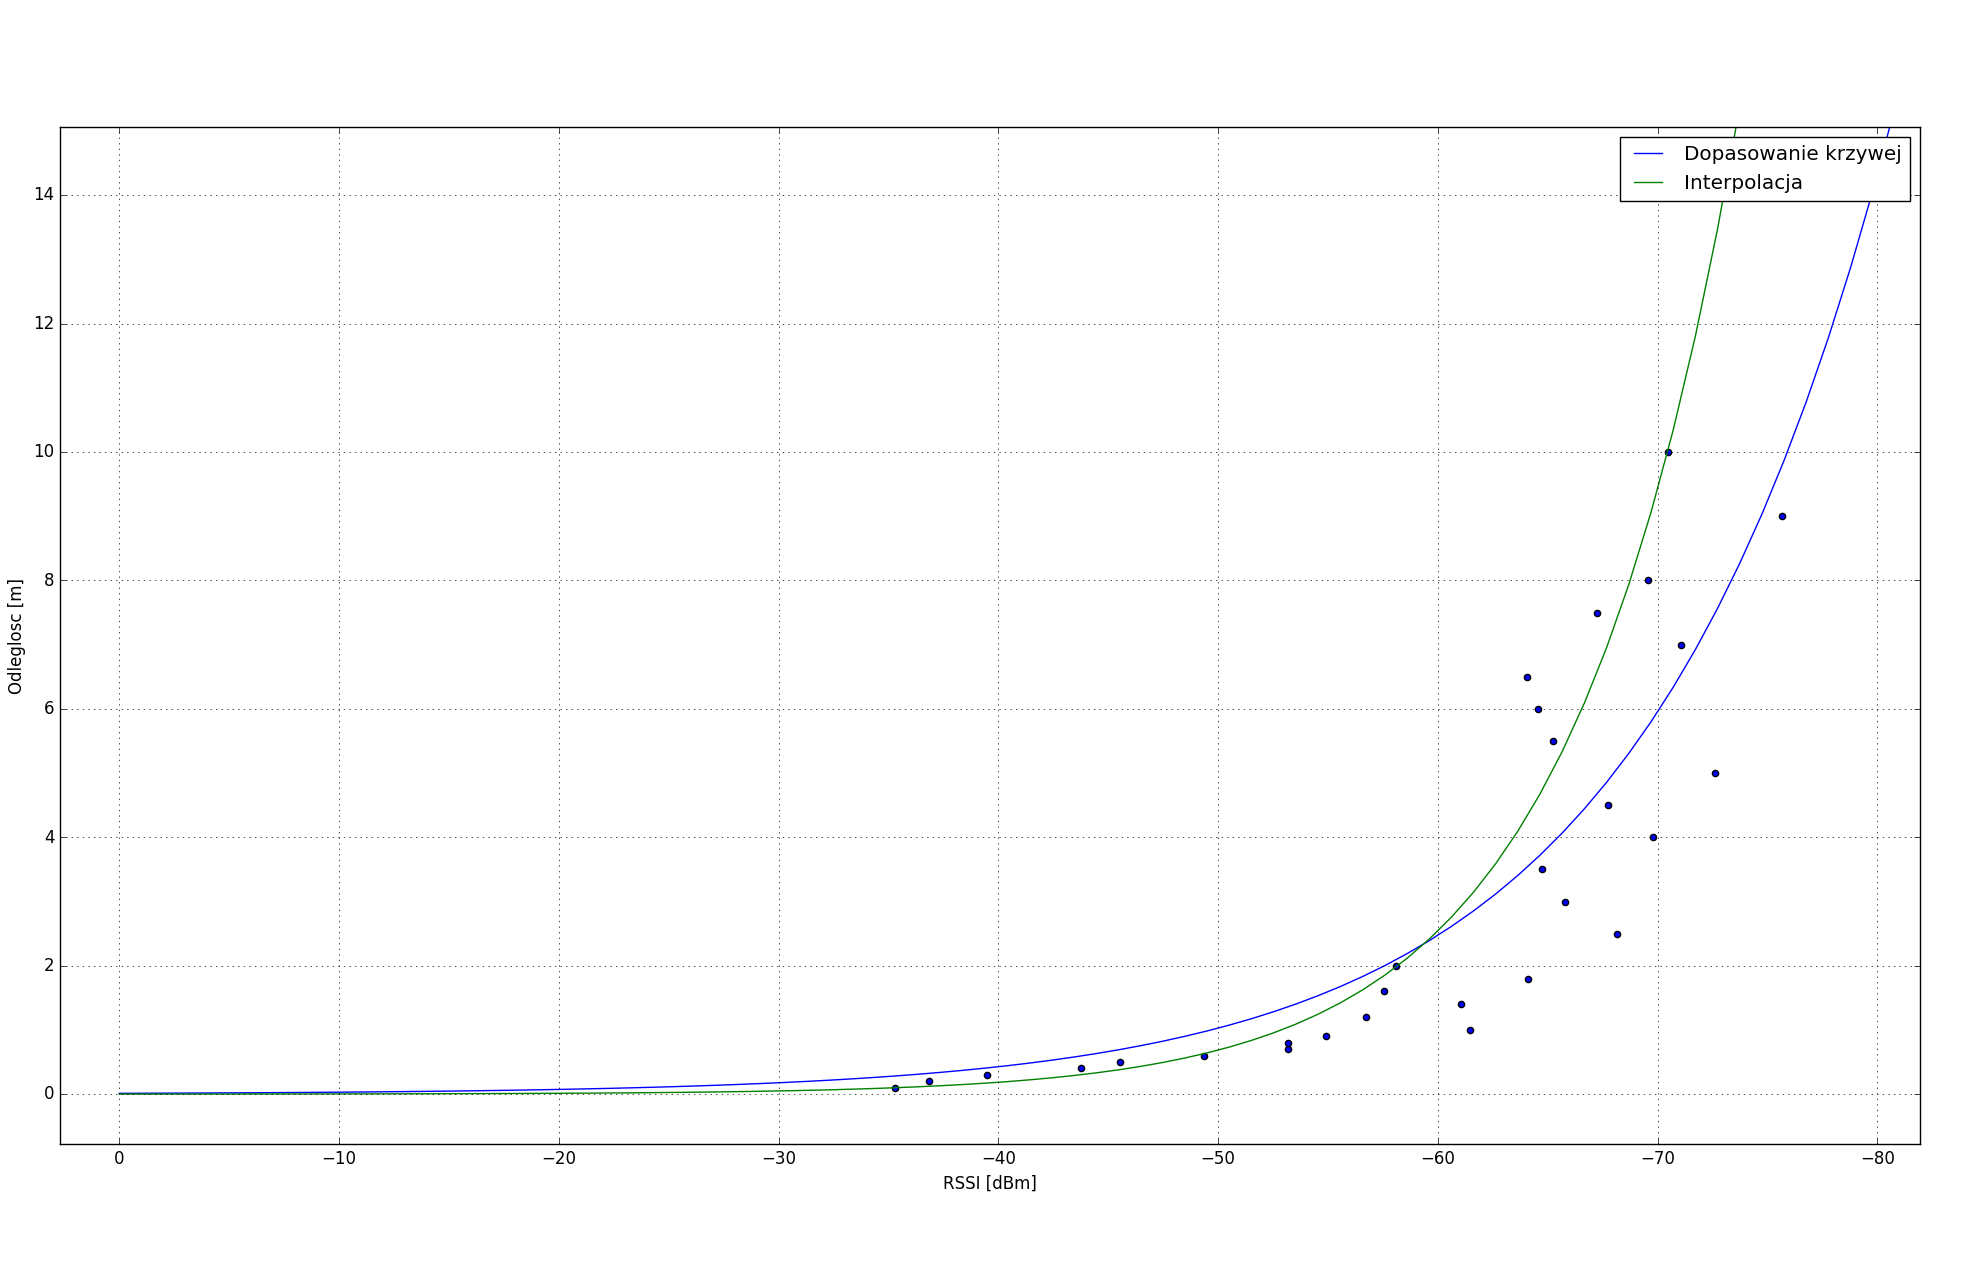
\includegraphics[width=1\textwidth]{img/rssi-odleglosc.png}
\caption{Wykres dopasowania krzywych potęgowych do wyników pomiaru}
\label{fig:odleglosc-rssi-fit}
\end{figure}

\section{Porównanie metod filtracji siły sygnału RSSI}
\label{sec:testy-filtracja}
\subsection{Metodyka badań}
Eksperyment miał na celu porównanie skuteczności metod filtracji sygnału RSSI opisanych w \ref{sec:rssi-odleglosc}. Pożądanym wynikiem jest dobre wygładzenie stacjonarnych wahań RSSI przy zachowaniu małej bezwładności, tj. szybkiej reakcji na rzeczywistą zmianę siły sygnału RSSI, wynikłą ze zmiany odległości od znacznika. 

W ramach eksperymentu posłużono się zbiorem danych nagranym za pomocą programu rosbag. Obejmował on pomiary RSSI zbierane z interwałem 1 sekundy, dla następującej sekwencji: przez 40 sekund znacznik pozostaje w odległości 1 m od odbiornika, następnie zostaje przeniesiony na odległość 2 m, po kolejnych 20 sekundach zostaje przeniesiony z powrotem na odległość 1 m gdzie pozostaje przez 40 sekund. 

\subsection{Wyniki}
Filtr średniej ruchomej (por. \ref{subsec:filtracja_rssi}) wprowadza znaczną bezwładność do układu (por. rys \ref{fig:filtry-avg}), przy czym dla większej liczby kroków średniej $N = 10$ bezwładność nie jest znacząco większa. Filtr zapewnia dobre wygładzenie dla nieruchomego odbiornika. W wypadku zmiany odgległości, filtr potrzebuje 10 sekund aby dość do stanu ustalonego, co dyskwalifikuje jego zastosowanie w lokalizacji dynamicznej. 

\begin{figure}[ht]
\centering
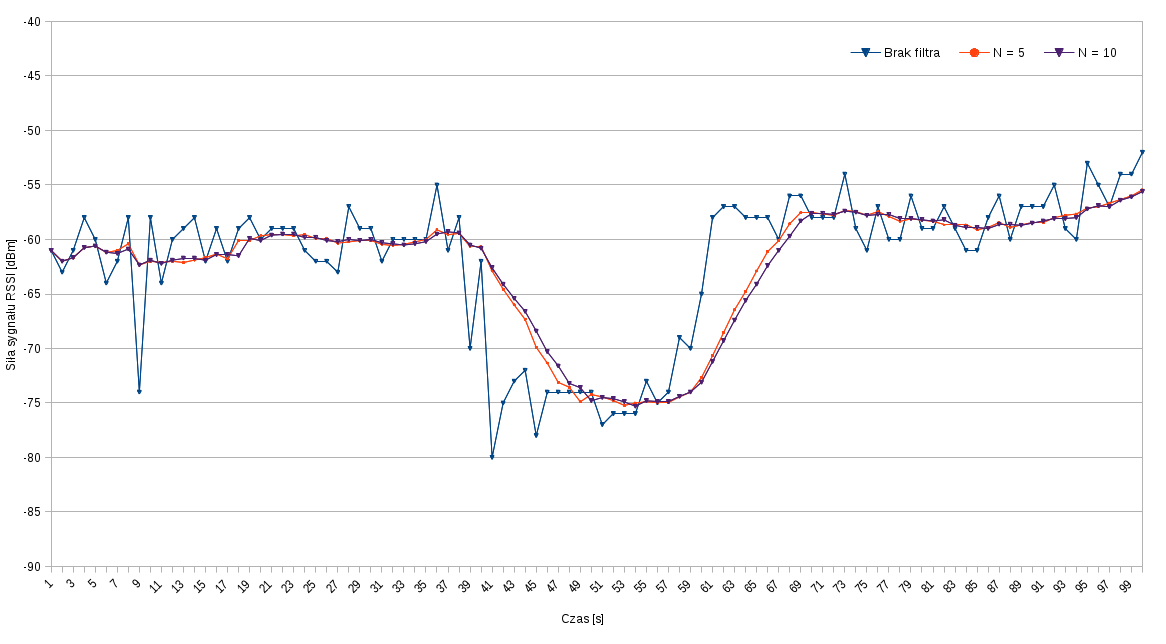
\includegraphics[width=0.9\textwidth]{img/filtr-avb.png}
\caption{Filtr średniej ruchomej}
\label{fig:filtry-avg}
\end{figure}

Filtr probablistyczny jest strojony za pomocą dwóch parametrów: $a$ - opisujący jak istotna jest wartość poprzedniego pomiaru w estymacji bieżącego, oraz $b$ - opisujący jak istotny jest przyrost wartości RSSI. Innymi słowy, parametr $a$ opisuje wygładzanie filtra, zaś $b$ opisuje czułość na zmiany RSSI. Zbyt niska wartość $a$ powoduje dużą bezwładność filtra, z kolei wartość $a=1$ powoduje że wartość estymowana jest wartości zmierzonej. Zbyt duża wartość $b$ spowoduje oscylacje, a nawet utratę stabilności filtra. 

W eksperymencie porównano dwa zestawy nastaw filtra (rys. \ref{fig:filtry-probab}):
\begin{itemize}
 \item \textbf{Nastawy 1} $a=0.35$ $b=0.02$
 \item \textbf{Nastawy 2} $a=0.15$ $b=0.005$
\end{itemize}

Nastawy 2 zapewniają dobre wygładzenie w stanie ustalonym oraz bardzo dużą bezwładność. Zwiększanie parametru $b$ spowoduje jedynie zaistnienie oscylacji, bez poprawy reakcji filtra. 

Z kolei nastawy 1 stanowią dobry kompromis pomiędzy wygładzeniem a reakcją na zmiany RSSI. Filtr reaguje na zmianę odległości w ciągu około 4 sekund, zaś amplituda wahań wartości w stanie ustalonym jest rzędu 3 dBm. 
\begin{figure}[ht]
\centering
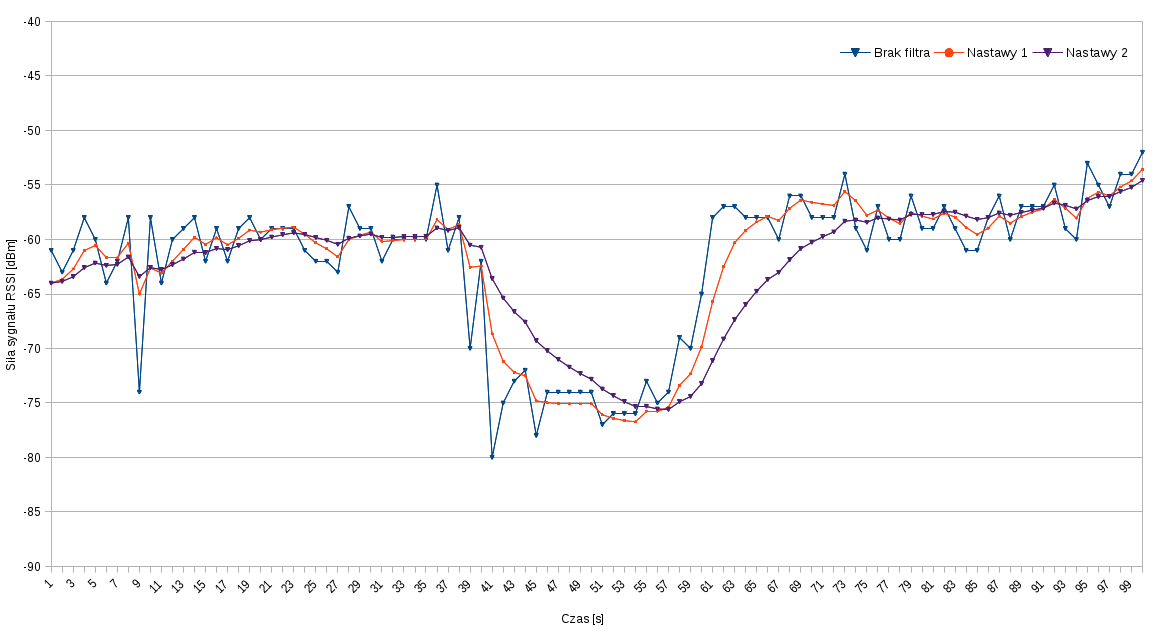
\includegraphics[width=0.9\textwidth]{img/filtr-propab.png}
\caption{Filtr probabilistyczny}
\label{fig:filtry-probab}
\end{figure}
Na wykresie \ref{fig:filtry-wszystkie} przedstawiono przebieg RSSI bez filtracji, z filtracją średnią ruchomą dla $N=5$ oraz filtracją probabilistyczną wg. nastaw 1. Filtr średniej ruchomej ma znacznie większą bezwładność od filtra probabilistycznego. Dlatego do testowania lokalizacji robota wykorzystano właśnie filtr probabilistyczny, jako lepiej radzący sobie w sytuacjach dynamiczych. 
\begin{figure}[H]
\centering
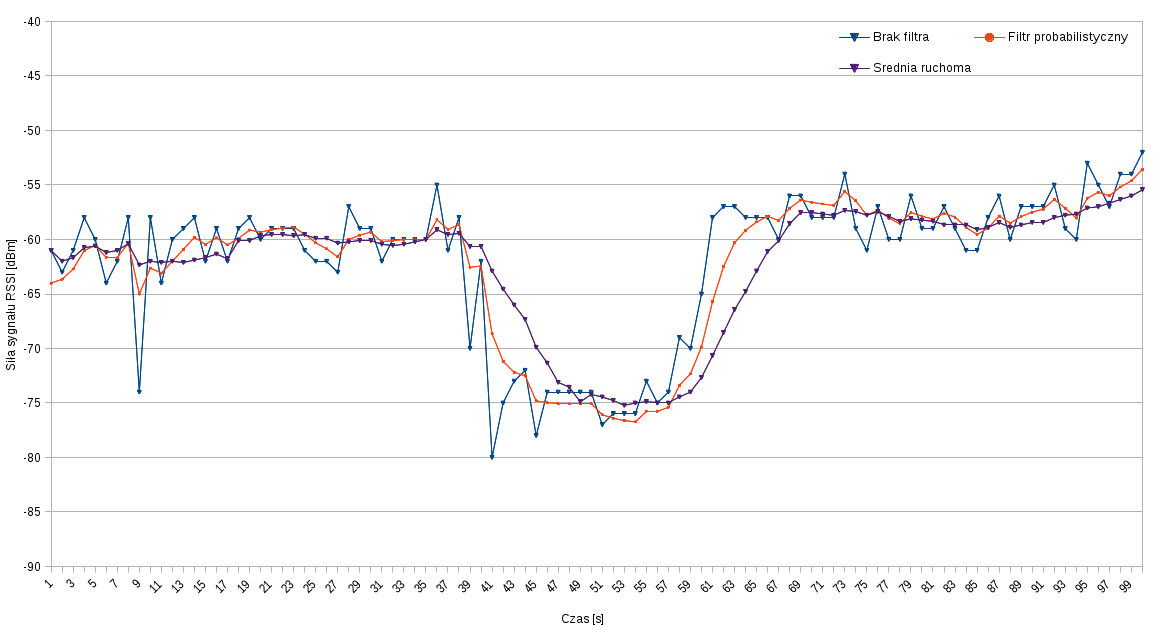
\includegraphics[width=0.9\textwidth]{img/filtry-porownanie.png}
\caption{Porównanie metod filtracji}
\label{fig:filtry-wszystkie}
\end{figure}

\section{Porównanie metod lokalizacji}
W niniejszej sekcji opisano przebieg i wyniki badania zasadniczej części niniejszej pracy - algorytmu lokalizacji. W celu wykonania badań, konieczne było zbudowanie mapy środowiska pracy robota oraz skalibrowanie znaczników, tj. wyznaczenie parametrów modelu \ref{eq:logfit_d}. 
\subsection{Metodyka badań}
Badania metod lokalizacji przeprowadzono na opisanym w rozdziale \ref{sec:hardware} robocie Pioneer 3-AT, w pomieszczeniu Laboratorium Robotyki Mobilnej Wydziału Mechatroniki PW. Do zbudowania mapy pomieszczenia, potrzebnej do pomiarów, wykorzystano program Gmapping. Budowanie mapy polegało na wykonaniu 3 przejazdów dookoła pomieszczenia. W trakcie przejazdów unikano gwałtownych przyspieszeń, hamowań i skrętów robota, w celu ograniczenia uślizgu kół, który wprowadza błąd do mapowania SLAM. 
Tak wyznaczoną mapę zapisano w pliku graficznym PNG. Jeden piksel obrazka reprezentował 5 cm przestrzeni. Następnie zlokalizowano na mapie umiejscowienie znaczników, korzystając z punktów charakterystycznych. 

W celu skalibrowania znaczników zebrano szereg punktów pomiarowych w różnych odległościach od znacznika. Aby wyeliminować wpływ wahań RSSI na wyznaczony model, każdy pomiar składał się z 20 uśrednionionych wartości RSSI.  Następnie wyznaczono model w oparciu o interpolację i dopasowanie funkcji wykładniczej. 

Do badania metod lokalizacji jako odniesienie wykorzystano lokalizację AMCL. Po wykonaniu kilku przejazdów robota po pomieszczeniu oparta o filtr cząsteczkowy lokalizacja AMCL zapewnia dokładność zbliżoną do rozdzielczości mapy, co najmniej o rząd wielkości lepszą niż dokładność lokalizacji w oparciu o znaczniki. Aby zapewnić rzetelne porównanie metod lokalizacji, posłużono się danymi nagranymi programem Rosbag, zatem obydwie metody zostały użyte na identycznych danych testowych. 

W obydwu metodach porównano wyniki lokalizacji obliczone z odległości przefiltrowanych przez poszczególne filtry (por. \ref{sec:testy-filtracja}).
\subsection{Wyniki}

\subsubsection{Mapa środowiska}
Rysunek \ref{fig:mapa} przedstawia wyznaczoną metodą SLAM mapę laboratorium. Punkty w kolorze szarym oznaczają obszar wolny, zaś w kolorze czarnym - zajęty. Pojedyncze czarne punkty i szare linie stanowią wynik zakłóceń SLAM i nie mają negatywnego wpływu na lokalizację. Obszar w prawym dolnym rogu mapy obrazuje otwarte drzwi do sąsiedniego pomieszczenia, które nie było objęte mapowaniem. Na mapie zobrazowane są pozycje początków układów współrzędnych: mapy oraz 3 znaczników. 
\begin{figure}[H]
\centering
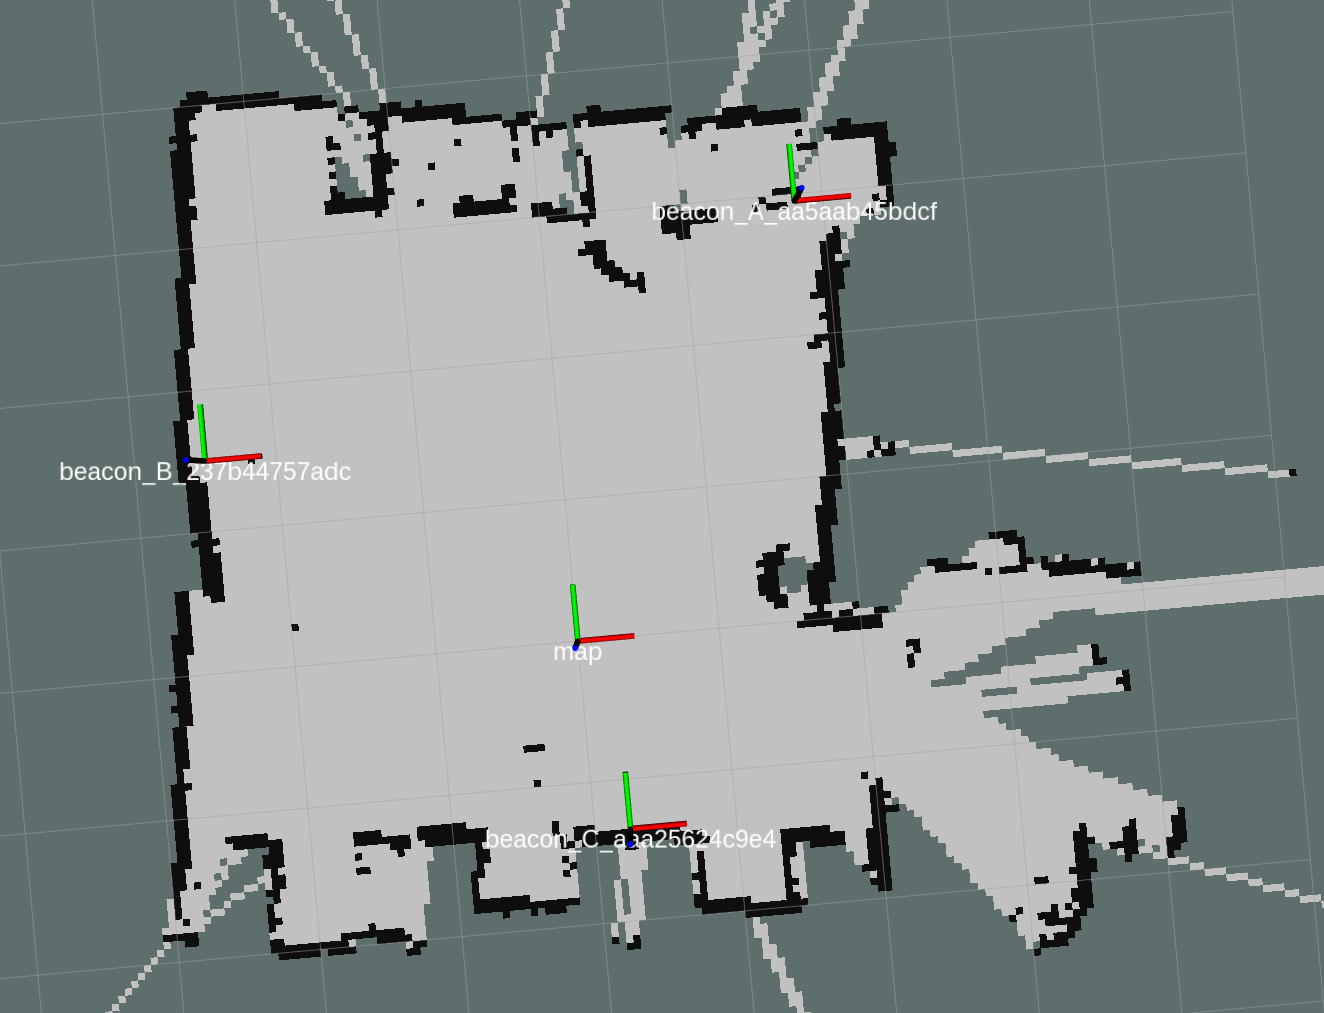
\includegraphics[width=0.9\textwidth]{img/mapa2.png}
\caption{Mapa środowiska wyznaczona metodą SLAM za pomocą programu GMapping z zaznaczonymi znacznikami radiowymi.}
\label{fig:mapa}
\end{figure}


\subsubsection{Kalibracja znaczników}

Tabela \ref{tab:strojenie} przedstawia wyniki kalibracji znaczników. Z wyników pomiaru usunięto punkty znacząco odbiegające od oczekiwanego przebiegu. Dopasowane krzywe wraz z punktami pomiarowymi wykreślono na rys. \ref{fig:strojenie-a}, \ref{fig:strojenie-b} oraz \ref{fig:strojenie-c}.

\begin{table}[H]
 \caption{Wyniki kalibracji}
 \label{tab:strojenie}
 \begin{tabular}{|l|l|l|}
  \hline
  \textbf{Znacznik}	& \textbf{Interpolacja} & \textbf{Dopasowanie krzywej potęgowej }\\ \hline
  A 		& $a=50,515$, $b=28,631$	& $a=50,167$, $b=28,480$	\\ \hline
  B 		& $a=65,036$, $b=11,547$	& $a=66,028$, $b=10,074$	\\ \hline
  C 		& $a=65,468$, $b=7,319$		& $a=68,215$, $b=0,984$		\\ \hline
 \end{tabular}

\end{table}


\begin{figure}[H]
\centering
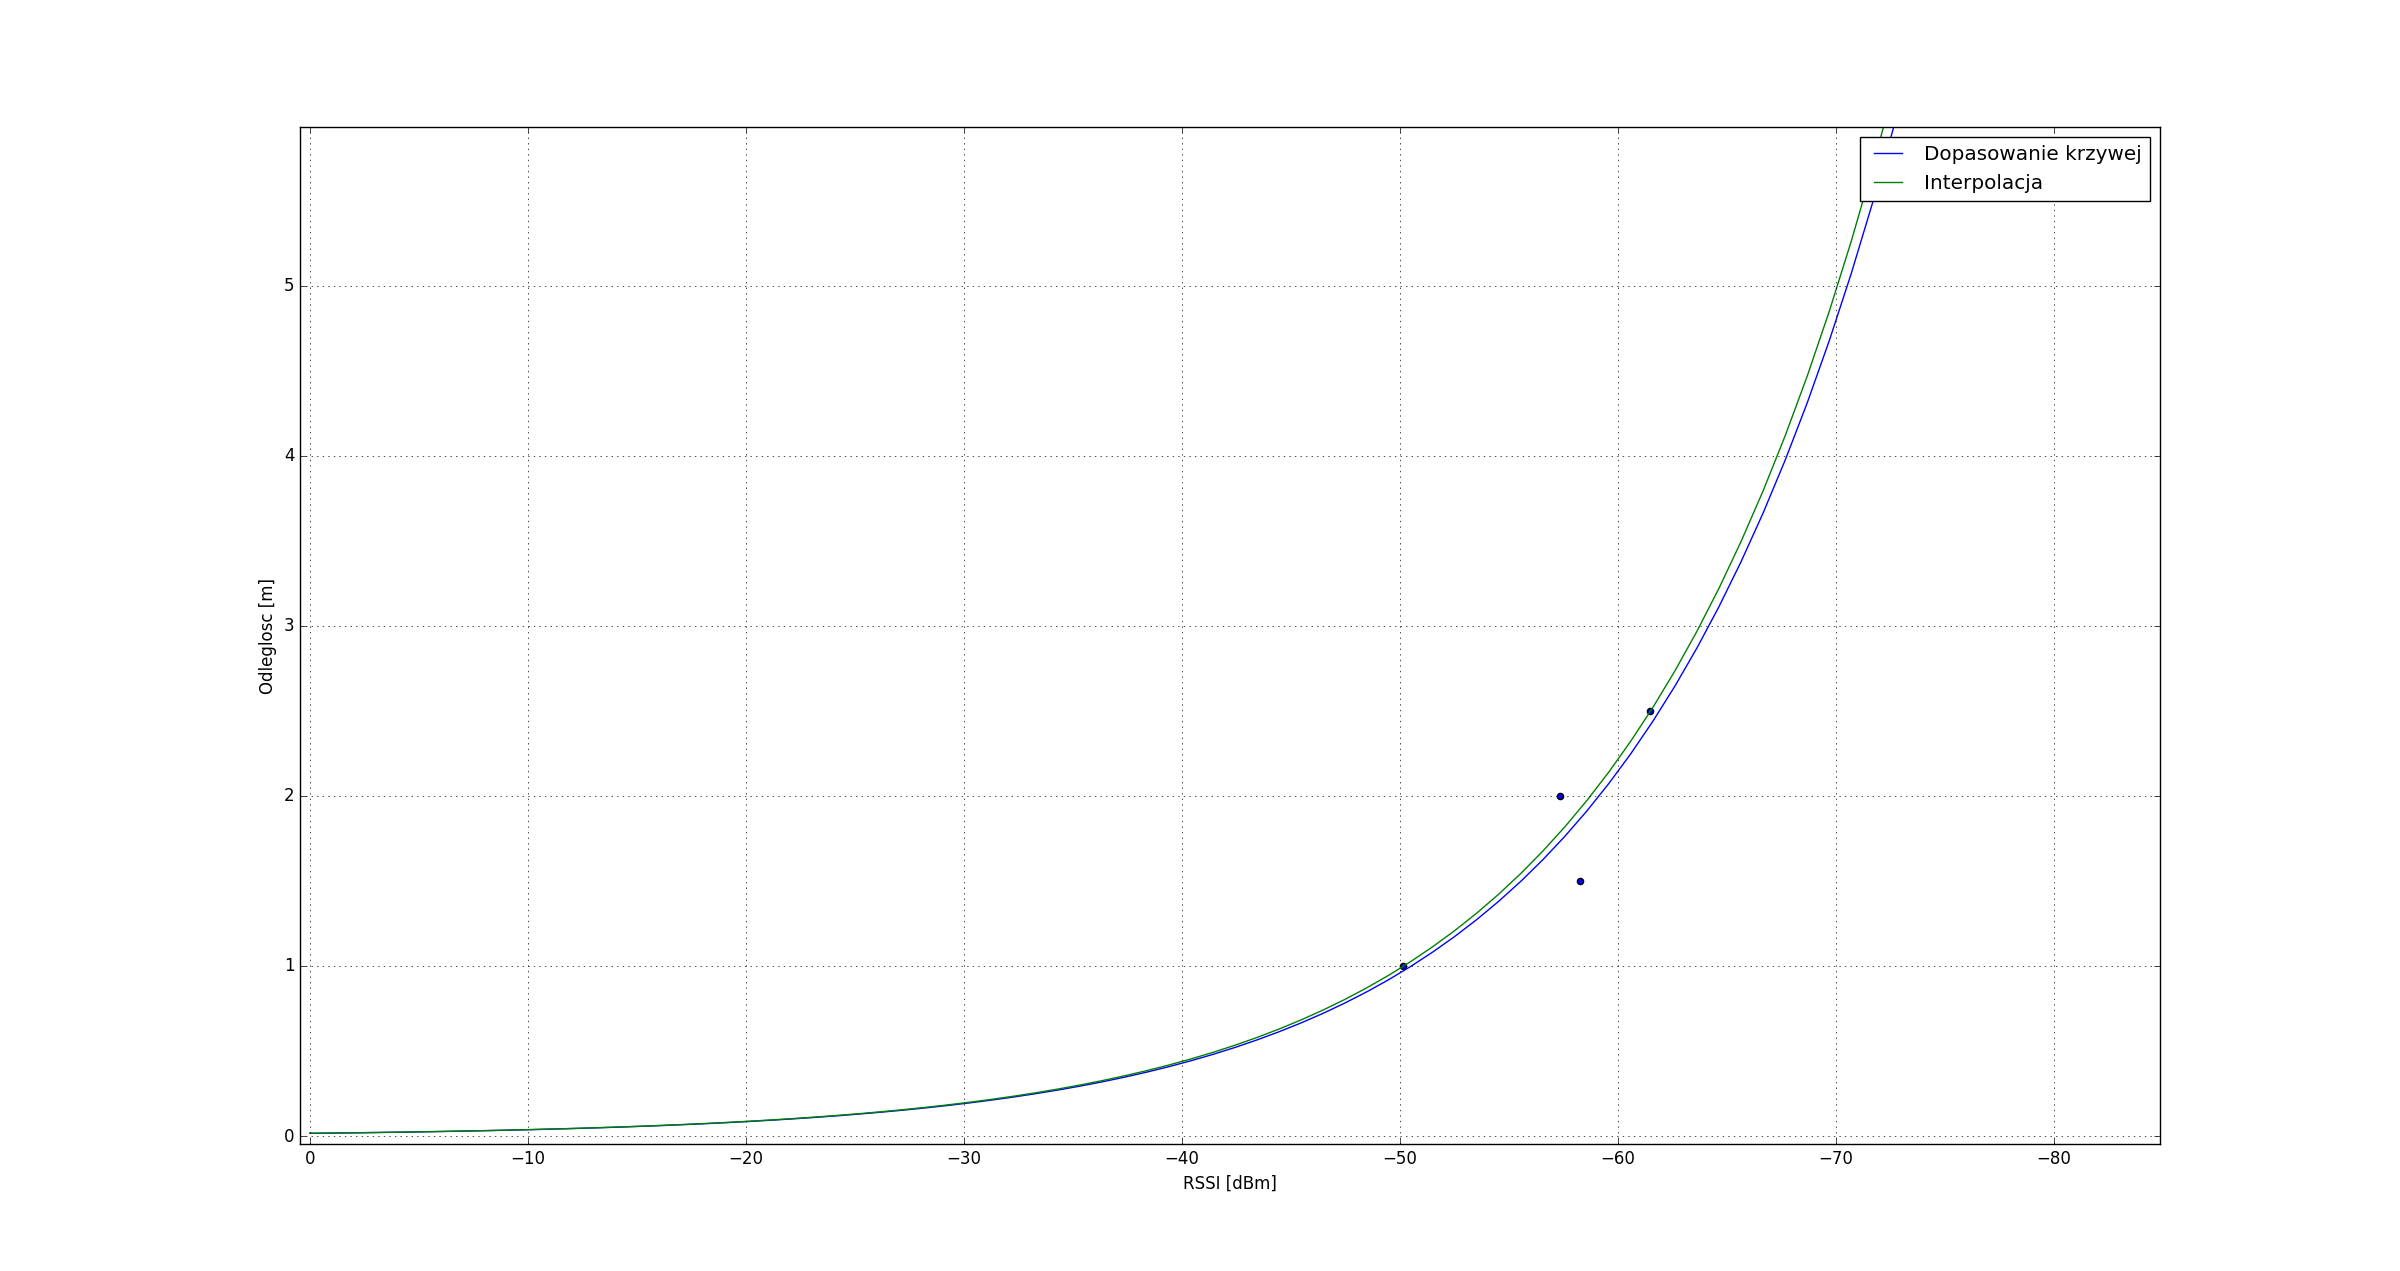
\includegraphics[width=1\textwidth]{img/strojenie-a.png}
\caption{Wyznaczanie modelu znacznika A}
\label{fig:strojenie-a}
\end{figure}

\begin{figure}[H]
\centering
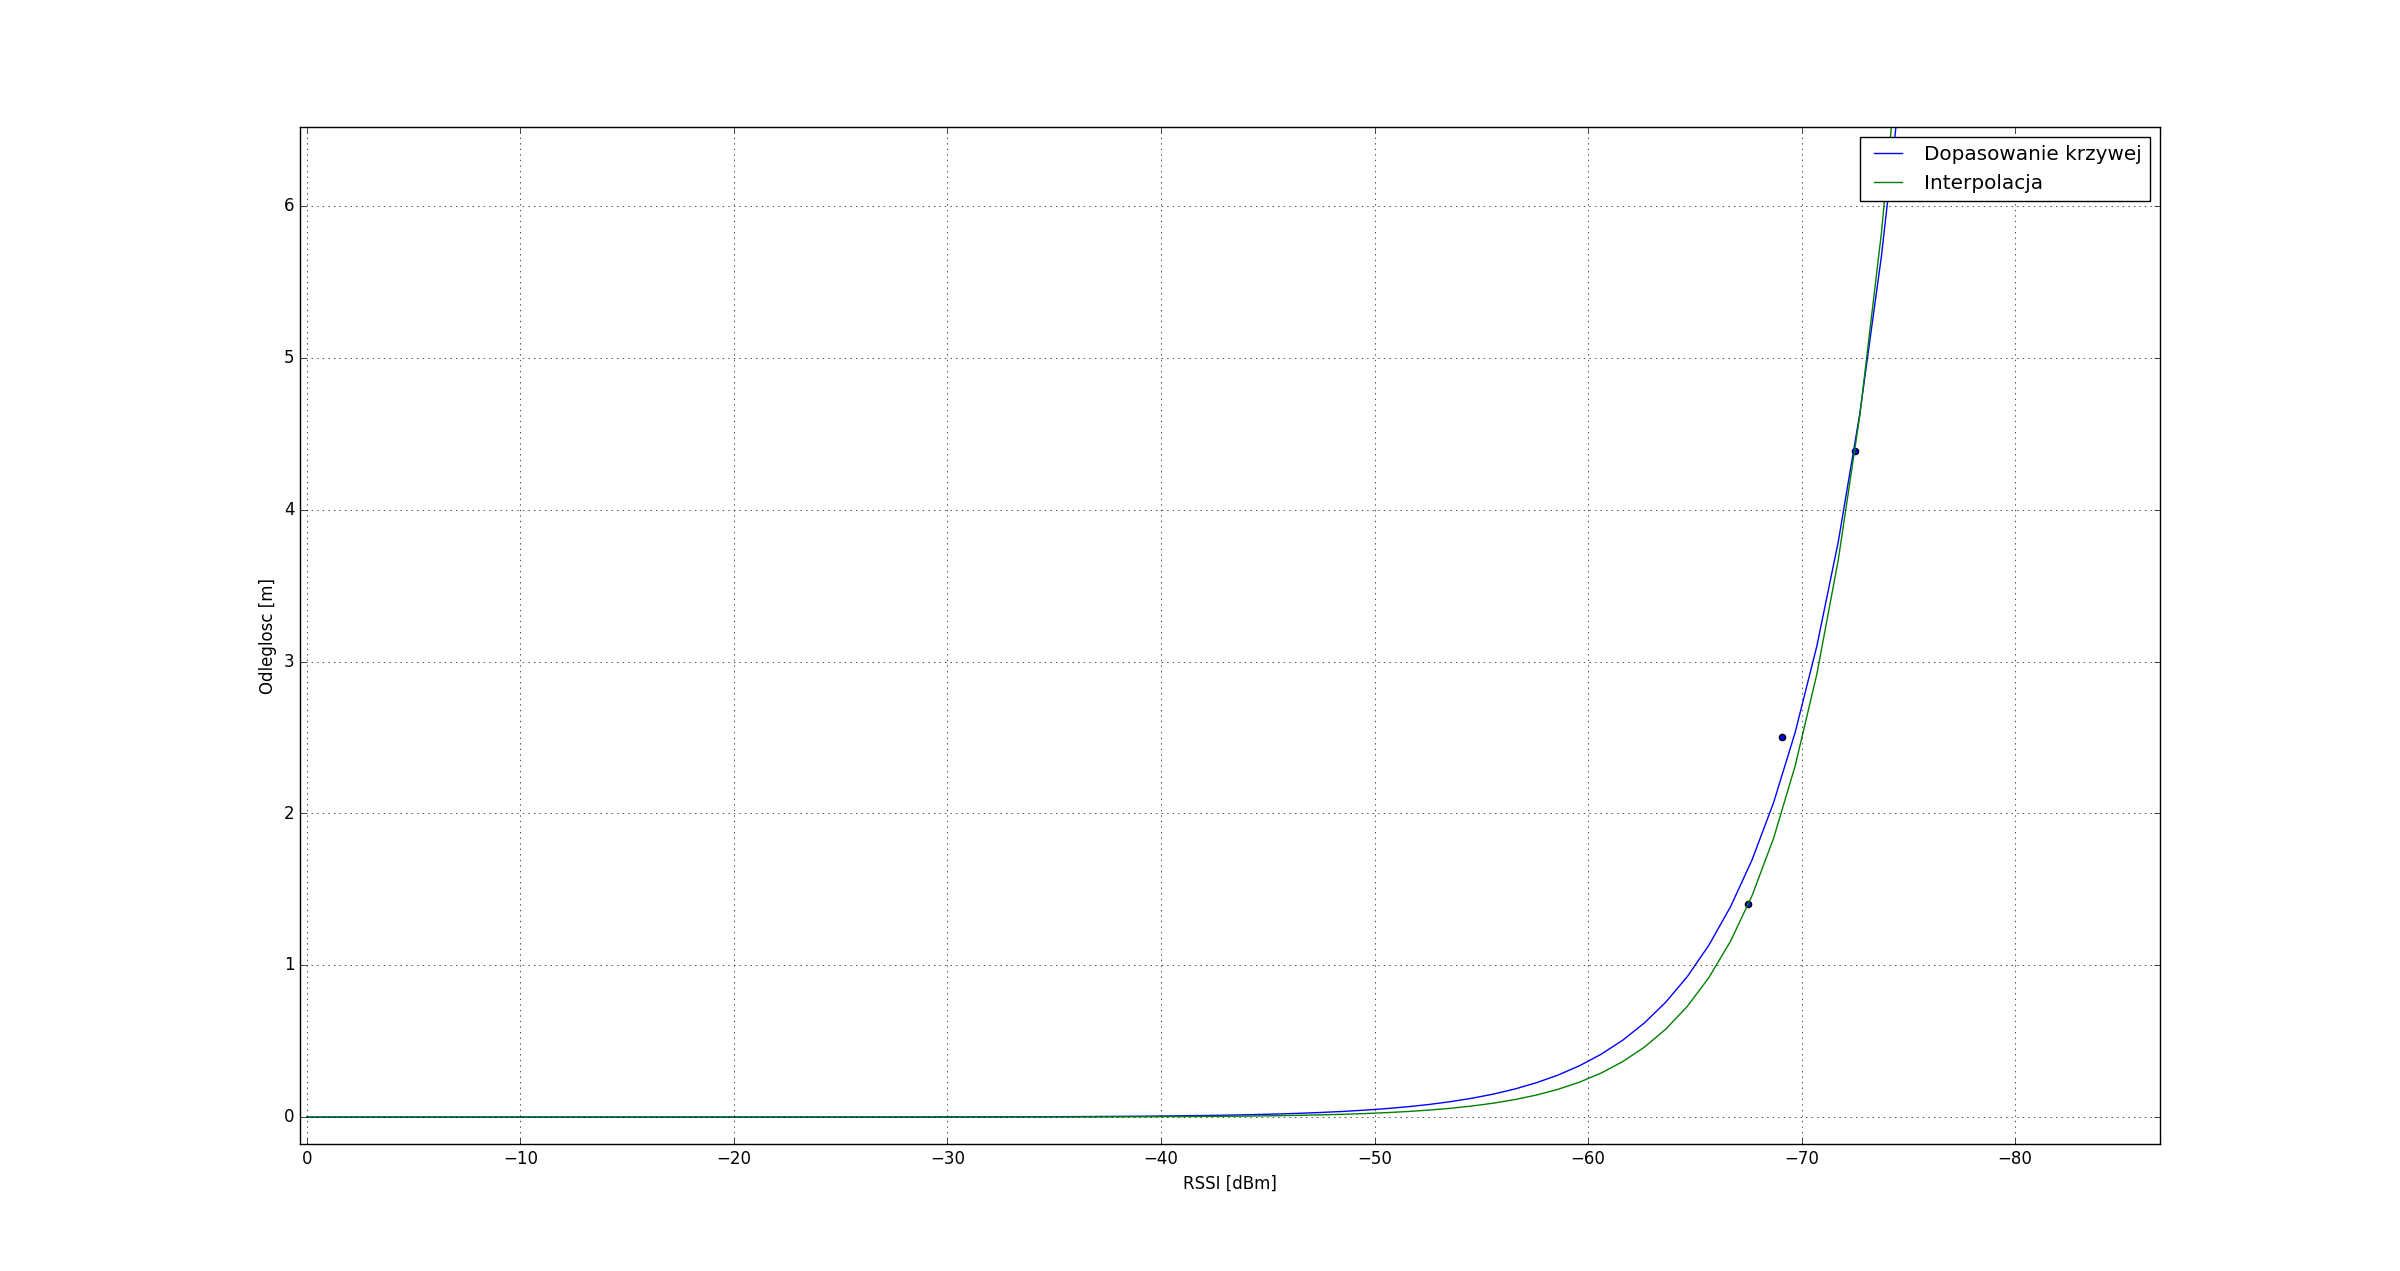
\includegraphics[width=1\textwidth]{img/strojenie-b.png}
\caption{Wyznaczanie modelu znacznika B}
\label{fig:strojenie-b}
\end{figure}

\begin{figure}[H]
\centering
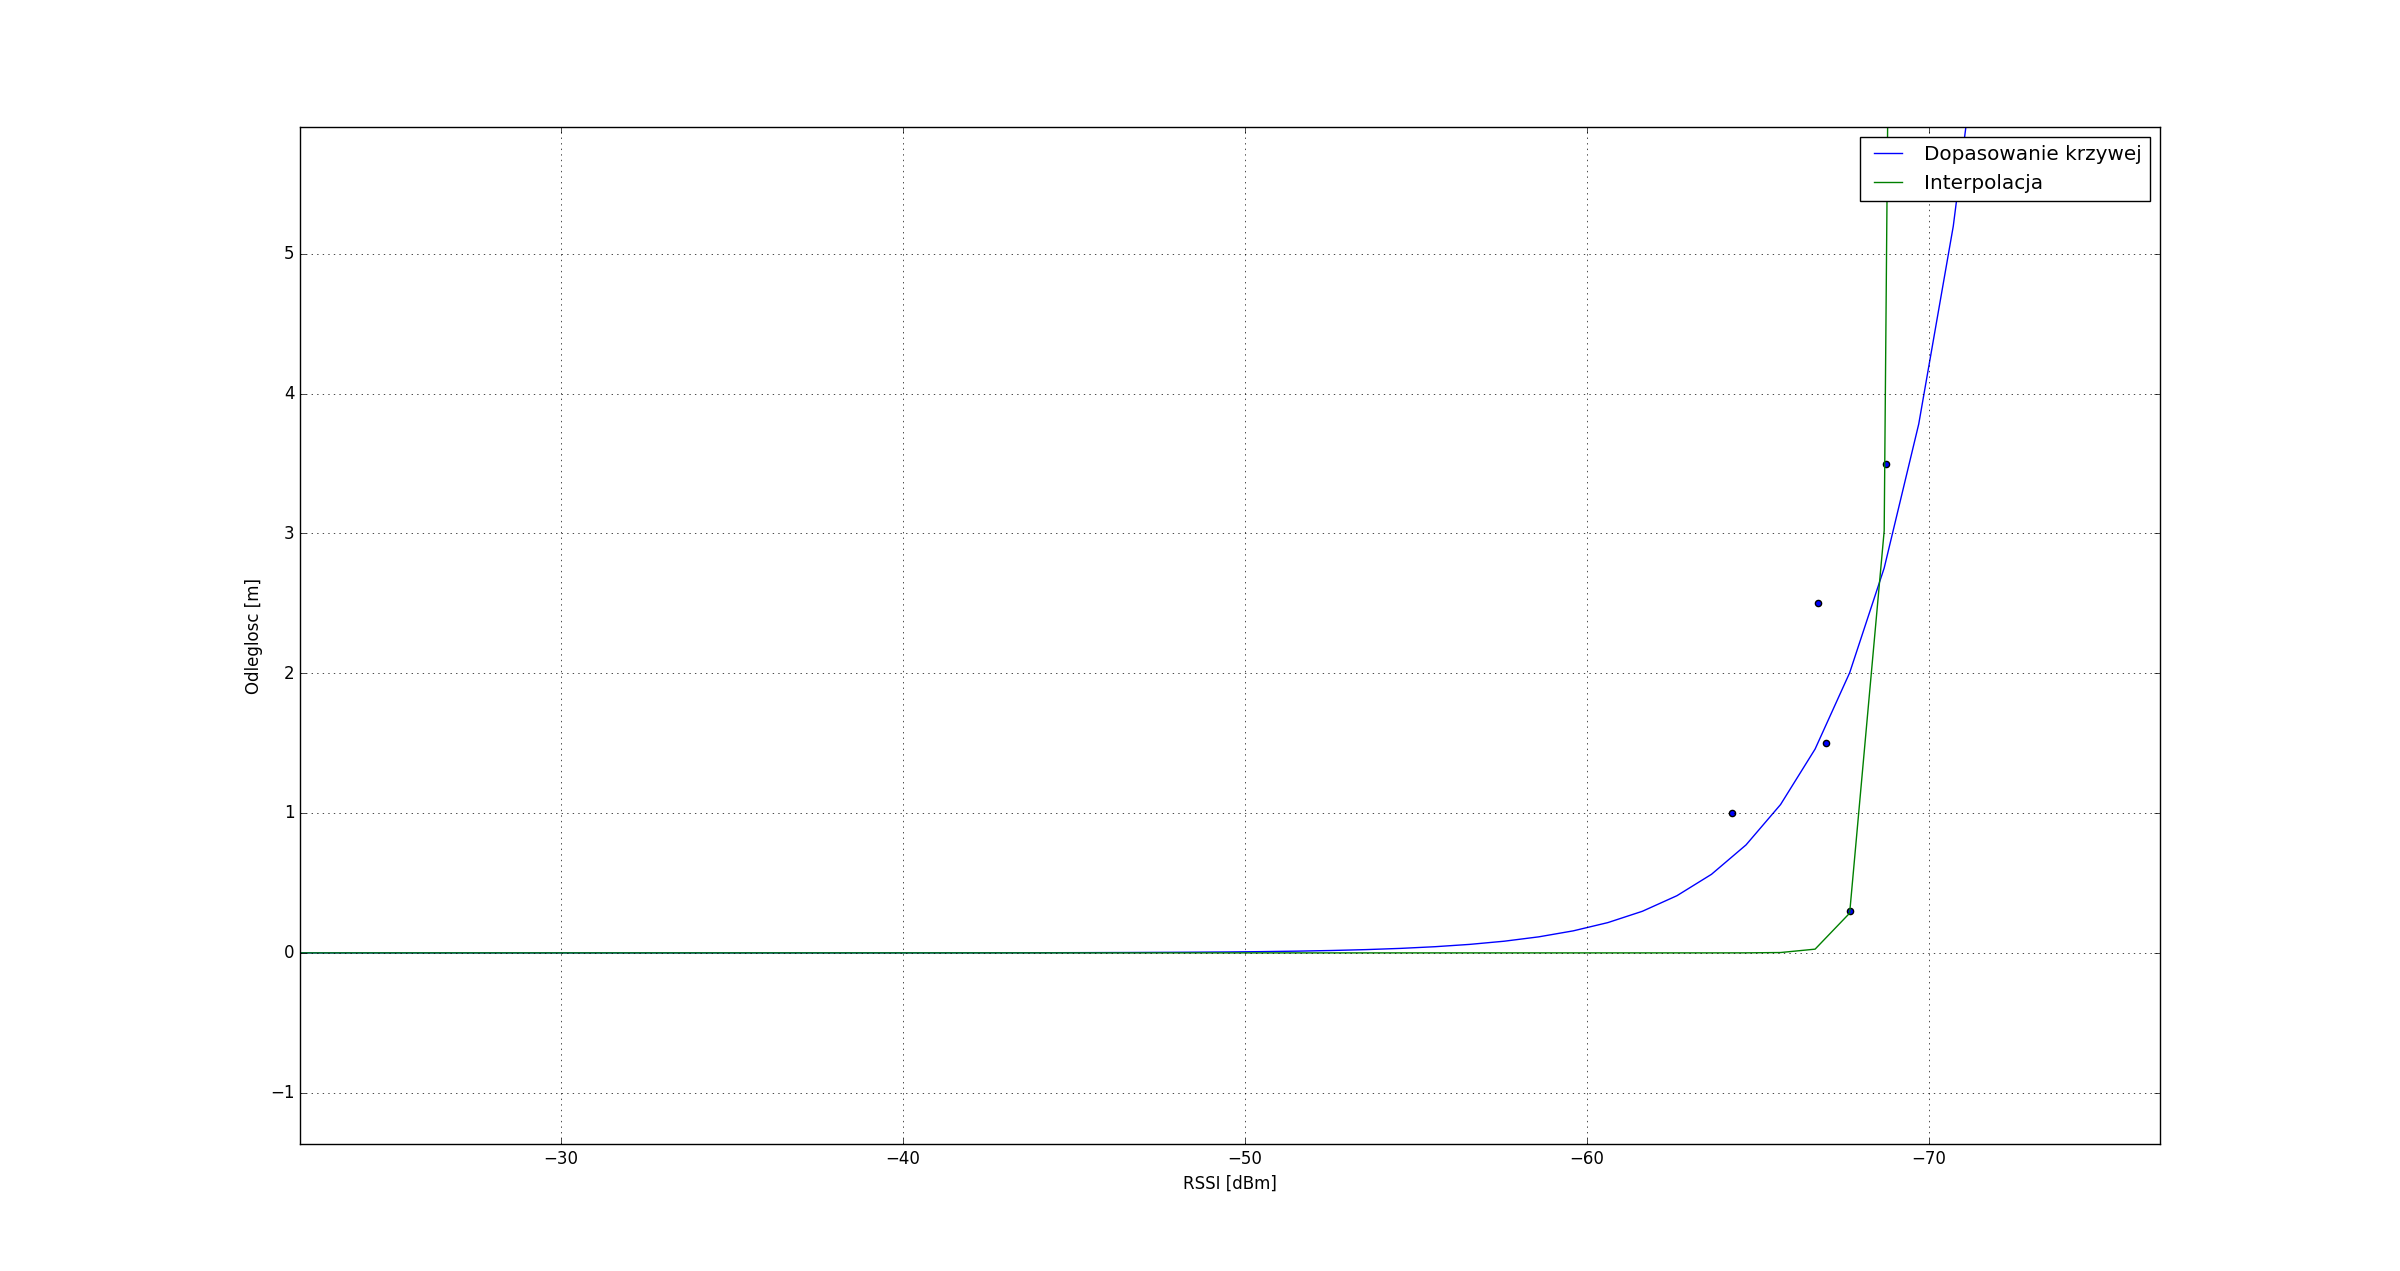
\includegraphics[width=1\textwidth]{img/strojenie-c.png}
\caption{Wyznaczanie modelu znacznika C}
\label{fig:strojenie-c}
\end{figure}

\subsubsection{Trilateracja}
Pierwsze próby lokalizacji za pomocą trilateracji przeprowadzono wykorzystując model wyznaczony w poprzednim punkcie metodą dopasowania krzywej. Jednakże, jak pokazuje rys. \ref{fig:trilat-przegryw}, nastawy te powodują bardzo duży rozrzut wyników pomiaru - większość wyznaczonych położeń robota wypada poza mapą i nie ma związku z rzeczywistym jego położeniem. Rys. \ref{fig:trilat-przegryw} obrazuje ten problem dla jednego punktu pomiarowego, jednakże podobnie duży rozrzut występuje również dla pozostałych punktów. Należy zwrócić uwagę na inną skalę osi wykresu \ref{fig:trilat-przegryw} w porównaniu do wykresów  \ref{fig:trilat-first} - \ref{fig:trilat-last}. Dyskusję możliwych przyczyn takiego zachowania przedstawiono w rozdziale \ref{ch:wnioski}.

Dlatego też podjęto próbę wyznaczenia właściwego modelu ręcznie, metodą prób i błędów. Bazując na modelach wyznacznonych automatycznie, wykorzystując narzędzie Rosbag oraz narzędzia do wykreślania zależności siły sygnału od odległości, dobrano model zapewniający wyniki o mniejszym rozrzucie:
\begin{equation}
 a=50, b=50
\end{equation}

Wyniki z wykorzystaniem modelu wyznaczonego ręcznie pokazują rys. \ref{fig:trilat-first} - \ref{fig:trilat-last}. Dla porównania, rysunki te, z wyjątkiem rys. \ref{fig:trilat-przegryw} posiadają jednakową skalę. Rysunek \ref{fig:trilat-przegryw} ma zmienioną skalę aby ukazać problem rozrzutu wyników. 

Na rysunkach, czerwony krzyżyk oznacza punkt odniesienia, niebieskie kropki symbolizują wyniki trilateracji. Na rysunku \ref{fig:referencyjne} przedstawiono położenie kolejnych punktów odniesienia.
\begin{figure}[H]
\centering
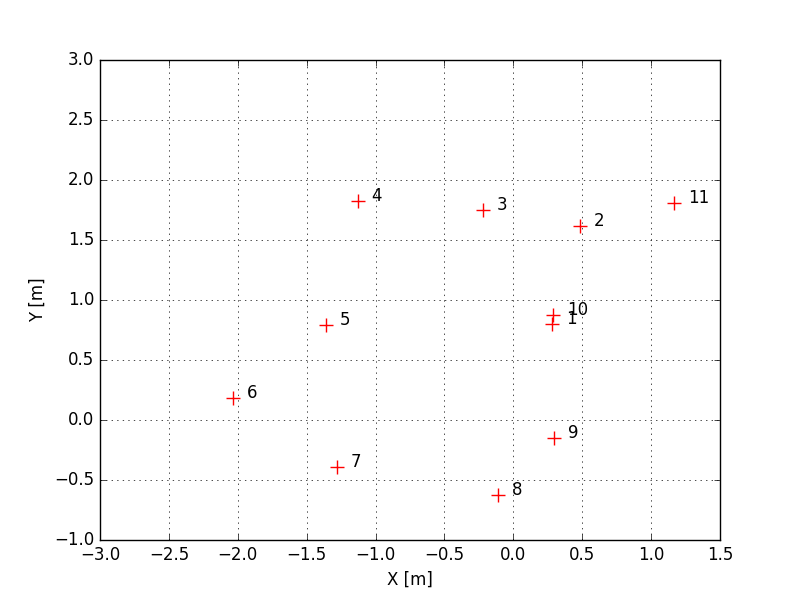
\includegraphics[width=0.7\textwidth]{img/references.png}
\caption{Położenie punktów pomiarowych.}
\label{fig:referencyjne}
\end{figure}
\begin{figure}[H]
\centering
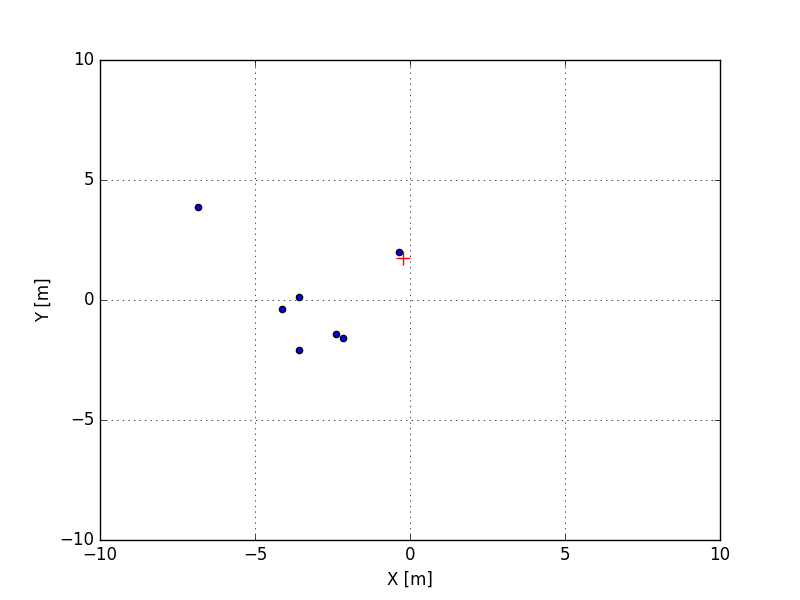
\includegraphics[width=0.7\textwidth]{img/trilat-przegryw.png}
\caption{Wyniki trilateracji dla modelu obliczonego przez dopasowanie krzywej}
\label{fig:trilat-przegryw}
\end{figure}
\begin{figure}[H]
\centering
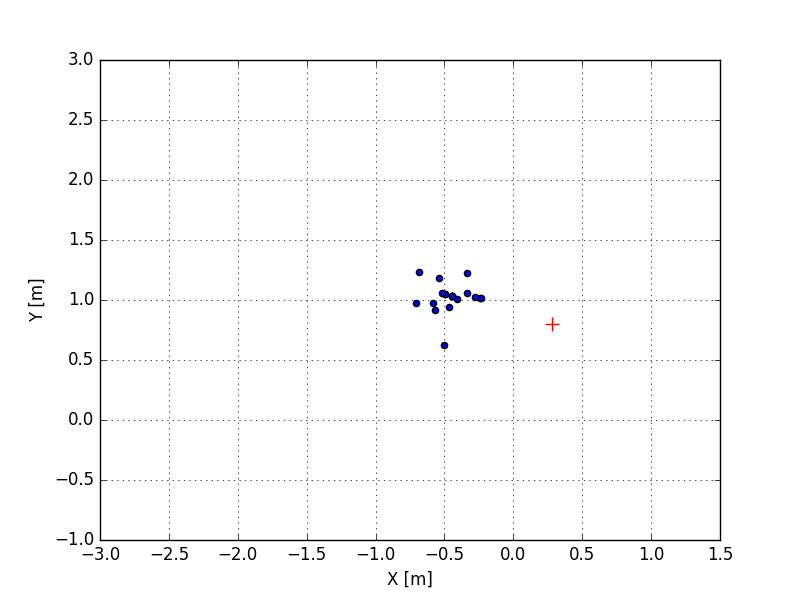
\includegraphics[width=0.7\textwidth]{img/trilat-map3-1.png}
\caption{Wyniki trilateracji dla ręcznie dobranego modelu - punkt 1}
\label{fig:trilat-first}
\end{figure}
\begin{figure}[H]
\centering
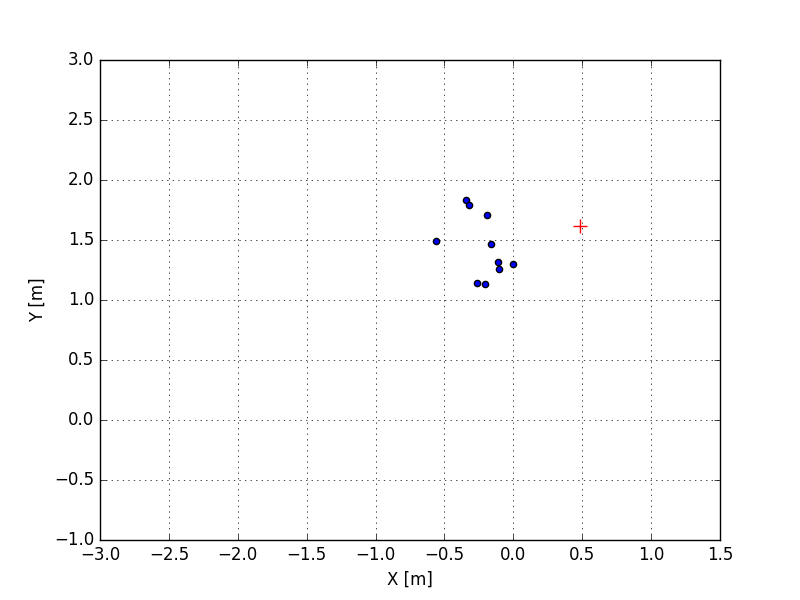
\includegraphics[width=0.7\textwidth]{img/trilat-map3-2.png}
\caption{Wyniki trilateracji dla ręcznie dobranego modelu - punkt 2}
\end{figure}
\begin{figure}[H]
\centering
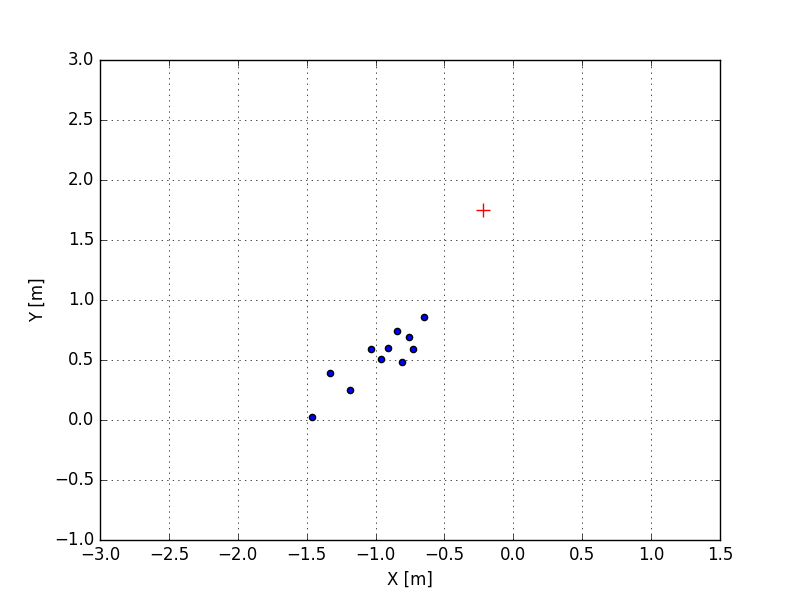
\includegraphics[width=0.7\textwidth]{img/trilat-map3-3.png}
\caption{Wyniki trilateracji dla ręcznie dobranego modelu - punkt 3}
\end{figure}
\begin{figure}[H]
\centering
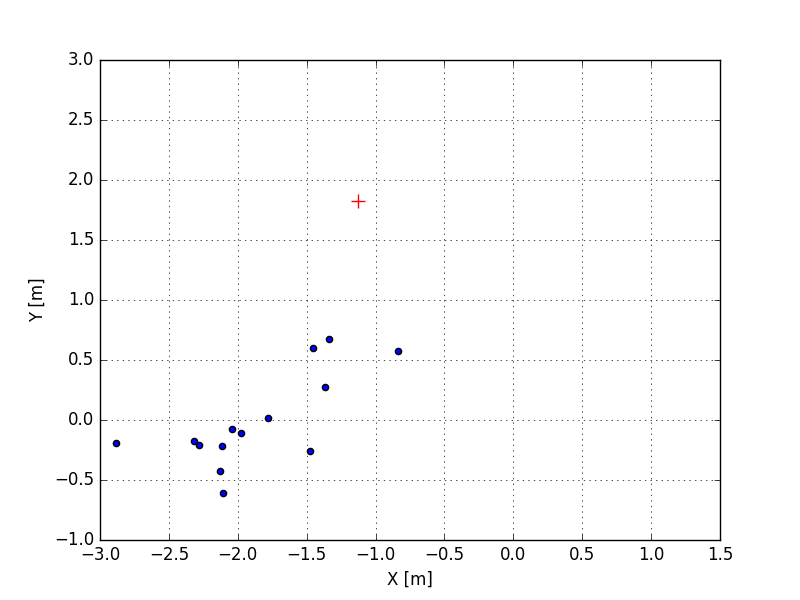
\includegraphics[width=0.7\textwidth]{img/trilat-map3-4.png}
\caption{Wyniki trilateracji dla ręcznie dobranego modelu - punkt 4}
\end{figure}
\begin{figure}[H]
\centering
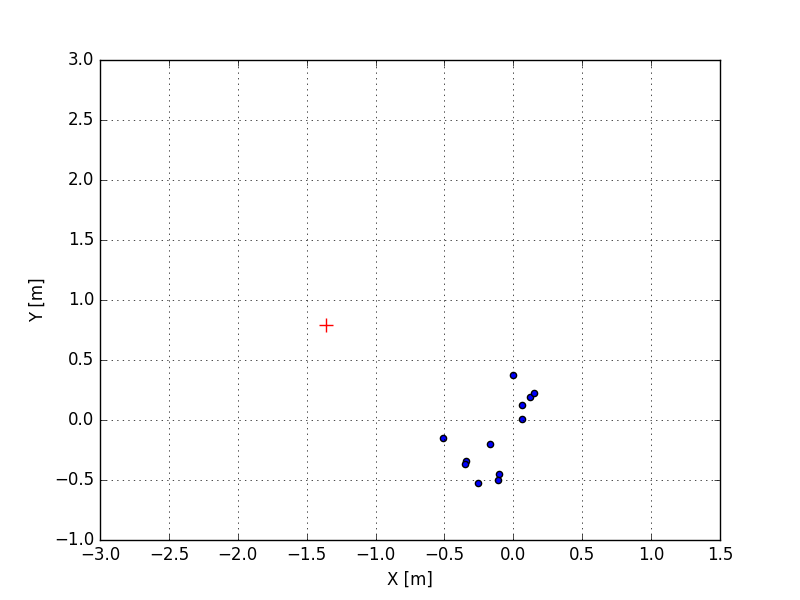
\includegraphics[width=0.7\textwidth]{img/trilat-map3-5.png}
\caption{Wyniki trilateracji dla ręcznie dobranego modelu - punkt 5}
\end{figure}
\begin{figure}[H]
\centering
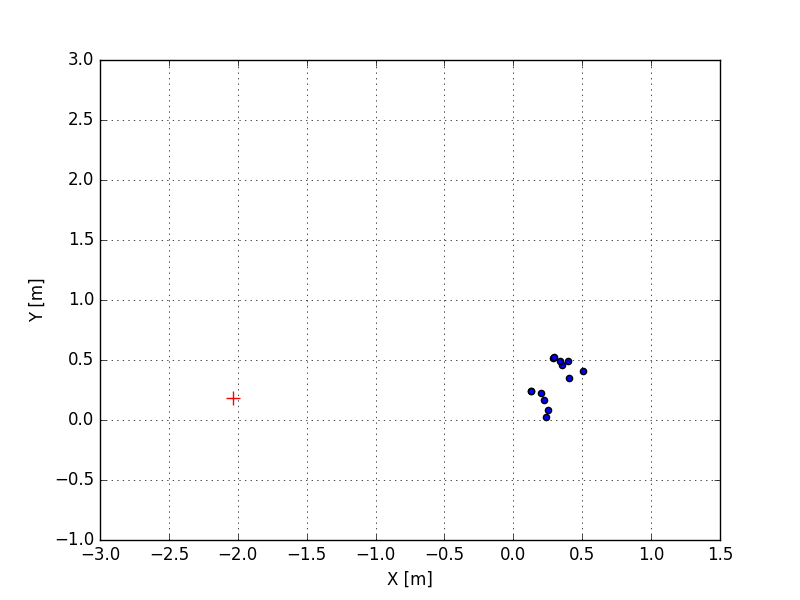
\includegraphics[width=0.7\textwidth]{img/trilat-map3-6.png}
\caption{Wyniki trilateracji dla ręcznie dobranego modelu - punkt 6}
\end{figure}
\begin{figure}[H]
\centering
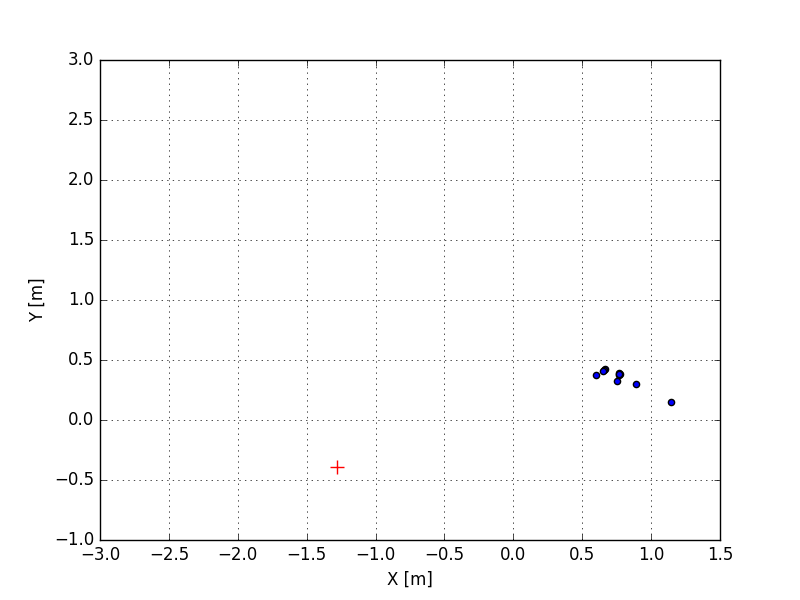
\includegraphics[width=0.7\textwidth]{img/trilat-map3-7.png}
\caption{Wyniki trilateracji dla ręcznie dobranego modelu - punkt 7}
\end{figure}
\begin{figure}[H]
\centering
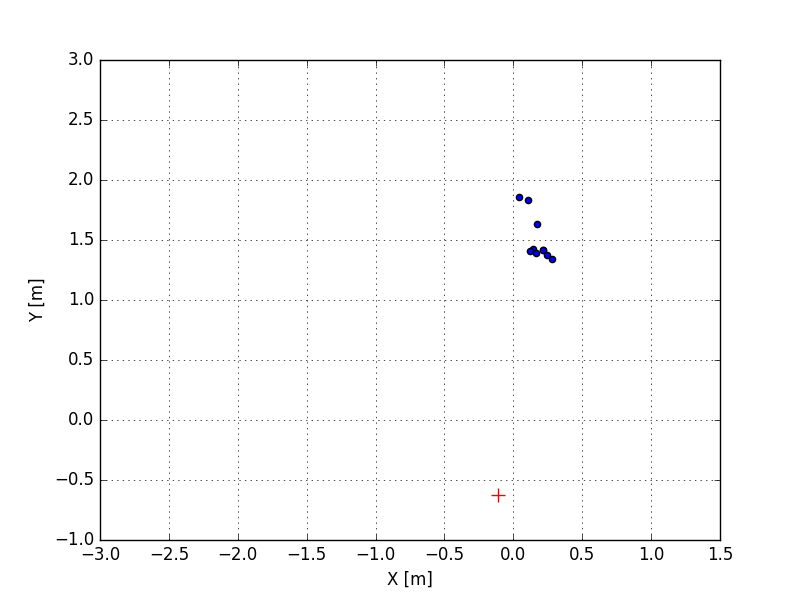
\includegraphics[width=0.7\textwidth]{img/trilat-map3-8.png}
\caption{Wyniki trilateracji dla ręcznie dobranego modelu - punkt 8}
\end{figure}
\begin{figure}[H]
\centering
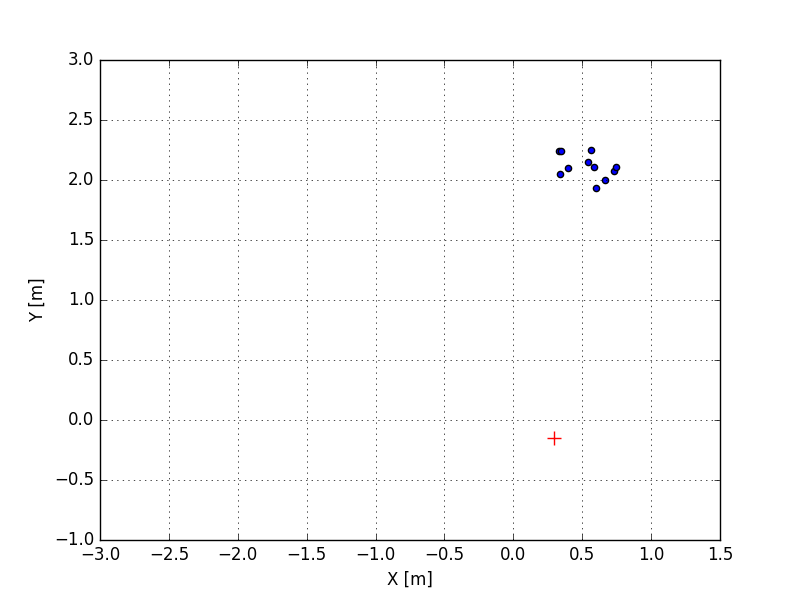
\includegraphics[width=0.7\textwidth]{img/trilat-map3-9.png}
\caption{Wyniki trilateracji dla ręcznie dobranego modelu - punkt 9}
\end{figure}
\begin{figure}[H]
\centering
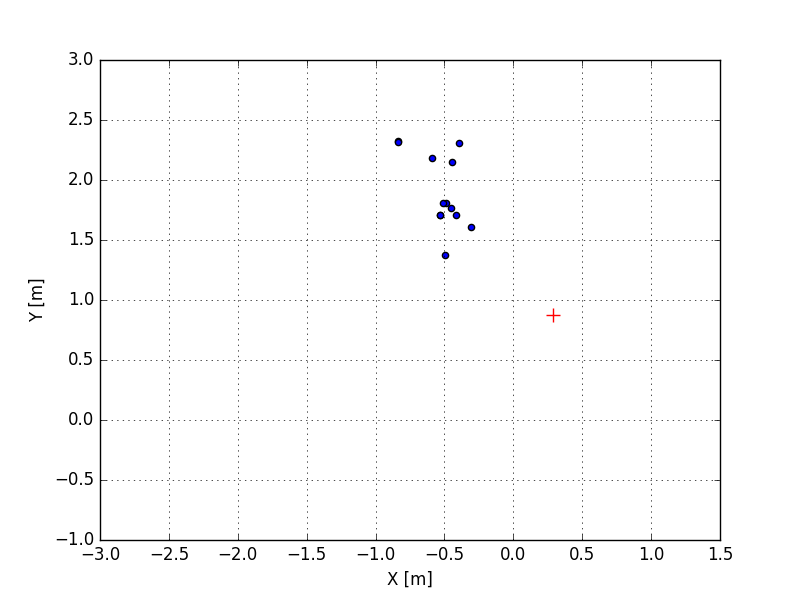
\includegraphics[width=0.7\textwidth]{img/trilat-map3-10.png}
\caption{Wyniki trilateracji dla ręcznie dobranego modelu - punkt 10}
\end{figure}
\begin{figure}[H]
\centering
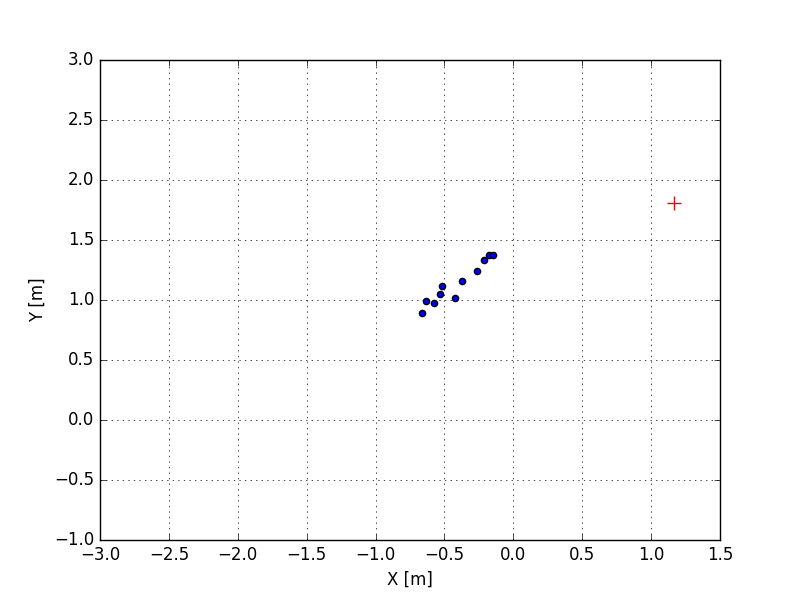
\includegraphics[width=0.7\textwidth]{img/trilat-map3-11.png}
\caption{Wyniki trilateracji dla ręcznie dobranego modelu - punkt 11}
\label{fig:trilat-last}
\end{figure}


\subsubsection{Filtr cząsteczkowy}
Jak wspomniano wcześniej, badanie filtra cząsteczkowego przeprowadzono na tym samym zbiorze danych co badania metody trilateracji. Podobnie jak w wypadku trilateracji, wykorzystano model wyznacznony ręcznie. Wyniki lokalizacji w poszczególnych punktach ukazują wykresy \ref{fig:pf-first} - \ref{fig:pf-last}. Można zauważyć, że na wykresach zaznaczono miejszą ilość punktów wynikowych niż w wypadku trilateracji. Ta różnica wynika z faktu, że wynik trilateracji jest publikowany w stałym interwale (1 sekunda), natomiast filtr cząsteczkowy jest przeliczany tylko wtedy, kiedy odległość liniowa lub kątowa pokonana przez robota i zmierzona za pomocą odometrii przekroczy pewien próg. Jest to związane z optymalizacją wydajności programu. Dlatego też, kiedy robot jest nieruchomy, nowe punkty nie są publikowane - bowiem byłyby identyczne jak poprzednie.


\begin{figure}[H]
\centering
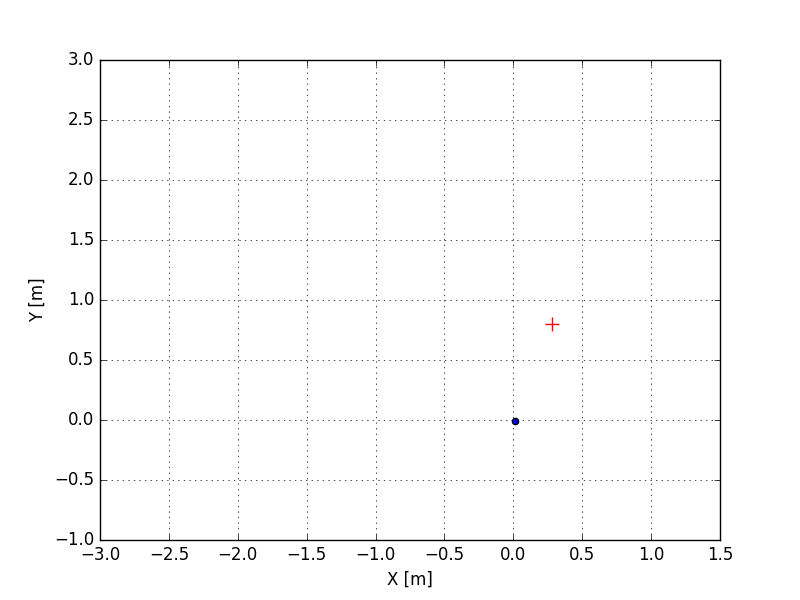
\includegraphics[width=0.7\textwidth]{img/pf-map3-1.png}
\caption{Wyniki lokalizacji za pomocą filtra cząsteczkowego dla ręcznie dobranego modelu - punkt 1}
\label{fig:pf-first}
\end{figure}
\begin{figure}[H]
\centering
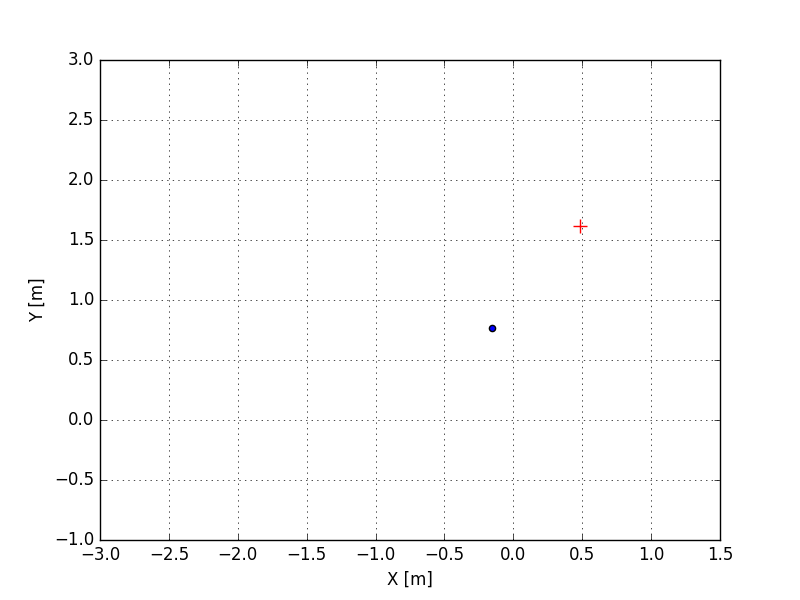
\includegraphics[width=0.7\textwidth]{img/pf-map3-2.png}
\caption{Wyniki lokalizacji za pomocą filtra cząsteczkowego dla ręcznie dobranego modelu - punkt 2}
\end{figure}
\begin{figure}[H]
\centering
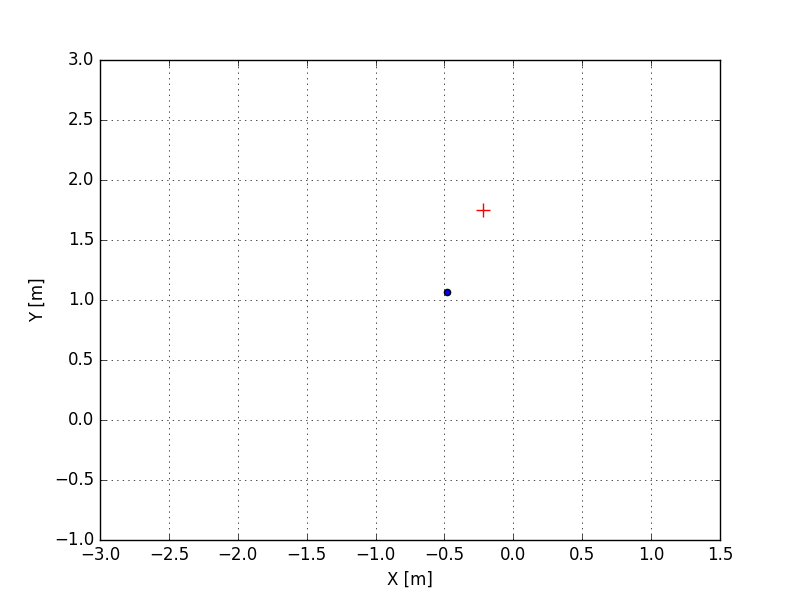
\includegraphics[width=0.7\textwidth]{img/pf-map3-3.png}
\caption{Wyniki lokalizacji za pomocą filtra cząsteczkowego dla ręcznie dobranego modelu - punkt 3}
\end{figure}
\begin{figure}[H]
\centering
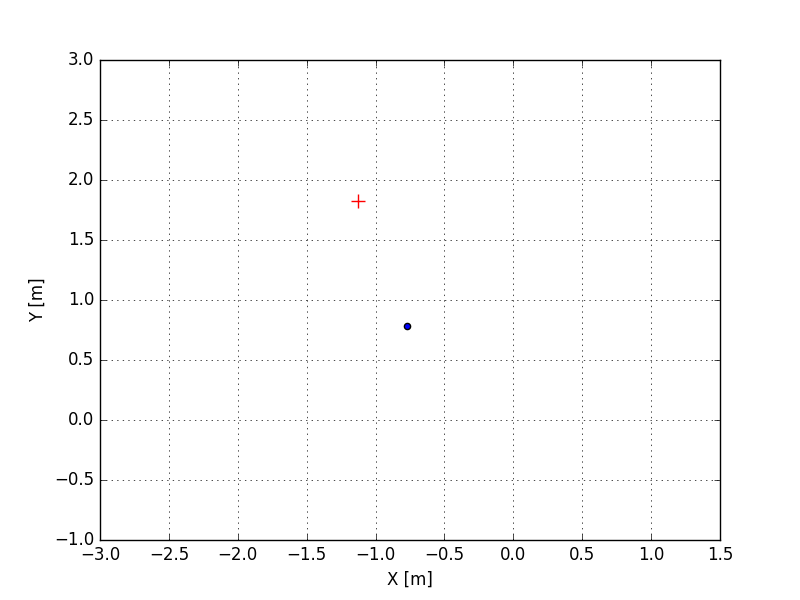
\includegraphics[width=0.7\textwidth]{img/pf-map3-4.png}
\caption{Wyniki lokalizacji za pomocą filtra cząsteczkowego dla ręcznie dobranego modelu - punkt 4}
\end{figure}
\begin{figure}[H]
\centering
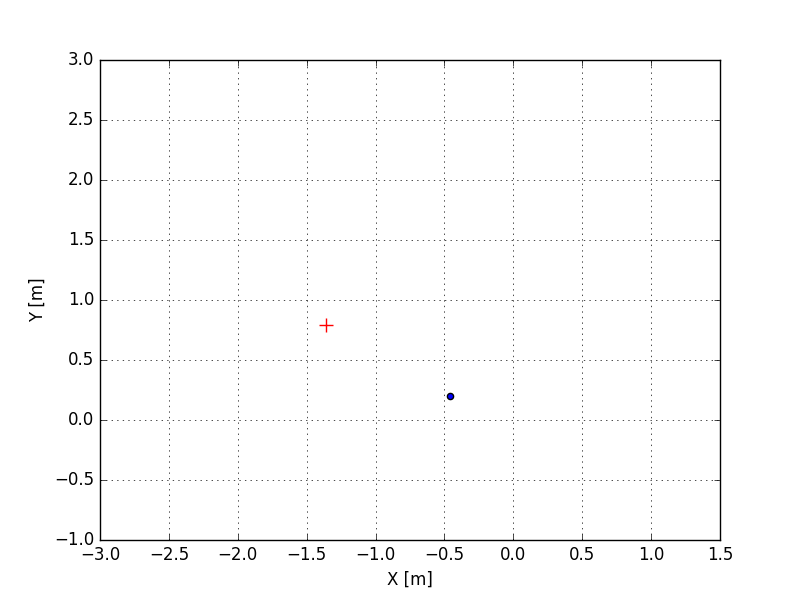
\includegraphics[width=0.7\textwidth]{img/pf-map3-5.png}
\caption{Wyniki lokalizacji za pomocą filtra cząsteczkowego dla ręcznie dobranego modelu - punkt 5}
\end{figure}
\begin{figure}[H]
\centering
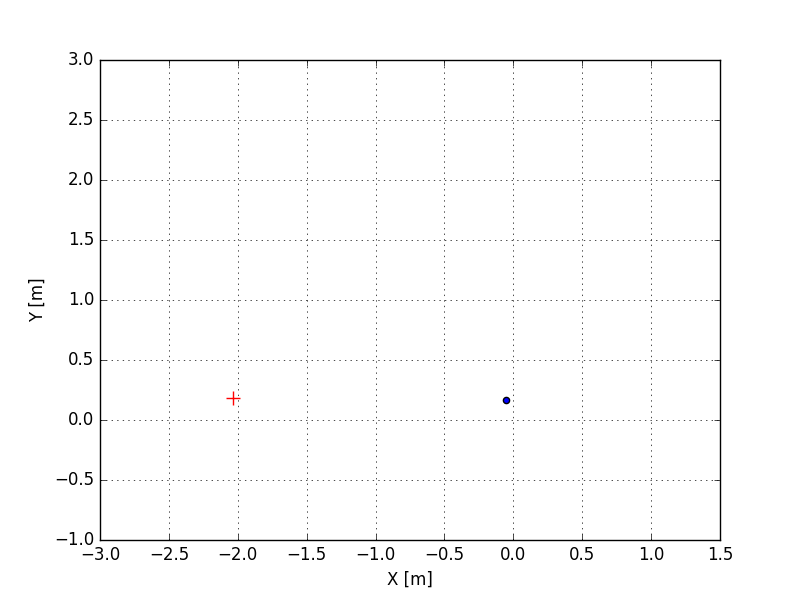
\includegraphics[width=0.7\textwidth]{img/pf-map3-6.png}
\caption{Wyniki lokalizacji za pomocą filtra cząsteczkowego dla ręcznie dobranego modelu - punkt 6}
\end{figure}
\begin{figure}[H]
\centering
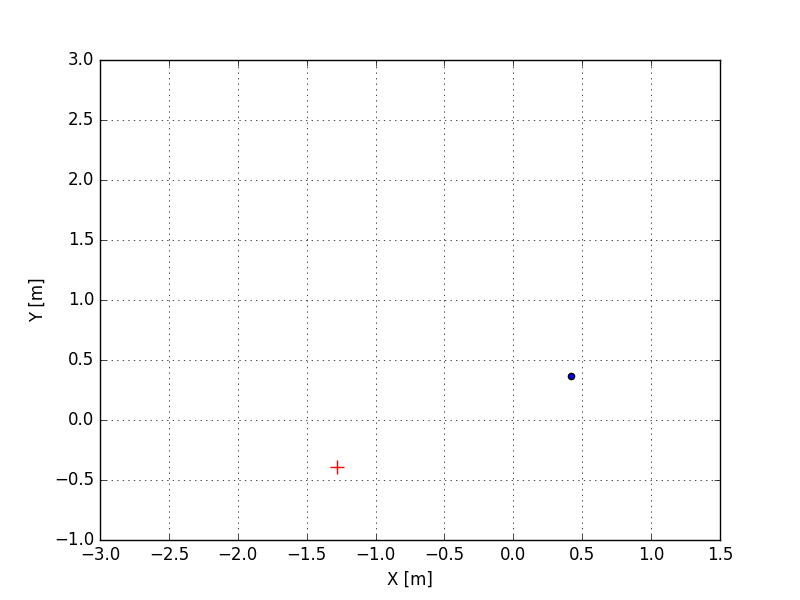
\includegraphics[width=0.7\textwidth]{img/pf-map3-7.png}
\caption{Wyniki lokalizacji za pomocą filtra cząsteczkowego dla ręcznie dobranego modelu - punkt 7}
\end{figure}
\begin{figure}[H]
\centering
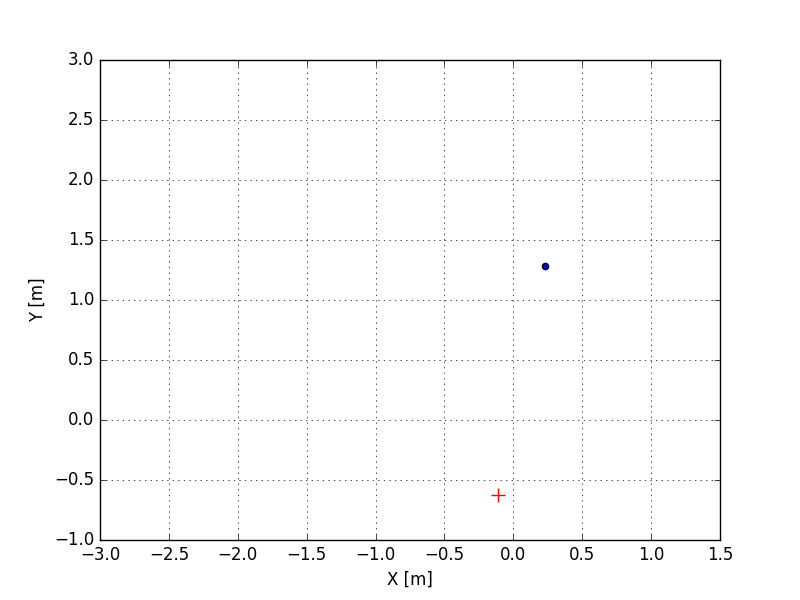
\includegraphics[width=0.7\textwidth]{img/pf-map3-8.png}
\caption{Wyniki lokalizacji za pomocą filtra cząsteczkowego dla ręcznie dobranego modelu - punkt 8}
\end{figure}
\begin{figure}[H]
\centering
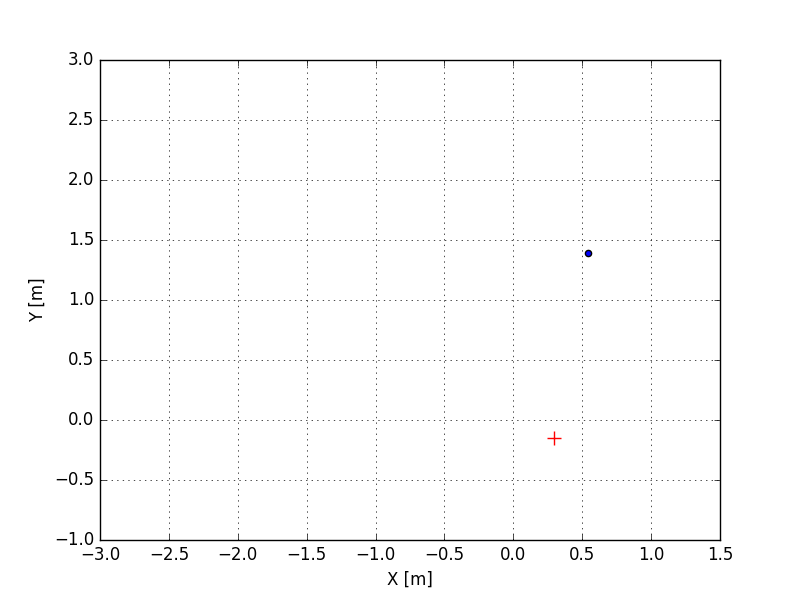
\includegraphics[width=0.7\textwidth]{img/pf-map3-9.png}
\caption{Wyniki lokalizacji za pomocą filtra cząsteczkowego dla ręcznie dobranego modelu - punkt 9}
\end{figure}
\begin{figure}[H]
\centering
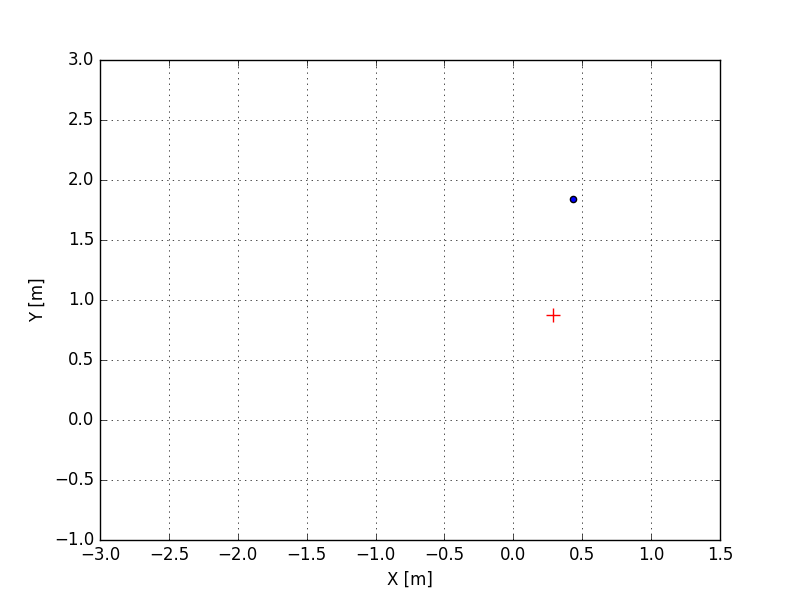
\includegraphics[width=0.7\textwidth]{img/pf-map3-10.png}
\caption{Wyniki lokalizacji za pomocą filtra cząsteczkowego dla ręcznie dobranego modelu - punkt 10}
\end{figure}
\begin{figure}[H]
\centering
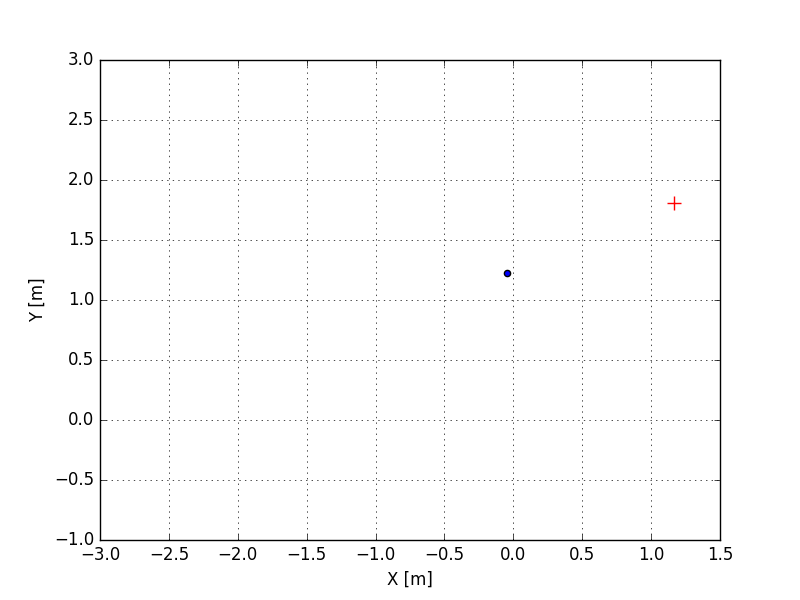
\includegraphics[width=0.7\textwidth]{img/pf-map3-11.png}
\caption{Wyniki lokalizacji za pomocą filtra cząsteczkowego dla ręcznie dobranego modelu - punkt 11}
\label{fig:pf-last}
\end{figure}

\section{Rozwiązanie problemu porwanego robota za pomocą lokalizacji BLE i AMCL}


\clearpage{\pagestyle{empty}\cleardoublepage}

 
\chapter{Wnioski}
\label{ch:wnioski}
\clearpage{\pagestyle{empty}\cleardoublepage}

\phantomsection
\addcontentsline{toc}{chapter}{Bibliografia}
\bibliographystyle{unsrt}	
\bibliography{bibliography}
\clearpage
\phantomsection
\addcontentsline{toc}{chapter}{Wykaz skrótów}
\chapter*{Wykaz skrótów}

\begin{tabular}{l l}
API & Application Programming Interface \\
SDK & Software Development Kit \\


\end{tabular}

